% Modified by Muhammed Yavuzhan CANLI, 25 July 2025

\documentclass[12pt,a4paper]{report}
\usepackage[utf8]{inputenc}
\usepackage[T1]{fontenc}
\usepackage{array}

\usepackage{booktabs}
\usepackage{enumitem}
\usepackage[utf8]{inputenc}
\usepackage[T1]{fontenc}
\usepackage{Bath-CS-Dissertation}
\usepackage{lmodern}         % scalable font fix
\usepackage{float}          

\title{\bf Enhancing Customer Engagement in Physical Casino Environments through Machine Learning-Powered Segmentation and Prediction}
\author{Muhammed Yavuzhan CANLI}
\date{MSc in Computer Science\\
      The University of Bath\\
      Academic Year: 2024--2025\\
      \vspace*{5cm}
      The University of Bath - Ethical Approval: 10351-12382}

\setcounter{secnumdepth}{3}
\setcounter{tocdepth}{3}


%%%%%%%%%%%%%%%%%%%%%%%%%%%%%%%%%%%%%%%%%%%%%%%%%%%%%%%%%%%%%%%%%%%%%%%%%%%%%%%%
%%%%%%%%%%%%%%%%%%%%%%%%%%%%%%%%%%%%%%%%%%%%%%%%%%%%%%%%%%%%%%%%%%%%%%%%%%%%%%%%
%%%%%%%%%%%%%%%%%%%%%%%%%%%%%%%%%%%%%%%%%%%%%%%%%%%%%%%%%%%%%%%%%%%%%%%%%%%%%%%%
\usepackage{amsmath}
\usepackage{amssymb}
\usepackage{url}  

\begin{document}
\sloppy
\tableofcontents


\hypersetup{pageanchor=false}

% Set this to the language you want to use in your code listings (if any)
\lstset{language=Java,breaklines,breakatwhitespace,basicstyle=\small}

\setcounter{page}{0}
\pagenumbering{roman}

\maketitle
\newpage

% Set this to the number of years consultation prohibition, or 0 if no limit
\consultation{0}
\newpage

\declaration{Enhancing Customer Engagement in Physical Casino Environments through Machine Learning-Powered Segmentation and Prediction}{Muhammed Yavuzhan CANLI}

\newpage

\hypersetup{pageanchor=true}

\abstract
The development of artificial intelligence (AI) has created new possibilities for improving decision-making processes in physical casino settings. Traditional casinos encounter structural and technological obstacles in the integration of data sources, including slot logs, ticket-in ticket-out (TITO) systems, and customer relationship management (CRM) databases, unlike online platforms. This dissertation examines the creation of a machine learning framework designed to enhance promotional decision-making within a physical casino environment.

The proposed system employs a hybrid data architecture and applies unsupervised learning through K-Means clustering to classify customers based on behavioural and demographic indicators. A Random Forest classifier is employed to predict engagement levels with targeted promotions, and its performance is evaluated against alternative algorithms (SVM, Decision Tree, and Logistic Regression) to ensure robustness.

The system is organised with a PostgreSQL database backend, Python-based AI modules, and a Docker deployment environment. Data is anonymised, ethically sourced, and processed in accordance with the University of Bath's ethics guidelines (Approval Ref: 10351-12382) \citep{bathEthics}. Real-world behavioural data was made available by Imperial Palace Hotel Casino (Bulgaria), with technical integration and compliance support provided by Mr. Sait Fırat Nemis, IT Manager at Imperial Casino.

This study presents a modular, reproducible, and scalable methodology for customer analytics within the casino sector. The system enables casino IT personnel to make informed, real-time decisions regarding promotion targeting, thus enhancing operational efficiency and customer engagement while maintaining data privacy.



\newpage

\listoffigures
\newpage

\listoftables
\newpage

%%%%%%%%%%%%%%%%%%%%%%%%%%%%%%%%%%%%%%%%%%%%%%%%%%%%%%%%%%%%%%%%%%%%%%%%%%%%%%%%
%%%%%%%%%%%%%%%%%%%%%%%%%%%%%%%%%%%%%%%%%%%%%%%%%%%%%%%%%%%%%%%%%%%%%%%%%%%%%%%%
\chapter*{Acknowledgements}

Add any acknowledgements here.

\newpage
\setcounter{page}{1}
\pagenumbering{arabic}

%%%%%%%%%%%%%%%%%%%%%%%%%%%%%%%%%%%%%%%%%%%%%%%%%%%%%%%%%%%%%%%%%%%%%%%%%%%%%%%%
%%%%%%%%%%%%%%%%%%%%%%%%%%%%%%%%%%%%%%%%%%%%%%%%%%%%%%%%%%%%%%%%%%%%%%%%%%%%%%%%
\chapter{Introduction and Background}

The rise of artificial intelligence (AI) in recent years has profoundly reshaped industries that rely on data-driven decision-making. In particular, the casino industry historically reliant on intuition, human observation, and loyalty-based marketing now stands at a transformative intersection. Unlike online gambling platforms that are inherently digital, physical casinos face more complex challenges when it comes to integrating operational, behavioural, and demographic data sources for intelligent decision-making.

This dissertation addresses the pressing need for a structured, ethical, and technically robust framework that enhances customer engagement in physical casinos. Through the development of an AI-powered decision support system, this research combines customer segmentation with behavioural analytics to support dynamic promotional strategies.



%%%%%%%%%%%%%%%%%%%%%%%%%%%%%%%%%%%%%%%%%%%%%%%%%%%%%%%%%%%%%%%%%%%%%%%%%%%%%
\section{Background}

Customer retention and personal engagement are key success factors in the gambling industry. This is especially true in competitive markets where both physical and online casinos compete for player attention. Online platforms can track user behaviour in detail, but physical casinos often lack integrated systems that connect slot machine logs, ticket-in and ticket-out (TITO) data, CRM systems, and behavioural metrics. As a result, these casinos miss opportunities to personalise promotions and engagement based on customer value and risk levels.

Recent developments in machine learningsuch as clustering and classification algorithmsenable new ways to extract insights from customer data. However, applying these methods in physical casinos is more complex due to operational limitations and strict regulatory requirements. Therefore, the effective and responsible use of AI in this setting requires a combined technical and ethical framework.


%-------------------------------------------------------------------------------
\subsection{The Role of Personalisation in Casino Environments}

Personalisation is fundamental to retention and engagement with customers strategies in diverse sectors, including the casino industry.  In physical casino environments, customising the player experience serves as a competitive advantage and significantly contributes to enhanced dwell time, session value, and overall player satisfaction.

 Traditional casinos frequently depend on visible behavioural indicators and manual customer relationship management strategies to provide a personalised experience.  However, these methods exhibit constraints in both scope and scale.  Digital platforms demonstrate that data-driven personalisation, using customer profiles, interaction history, and predictive modelling, can markedly improve relevance and responsiveness in real time.


 In casinos that are physical, the integration of behavioural data from slot machines, loyalty systems, and ticket-in/ticket-out (TITO) logs enables operators to more effectively segment players and customise offers that align with individual preferences and risk profiles.  A frequent player exhibiting stable betting patterns may receive loyalty bonuses, whereas a high spendingyet unpredictable player could gain more from targeted retention campaigns.

 With the increasing availability of data in casino operations, the potential for applying machine learning to enhance personalisation expands.  This project leverages the identified opportunity to enhance targeted promotional strategies via automated segmentation and response prediction mechanisms.


%-------------------------------------------------------------------------------
\subsection{The Gap Between Online and Physical Casino Analytics}

Online casinos leverage fully integrated digital frameworks that provide real-time monitoring of user activities, preferences, and transaction records.  These platforms frequently utilise sophisticated analytics and recommendation systems driven by machine learning to customise user experiences, enhance promotions, and identify undesirable activity on a large scale.  Each click, spin, and session is carefully recorded, fostering a robust framework for data-informed decision-making.

On the other hand, real casinos often have methods that don't work together.   TITO (Ticket-In Ticket-Out) records, slot machine logs, reward program data, and demographic information are often kept separate or put together by hand.   This lack of cooperation makes it harder for the casino to get a full picture of how players act.   Because of this, marketing strategies used in real stores might be delayed, general, or based on old rules of thumb.

Addressing this gap requires both technological advancement and comprehensive legislation.   Physical casinos face demanding compliance obligations, limited digital presence, and immediate constraints on client interactions.   To achieve comparable analytical capabilities to their online counterparts, these environments must implement anonymised data pipelines, centralised databases, and AI systems that can operate within complex operational frameworks and ethical control.

%-------------------------------------------------------------------------------
\subsection{The Rise of AI-Based Promotional Systems}

%-------------------------------------------------------------------------------

\subsection{Key Concepts}
\subsubsection{Demographics as Predictors of Player Behaviour}

The analysis of age, gender, and nationality plays a crucial role in interpreting gaming behaviours, such as session frequency, risk tolerance, and betting preferences. This study adopts a regionally focused demographic designprimarily players from Bulgaria, Turkey, Greece, and other neighbouring countriesto isolate socio-cultural gaming patterns. These features were algorithmically embedded into anonymised records and integrated into behavioural pipelines, enabling segmentation and promotional targeting models to reflect demographic sensitivities.



\subsubsection{K-Means Clustering}

K-Means clustering is an unsupervised machine learning method employed to segment data into a specified number of groups according to feature similarity.  This method facilitates the identification of unique behavioural profilesnamely Casual, Regular, and High-Value playersby categorising individuals based on their gaming activity patterns, demographic attributes, and engagement metrics.

 The system progressively allocates players to the closest cluster centroid by reducing within-cluster variation.  Upon achieving convergence, each player is linked to a section that represents their comprehensive behavioural and demographic profile.  This enables customised marketing campaigns, as clusters may be analysed and categorised based on corporate goals.

 This study employed K-Means clustering on a dataset enriched with variables including average bet amount, session frequency, loss-chasing behaviour, session volatility, and recent engagement trends.  Furthermore, demographic characteristicssuch as age group, gender, and nationalitywere algorithmically integrated into the feature space to improve cluster differentiation and facilitate socio-cultural segmentation.

 Incorporating demographic characteristics allows the segmentation engine to uncover international gaming behaviours, age-related risk tolerances, and gender-specific promotional reactions.  Preliminary exploratory clustering indicated that younger age groups likely to engage in play more frequently but with lower betting amounts, whereas elderly players may participate less often but with bigger risks.  Additionally, participants from particular national origins demonstrated similar temporal patterns or preferred specific game kinds.

 These insights provide operational value for real-time CRM targeting and establish a basis for more profound study in subsequent rounds of this project, where cross-segment behaviours and promotion response rates will be evaluated.

The K-Means algorithm aims to minimise the intra-cluster variance by assigning each data point to the nearest cluster centroid. This is formalised by the following cost function:

\begin{equation}
\underset{S}{\arg\min} \sum_{i=1}^{k} \sum_{x \in S_i} \| x - \mu_i \|^2
\end{equation}

\begin{itemize}
    \item \( S = \{S_1, S_2, ..., S_k\} \): set of clusters.
    \item \( x \in S_i \): data point \(x\) assigned to cluster \(S_i\).
    \item \( \mu_i \): centroid of cluster \(S_i\).
    \item \(sum_{i=1}^{k}\): The total of these accounts throughout all clusters (e.g., casual, regular, high-value).
    \item arg min: Identify the cluster that minimises this total value. 
\end{itemize}

This function computes the total squared distance between each point and its assigned cluster centre across all \(k\) clusters. The goal is to find a cluster assignment \(S\) that minimises this total distance.

\vspace{0.5em}
\textbf{Example Application:} Suppose we have three customers with average bet values \(\{20, 22, 95\}\). If \(k = 2\) clusters, K-Means may assign \{20, 22\} to one cluster with centroid \(\mu_1 = 21\) and \{95\} to another with centroid \(\mu_2 = 95\), thereby minimising the squared differences:
\[
(20 - 21)^2 + (22 - 21)^2 + (95 - 95)^2 = 1 + 1 + 0 = 2
\]

This objective ensures similar players are grouped, enabling behavioural segmentation and personalised targeting.

In summary, K-Means performs the following:
\textit{``I categorise the players into clusters. However, these clusters must be arranged so that each player is positioned as near as possible to the centre of their group. In this manner, similar players are grouped together.''}


\subsubsection{Random Forest Classifier}

Random Forest is a popular ensemble learning technique that generates multiple decision trees during training and produces the class according to the majority decision across all trees \citet{randomforest}.  In contrast to a single decision tree, which is at risk of overfitting, Random Forest improves generalisation by averaging the predictions of multiple trees trained on diverse bootstrap data sets and groups of features.

Mathematically, given a training dataset \( D = \{(x_1, y_1), \dots, (x_n, y_n)\} \), Random Forest constructs \( T \) decision trees \( \{h_1(x), h_2(x), \dots, h_T(x)\} \), where each \( h_t \) is trained on a random subset of \( D \). For classification, the ensemble output \( H(x) \) is defined as:

\[
H(x) = \text{mode}\left( h_1(x), h_2(x), \dots, h_T(x) \right)
\]

This election method fixes predictions and facilitates probabilistic outputs. For instance:  
\textit{``Player A has a 74\% probability of accepting the promotion based on their loss pattern, session duration, and customer segment.''}

This research employs Random Forest to predict the possibility of promotional approval based on behavioural features, including:

\begin{itemize}
    \item Average session loss
    \item Duration and frequency of play
    \item Segment membership (e.g., Casual, High-Value, Regular)
    \item Engagement trend (e.g., bet increase/decrease)
    \item Demographic inputs (age group, gender, nationality)
\end{itemize}

\paragraph{Illustrative Example:}To illustrate how Random Forest works in the context of casino promotions, consider the following scenario:

\begin{quote}
    A casino is evaluating the potential implementation of a promotion for Player-A.  Several decision trees are developed applying historical data, with each tree employing different player subsets and features including age, gender, session duration, and loss amount.
    
    \begin{itemize}
        \item Tree-1 predicts: \texttt{Yes}
        \item Tree-2 predicts: \texttt{Yes}
        \item Tree-3 predicts: \texttt{No}
        \item Tree-4 predicts: \texttt{Yes}
        \item Tree-5 predicts: \texttt{Yes}
    \end{itemize}
    
    Out of 5 trees, 4 suggest offering a promotion. Therefore, the final output of the Random Forest is: \textbf{Yes, with 80\% confidence}.
\end{quote}

This simple majority voting method allows Random Forest to generate consistent and accurate projections, even when individual decision trees may be poor or overfitted.  The probabilistic output (e.g., 80\% likelihood) allows CRM systems to rank or filter participants according to probability, therefore prioritising marketing initiatives.

 A major advantage of Random Forest is its inherent capability of evaluating feature importance, measuring the contribution of each input variable to overall prediction effectiveness.   This enables transparency and clarity, which are particularly crucial in regulated environments such as casinos, where understanding the impact of demographic elements is essential for responsible and ethical promotional decision-making.


\subsubsection{ML vs Rule-Based Systems}

Traditional rule-based systems in casinos function through established "if-then" logic, where particular thresholds activate promotional or operational reactionssuch as granting a bonus following a loss of 1000 or delivering notifications dependent on the time of day.  These systems show transparency and allow for auditing; nevertheless, they lack adaptation to dynamic behavioural patterns and are not capable of detecting underlying behavioural trends.

 On the contrary, machine learning (ML) methodologiessuch as K-Means clustering and Random Forest classificationfacilitate pattern recognition through the analysis of historical data.  These models clarify non-linear and complicated interactions, such as recognising that players of a particular nationality, within a defined age brackets, and exhibiting rapid recovery from losses may exhibit enhanced responsiveness to specific rewards.

 Machine learning systems provide probabilistic predictions rather than binary rule outputs, assigning probability scores to client behaviours.  This facilitates complex decision-making, for instance, "Player A has a 74\% probability of accepting a cashback promotion," so benefiting in prioritisation and risk-adjusted intervention strategies.  However, machine learning models require a resilient data infrastructure, validation methodologies, and ethical protections, especially in regulated sectors such as gaming.

 This study employs a rule-based methodology as a comparative benchmark, while the machine learning pipeline is engineered to provide scalable, real-time, and ethically acceptable promotion methods.  The two paradigms are utilised simultaneously to combine interpretability with predictive efficiency.

\vspace{0.2cm}
\textbf{Example Paradigms}:
\begin{itemize}
    \item \textbf{Rule-Based:} ``If a customers net loss exceeds 1000, then offer a standard promotion.''
    \item \textbf{ML-Based:} ``There is a 74\% probability that this customer will respond positively to a cashback offer, based on session length, recent losses, and demographic profile.''
\end{itemize}

%-------------------------------------------------------------------------------

\section{Problem Statement}

Problem Statement

 Despite major investments in digital infrastructure, many physical casinos continue in utilising static and intuition-based promotional strategies.  These approaches are generally predefined and lack the adaptability necessary to detect real-time variations in player activity.  Consequently, chances to improve player engagement, retention, and lifetime value are often ignored.

In an increasingly competitive environment where both digital and physical entities compete for attention, understanding player profiles has become essential.  Critical behavioural markers, such as session duration, alterations in bet size, recent loss patterns, and frequency of play, offer substantial insights.  Without accurate measurement and assessment of these characteristics, traditional casinos struggle to tailor promotional offers or recognise high-value and at-risk customers.

The lack of dynamic segmentation, real-time behavioural scoring, and predictive modelling decreases marketing efficiency and enhances the possibility of violating responsible gambling regulations. Lack of ability to identify loss-chasing behaviours or player exhaustion may result in reputational harm or regulatory penalties. Furthermore, most promotional datasets have a significant class imbalance, meaning that most players do not interact with campaigns. This makes it even more difficult to train models and conduct successful targeting.


 This study presents a modular and scalable AI-driven architecture that integrates multi-source data, including slot logs, TITO, and CRM records, within a compliant PostgreSQL framework to overcome these limitations.  The method uses unsupervised clustering and supervised classification to produce promotional decisions tailored to specific segments.  This approach is intended to function within the operational limitations of physical casinos while supporting ethical, real-time decision-making via comprehensible machine learning techniques.


\section{Overview and Scope}

This dissertation constructs, executes, and assesses a comprehensive AI-driven pipeline aimed at improving promotional decision-making in physical casino settings. The suggested approach integrates behavioural data with synthetic demographic characteristics to facilitate ethical and customised client involvement. The architecture is modular, scalable, and engineered for technical feasibility in actual casino operations.

The solution consists of two core components:

\begin{itemize}
    \item \textbf{Hybrid Data Integration Layer:} Behavioural dataincluding slot machine logs and TITO transactionsare consolidated with synthetically generated demographic attributes (age, gender, nationality) into a PostgreSQL database. All records are anonymised to ensure full compliance with GDPR and BATH regulations. The database schema was designed and implemented by the author, supporting structured, queryable datasets for downstream machine learning processes.
    
    \item \textbf{AI-Based Decision Engine:} A two-stage machine learning strategy is adopted. First, unsupervised K-Means clustering segments players into behavioural groups (e.g., Casual, Regular, High-Value). Then, a Random Forest classifier predicts individual promotional responsiveness, using behavioural features such as average loss, session duration, and volatility indicators. Additional mechanismssuch as loss-chasing detection and temporal engagement labellingare integrated to support responsible gambling.
\end{itemize}

The pipeline is fully automated using Python modules and is deployable through a Docker-based environment. Although the system does not directly interface with a live CRM, it provides segment labels and promotion decision flags in export-ready formats compatible with casino marketing operations.

Overall, the system is designed to support ethical, transparent, and data-driven promotional strategies that respect both player privacy and operational practicality.

\begin{figure}[H]
\centering
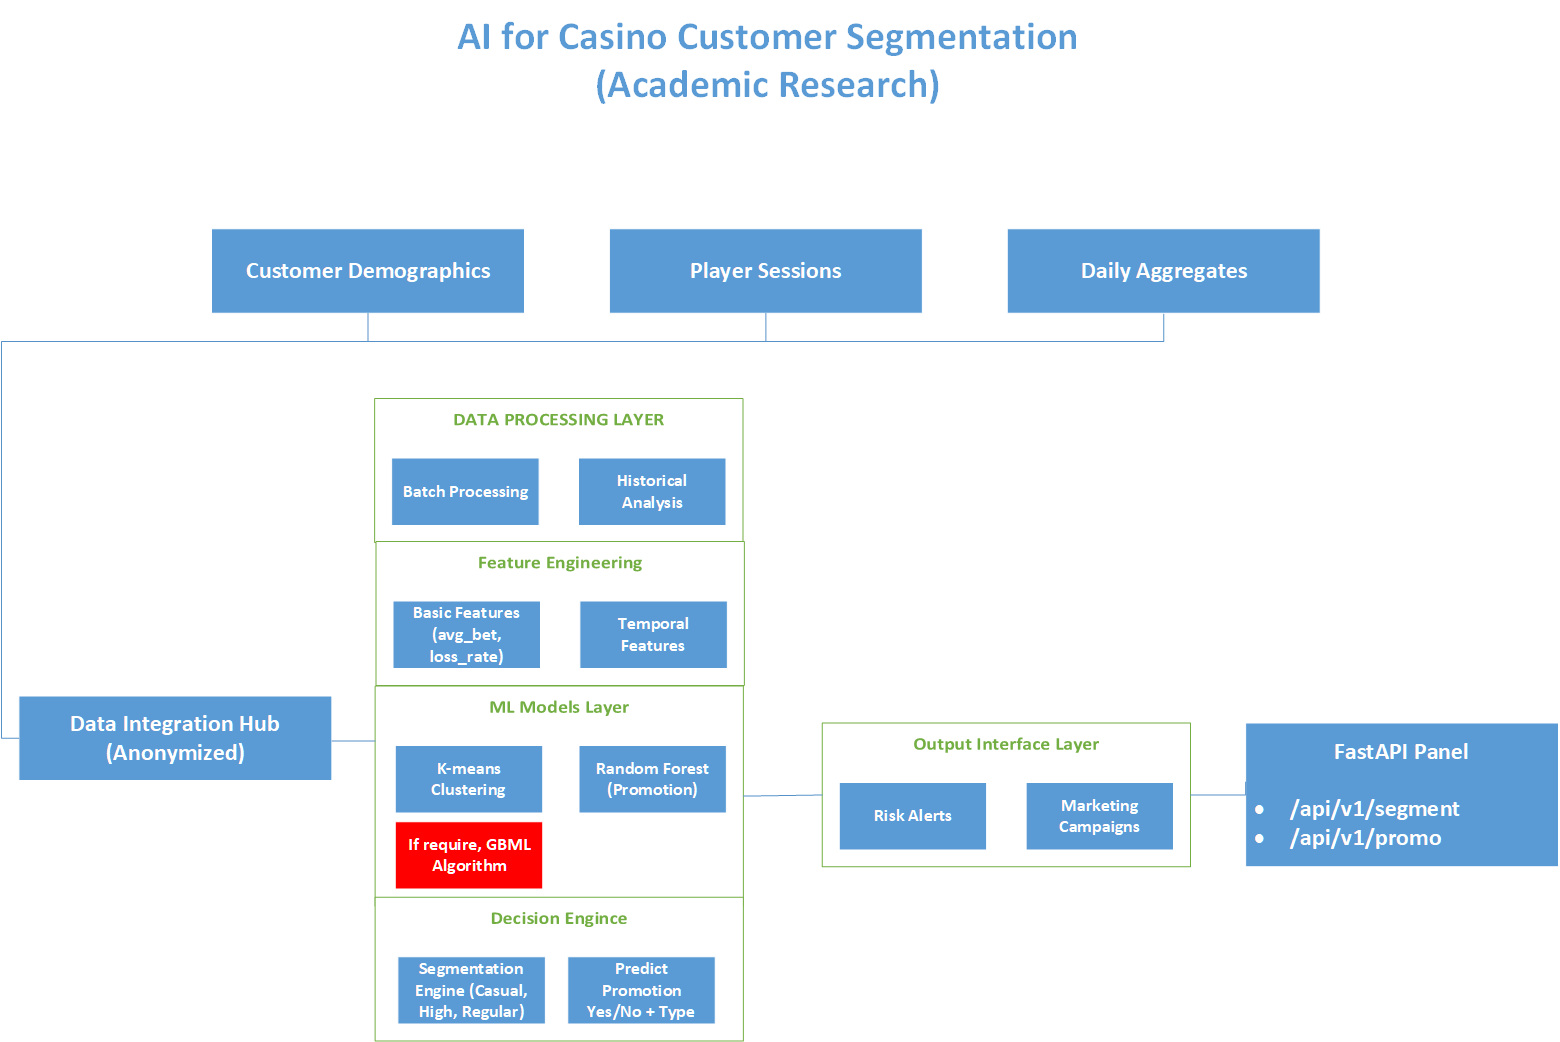
\includegraphics[width=0.9\textwidth]{figures/project_overview_diagram.png}
\caption{Project Overview: Modular Architecture Integrating Anonymised Data, Feature Engineering, and ML-Driven Promotional Decision-Making}
\label{fig:overview and scope}
\end{figure}

Illustrates the overall AI pipeline and data integration strategy. It highlights how anonymised inputs from slot logs, demographic synthesis, and behavioural records flow through the processing layer and machine learning modules to support intelligent promotional decisions and segment-aware CRM interventions.

\subsection{System Architecture and Project Pipeline Overview}
The suggested system's design is organised into a modular pipeline that integrates data ingestion, preprocessing, unsupervised clustering, supervised classification, and promotion flagging. Each module was created utilising Python and follows to a reproducible, testable approach incorporated within a Dockerized environment.

\begin{itemize}
    \item \textbf{Data Ingestion Layer:} Involved the cleaning, validation, and importation of raw behavioural logs from slot machines and TITO transactions into a PostgreSQL database. Synthetic demographic variablesage group, gender, and nationalitywere algorithmically generated using the synthetic data toolkit to emulate CRM-like completeness while maintaining GDPR and University compliance \citep{faker2025}.

    \item \textbf{Feature Engineering:} Custom Python modules were utilised to extract behavioural metrics, including average bet, session duration volatility, loss-chasing indicators, and recent engagement trends. The features were organised within a specific \texttt{customer\_features} table, serving as the foundation for both clustering and classification processes.

    \item \textbf{Unsupervised Segmentation (K-Means):} Customers were grouped into segments (e.g., Casual, Regular, High-Value) using K-Means clustering. Segment assignments were stored in a separate table and served as contextual inputs for subsequent analysis.

    \item \textbf{Supervised Classification (Random Forest):} Applying the engineering features and segment labels, a Random Forest model forecasted clients' probability to engage with a proposition.  The outputs consist of a probability of promotion response and a recommended action level.

    \item \textbf{Export and Deployment:} Final outputscomprising segment labels and promotion decisionswere made export-ready for CRM teams in CSV format. The pipeline supports both batch execution and future real-time API-based inference, depending on deployment needs.

\end{itemize}

\begin{figure}[H]
\centering
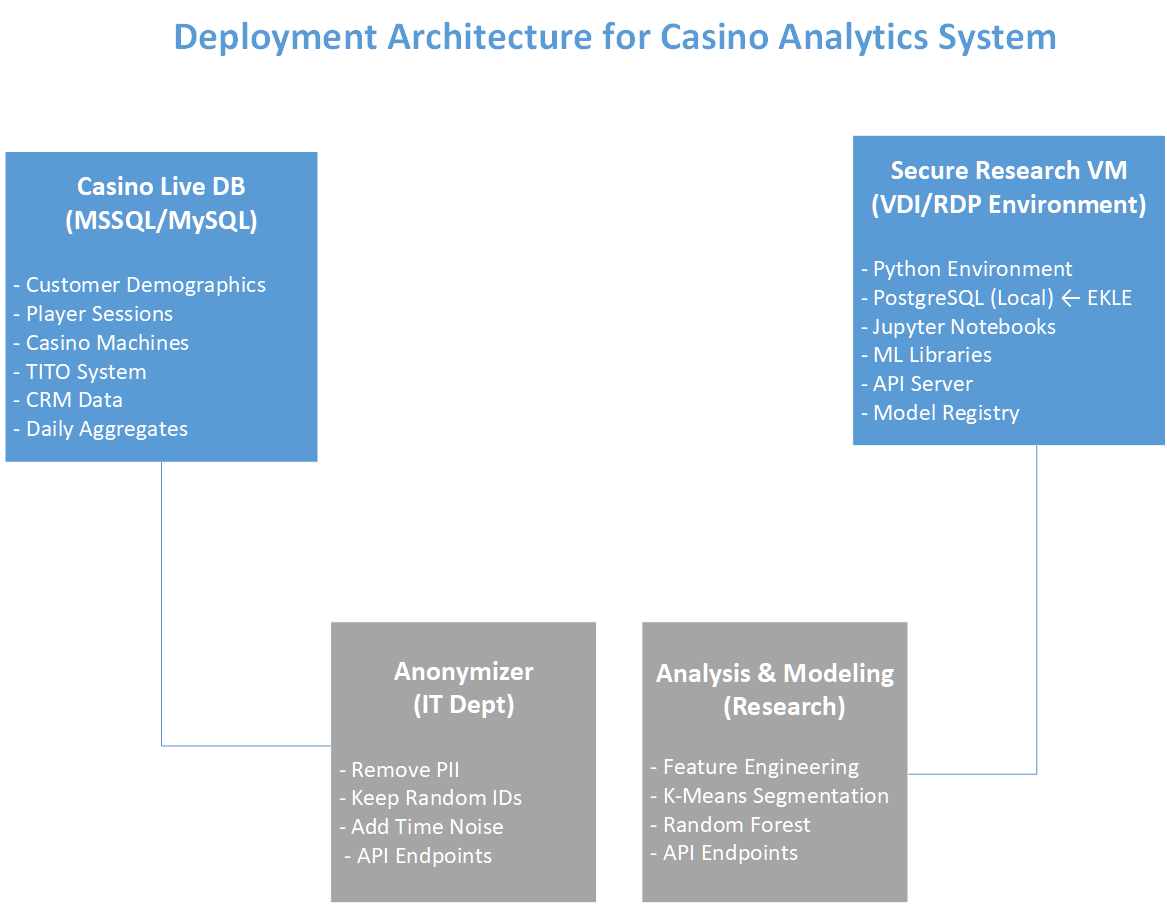
\includegraphics[width=0.85\textwidth]{figures/casino_analytics_system.png}
%\caption{Deployment Infrastructure for Casino Analytics System: DB, VM, and Security Layers}
\label{fig:deployment-architecture}
\end{figure}


Figure~\ref{fig:deployment-architecture} Illustrates the systems deployment and anonymisation flow between live databases and the research environment.


\subsection{Data Context and Research Setting}

This research is carried out in the context of a physical casino in Eastern Europe, utilising anonymised player data gathered from slot machine activity, ticket-in ticket-out (TITO) logs, and historical customer relationship management (CRM) interactions.  The main data sources consist of two live relational databasesMSSQL and MySQLintegrated via secure anonymisation protocols and subsequently transferred to a PostgreSQL research environment. 

 This study utilises 12 months of behavioural logs from January to December 2022, encompassing more than 30,000 unique player records.  In the absence of comprehensive demographic data, synthetic demographic attributes, including age group, gender, and nationality, have been produced algorithmically as a synthetic data using Python's library. This approach ensures GDPR and BATH compliance while facilitating socio-demographic segmentation \citep{gdpr2016}.

 The data was accessed through remote desktop protocol (RDP) with supervision from the casinos IT department, ensuring compliance with ethical guidelines approved under reference 10351-12382 by the University of Bath.  Personally identifiable information (PII) was excluded at the source, and all customer identifiers were either hashed or pseudonymized.

 The controlled environment guided the simulation of real-world marketing scenarios while following to data privacy regulations.  The research setting demonstrates a pragmatic design that emulates operational casino systems, providing a flexible and modular framework for academic experimentation.


\subsection{System Objective and Target Use Case}


\subsection{CRM Compatibility and Real-Time Utility}


%-------------------------------------------------------------------------------
\section{Contributions}

The goal of this study was to create AI-based solutions for high-frequency transactional settings, where customer behaviour can be tracked and dealt with in real time.  The gambling domain has a special mix of high transaction volume, a wide range of users, and marketing responsiveness.  Unlike more established AI fields like healthcare or e-commerce, retail,gaming, especially physicalcasinos, hasn't been studied much in university AI applications.  This project aims to fill that gap by mixing real data, ethical design principles, and an AI pipeline that can be used in any way.

As a researcher, "I deliberately selected a domain with high transaction volume but relatively low academic saturation in AI implementation, enabling more originality and freedom for system design."

The dissertation presents the following key contributions:

\begin{itemize}
    \item A hybrid data architecture that integrates slot machine logs and TITO records, producing CRM-compatible outputs, within a PostgreSQL database.
    \item A Python-based modular AI pipeline engineered for scalability and delivered via Docker, featuring custom feature engineering that encompasses behavioural volatility and loss-chasing detection.
    \item A segment-aware Random Forest model for promotional decision-making, underpinned by comparison analysis across client segments.
    \item A comparative model analysis and promotional decision-support logic.
\end{itemize}

\subsection*{1.4.1 Use of Generative AI Tools (Type B Declaration)}

Throughout the composition of this dissertation, the use of generative AI tools was restricted in accordance with the University of Bath's directives on Type B assessments. ChatGPT-4 (OpenAI, \url{https://chat.openai.com/}) was utilised to aid in the preliminary creation of some non-essential code segments and to validate Python syntax throughout the implementation stage.

The AI aid was restricted to the subsequent activities:
\begin{itemize}
    \item Validating and troubleshooting common Python constructs (e.g., pandas joins, stratified K-Fold validation)
    \item Analysing usage patterns of sklearn, such as parameters of RandomForestClassifier  \citep{scikit-learn}
    \item Proposing a framework for modular pipeline components, such as model evaluation functions
    \item Establishing preliminary formatting for visualisation code (matplotlib/seaborn)
\end{itemize}

All AI-generated content was examined, modified, and incorporated by the author, and no directly replicated code or text was utilised in the final dissertation. The conceptual design, technical rationale, implementation choices, and integration with the PostgreSQL/Docker pipeline were completely created and owned by the student. The utilisation of AI was not crucial for the project's completion and functioned only as an additional coding assistant.

%-------------------------------------------------------------------------------

%%%%%%%%%%%%%%%%%%%%%%%%%%%%%%%%%%%%%%%%%%%%%%%%%%%%%%%%%%%%%%%%%%%%%%%%%%%%%%%%
%%%%%%%%%%%%%%%%%%%%%%%%%%%%%%%%%%%%%%%%%%%%%%%%%%%%%%%%%%%%%%%%%%%%%%%%%%%%%%%%
\chapter{Literature and Technology Survey}

The convergence of artificial intelligence (AI), demographic analytics, and customer engagement represents a critical domain of innovation in the casino industry.  Although considerable research has investigated the implementation of machine learning in online gaming platforms, the use of AI-driven systems in physical casino settings is still restricted.  This chapter provides a critical examination of recent studies related to fundamental concepts, technologies, and models linked to AI-driven segmentation, prediction, and operational optimisation in casinos.   This review analyses clustering techniques, including K-Means, and evaluates supervised models such as Random Forest, while comparing various algorithms. It also explores the influence of demographics on player behaviour and discusses frameworks for responsible gambling. Additionally, technological frameworks like TITO systems, which offer readily available data for CRM integration, and real-time data pipelines are examined in the context of recent advancements.

\section{Artificial Intelligence in Casino Environments}
Recent advancements in artificial intelligence have enabled new forms of player engagement and dynamic personalisation in casino operations \citep{Auer2023, Omike2022a}. Studies show that predictive model Random Forest can increase player retention and optimise marketing strategies \citep{Ladouceur2016}.


\section{Demographic Segmentation and Behavioural Profiling}

Understanding the influence of demographic attributes on gambling activity is crucial for customer segmentation and targeted marketing strategies in physical casino environments.  Important demographic characteristics, including as age, gender, nationality, and socioeconomic status, have been shown to correlate with gaming preferences, betting habits, and overall engagement duration \citep{Hing2014}. For instance, younger players are typically linked to frequent, low-value gaming sessions, whereas older groups generally engage in longer play periods and make greater average wagers \citep{Desiata2024b}.

Segmenting casino customers based on demographic factors provides operational advantages such as personalised promotions, game-floor layout optimisation, and differentiated loyalty schemes. Studies have highlighted that tailored communication based on language or cultural preferences can increase return visits and ticket-in amounts \citep{Abarbanel2022}. Additionally, nationality-specific clustering has discovered behavioural differences; for example, visitors from the Balkan region demonstrate distinct slot preferences in contrast to those from Western Europe.

However, demographic segmentation in isolation may not be sufficient to predict customer lifetime value or risk profiles. Researchers advocate for combining demographic profiles with behavioural and transactional data to create multi-dimensional customer personas \citep{Ladouceur2016}. In line with this, our study integrates demographic attributes into behavioural clustering and prediction tasks, using them as input features for model training.

Data collected from physical casinos, particularly in multi-national tourist zones, presents unique opportunities for demographic profiling. Our dataset reflects such diversity, including anonymised player information across nationalities such as Bulgaria, Germany, Greece, Turkey, and the Netherlands. These insights are crucial for developing AI-powered recommendation systems that align with players' cultural expectations and risk tolerance.


\section{Clustering and Classification Algorithms}

Machine learning has enabled a wide range of data-driven strategies in casino analytics, particularly for customer segmentation and behavioural prediction. This study adopts a hybrid approach that leverages both unsupervised and supervised learning algorithms, tailored to the characteristics of anonymised player data collected from physical casino environments.

\subsection{K-Means Clustering}

K-Means is a widely used unsupervised algorithm for partitioning customers into behavioural segments.  The process involves minimising intra-cluster variance and allocating players to the nearest centroid within the feature space \citep{MacQueen1967}. K-Means clustering has been used in casino contexts to categorise players according to session duration, loss volatility, zone diversity, and average bet size.\citep{Desiata2024a}. The simplicity and interpretability of the algorithm make it especially suitable for initial segmentation in real-time applications.

This project utilised K-Means to categorise customers into three primary groups: Casual, Regular, and High Roller players.  The identified segments formed the foundation for informed promotional decision-making in later classification tasks.  The clustering analysis was carried out over several six-month intervals to assess customer migration patterns and temporal consistency.

\subsection{Random Forest Classifier}

Random Forest is a supervised ensemble learning technique that takes decision trees, recognised for its strength and ability to generalise effectively \citep{Breiman2001}. It generates several decision trees and consolidates their outcomes to produce final predictions, hence mitigating overfitting.  The model has demonstrated efficiency in managing behavioural datasets characterised by heterogeneous feature types and partly missing values \citep{Auer2023}.

The present study utilised Random Forest to forecast a player's probability to respond positively to promotional offers.  Features obtained from demographic and behavioural sourcesincluding loss-chasing scores, recent activity levels, and section labelswere utilised in the training process.  Cross-validation results indicated that Random Forest surpassed baseline classifiers, including Logistic Regression and Decision Trees, over various intervals.

\subsection{Gradient Boosting as an Alternative}

While Gradient Boosting Machine Learning (GBML) was not applied in this work, it continues to be an impressive option to Random Forest.  GBML develops cumulative models progressively, enhancing weak learners to reduce prediction error \citep{Omike2022b}.Research comparing GBML and RF in gaming contexts suggests that GBML may provide higher precision in certain situations, although with heightened complexity and reduced clarity.

Due of the real-time objectives and interpretability requirements of physical casino systems, Random Forest was deemed the best suitable classifier.  Future endeavours may involve the application of GBML models to assess their effectiveness in high-precision targeting contexts.

\section{Responsible Gambling and Ethical AI}

The importance of ethical questions surrounding responsible gambling has grown in recent years, especially with the increasing integration of AI-driven systems into casino operations.  Regulations like the General Data Protection Regulation (GDPR) place severe constraints on the collection, processing, and use of personal and behavioural data \citep{gdpr2016}. In physical casinos, these concerns get worse by the real-time nature of player tracking and the risk of accidentally targeting vulnerable individuals.

The goal of engaging in responsible gambling is to reduce negative outcomes by recognising and addressing problematic gambling behaviours.  Several studies stress the significance of integrating behavioural risk indicators into AI decision-making pipelines. These signs can include long session durations, unexpected bet changes, or a tendency to chase losses \citep{Ladouceur2016, Priyadarshini2022}. These indications not only safeguard vulnerable players but also conform to the ethical obligations of operators.

This study employs a privacy and preserving methodology in accordance with GDPR and ethical research norms. All client data utilised in model training was entirely anonymised by the application of synthetic identities and manufactured demographic profiles developed using the Faker library \citep{faker2025}. Furthermore, segmentation and prediction results were evaluated against false-positive risks to prevent marketing offers to players displaying potential indicators of problem gambling.

Honesty and understanding are also aspects of ethical design.  The promotional decision system explored using rule-based overrides to guarantee human-in-the-loop evaluation in extreme instances.  According to Abarbanel and Phung (2022), designing gaming technology in a way that is both transparent and culturally sensitive helps to build trust among users and encourages long-term participation.

\section{Casino Technologies: TITO, CRM and Data Pipelines}

Transactional systems and customer records are used together in modern casinos to make sure that each player has a personalised experience and that staff can keep an eye on what players are doing.  Ticket-In Ticket-Out (TITO) systems were first made to replace coin-based payouts. Now they are a great way to collect information about how people behave.  Each ticket stores timestamps, machine interactions, and financial values. These can be put together to get session-level insights and trends of loss-chasing \citep{Nemis2024}.

Platforms for customer relationship management, or CRM, are another essential element, particularly when it comes to retaining valuable players.  Promotion history, contact preferences, and demographic information are frequently stored in these platforms.  However, in physical casinos, where several systems may function independently, integrating CRM data with real-time behavioural signals continues to be a challenge \citep{Wayne2024}.

The vital connection between these different sources and AI-powered decision engines is provided by data pipelines.  Scalable prediction systems must be able to ingest, process, and transform real-time game logs in high-frequency settings like casinos.  In order to facilitate prompt feature engineering and promotional decisions, technologies like PostgreSQL in conjunction with RESTful APIs or Kafka-style stream processors are being utilised more and more.  Although the potential of such structures has been shown in earlier research on online gambling, their use in traditional contexts is still in the early stages \citep{Omike2022a}.

The hybrid data architecture used in this study combines slot machine telemetry, CRM profiles, and TITO logs into a single AI pipeline.  While following to ethical and privacy norms, this infrastructure facilitates real-time segmentation and predictive modelling.

\section{Research Gap and Summary}

While significant progress has been made in applying AI to online gambling platforms, there is a noticeable gap in literature addressing the deployment of machine learning in physical casino environments. Most existing studies focus on digital contexts with controlled environments, where user data is consistently structured and readily available \citep{Auer2023, Omike2022a}. In contrast, real-world casino data is often fragmented, partially anonymised, and lacks standardisation, making model development and deployment considerably more challenging.

Furthermore, the integration of demographic data with behavioural indicators remains underexplored. Although some research has acknowledged the influence of age, gender, and nationality on gambling behaviour \citep{Hing2014, Desiata2024a}, few studies have systematically incorporated these features into real-time AI pipelines for segmentation and promotion. Similarly, while clustering algorithms such as K-Means and classifiers like Random Forest have been evaluated in isolation, comparative and integrated applications in operational casino environments are limited \citep{MacQueen1967, Breiman2001}.

The lack of responsible gambling mechanisms within AI-driven casino decision systems also presents an ethical void. Existing literature has called for more interpretable and fair systems \citep{Ladouceur2016, Abarbanel2022}, yet practical frameworks for combining ethical oversight with predictive analytics remain rareparticularly in non-digital venues.

This dissertation addresses these gaps by developing an end-to-end AI-powered customer engagement framework tailored for physical casinos. The system integrates demographic segmentation, behavioural feature engineering, and predictive modelling within a privacy-preserving, real-time data architecture. It contributes to the field by bridging theoretical AI models with real-world deployment constraints and ethical considerations in a regulated environment.


%%%%%%%%%%%%%%%%%%%%%%%%%%%%%%%%%%%%%%%%%%%%%%%%%%%%%%%%%%%%%%%%%%%%%%%%%%%%%%%%
%%%%%%%%%%%%%%%%%%%%%%%%%%%%%%%%%%%%%%%%%%%%%%%%%%%%%%%%%%%%%%%%%%%%%%%%%%%%%%%%
\section{Overview of System Goals and Constraints}

The goal of this project is to create and use an AI-powered decision support system that makes customers more interested in going to real-life casinos by dividing them into groups in real time and predicting who they will be interested in what promotions they will see.  By using flexible machine learning models, the main goal is to close the gap between the rich behavioural data that is collected on-site and marketing insights that can be put into action.

The system is engineered to process client data from many sources, including Ticket-In Ticket-Out (TITO) logs, client Relationship Management (CRM) profiles, and slot machine telemetry.  The diverse inputs are consolidated via a PostgreSQL-supported data pipeline and are utilised in both clustering (K-Means) and classification (Random Forest) models.

Key objectives of the system include:

\begin{itemize}
  \item Segmenting players into behavioural groups to enable targeted marketing strategies.
  \item Predicting promotional responsiveness to minimise marketing waste and improve ROI.
  \item Ensuring compliant data handling through anonymisation and consent-aware logic.
  \item Supporting both batch and real-time workflows for flexibility in deployment.
  \item Providing explainable results that can be reviewed and adjusted by CRM managers.
\end{itemize}

However, several operational and ethical constraints must be acknowledged. Real-world casino environments are constrained by limited data access, system integration issues, and the need for real-time responsiveness. Moreover, ethical requirements such as fairness, transparency, and responsible gambling must be integrated into every decision-making layer. These constraints directly influence the architecture, feature selection, and model design choices adopted throughout this dissertation.

\section{Functional and Non-Functional Requirements}

The system requirements for the proposed AI-powered casino engagement framework are categorised into functional and non-functional requirements. These requirements were derived through iterative development, literature-informed design principles, and real-world casino data constraints.

\section{Functional and Non-Functional Requirements}

A two-phase implementation strategy is employed to define the requirements of the proposed AI-based casino engagement framework: an exploratory phase (Casino-1) that employs synthetic datasets, and a production-aligned phase (Casino-2) that employs anonymised bulk data from real operational sources.  Non-functional requirements define how the system should perform under a variety of constraints, such as ethical, legal, and performance aspects, while functional requirements specify what the system must do.

\subsection{Functional Requirements}

\begin{enumerate}[label=FR\arabic*:]
  \item \textbf{Customer Anonymisation:} The system shall anonymise all customer identifiers using GDPR-compliant formats (e.g., \texttt{CUST\_XXXXXX}).\hfill \textit{(High)}
  
  \item \textbf{Synthetic Demographics:} The system shall generate synthetic demographic attributes (age range, gender, nationality) when they are unavailable, thereby guaranteeing compliant pseudonymization \hfill \textit{(High)}
  
  \item \textbf{Secure Storage:} Demographic data shall be stored in the PostgreSQL schema \texttt{casino\_data.customer\_demographics}.\hfill \textit{(High)}
  
  \item \textbf{Feature Engineering:} The system shall extract behavioural features (e.g., \texttt{avg\_bet}, \texttt{loss\_rate}, \texttt{session\_duration}, \texttt{zone\_diversity}) from gameplay logs.\hfill \textit{(High)}
  
  \item \textbf{Customer Segmentation:} All active customers shall be segmented into \textit{Casual}, \textit{Regular}, and \textit{High Roller} groups using the K-Means algorithm.\hfill \textit{(High)}
  
  \item \textbf{Promotion Prediction:} A Random Forest classifier shall predict whether a promotion should be sent to a customer based on behavioural and demographic features.\hfill \textit{(High)}
  
  \item \textbf{Versioned Output:} All model outputs shall be saved with metadata under \texttt{casino\_data.customer\_features} for traceability.\hfill \textit{(Medium)}
  
  \item \textbf{REST API:} A RESTful endpoint shall return a customer's segment and promotion status upon querying by customer ID.\hfill \textit{(Medium)}
  
  \item \textbf{Multi-Source Ingestion:} The system shall support data ingestion from batch (.csv) and live session logs (MSSQL, MySQL).\hfill \textit{(Medium)}
  
  \item \textbf{Decision Logging:} Each AI decision shall be logged with timestamp, customer ID, and associated prediction probability for auditability and A/B testing.\hfill \textit{(Medium)}
\end{enumerate}

\subsection{Non-Functional Requirements}

\begin{enumerate}[label=NFR\arabic*:]
  \item \textbf{GDPR Compliance:} All personal data must be anonymised and pseudonymised in accordance with Article 26 of GDPR.\hfill \textit{(High)}
  
  \item \textbf{Reproducibility:} All model training pipelines and outputs shall be version-controlled and reproducible under fixed seeds and documented configurations.\hfill \textit{(High)}
  
  \item \textbf{Batch Performance:} The system shall complete segmentation for 50,000 customers within 5 minutes in offline mode.\hfill \textit{(Medium)}
  
  \item \textbf{Real-Time Response:} Prediction API endpoints shall respond within 300 milliseconds under normal server conditions.\hfill \textit{(Medium)}
  
  \item \textbf{Secure Connections:} All external database connections (e.g., MSSQL) shall use encrypted channels (e.g., over VPN/RDP).\hfill \textit{(High)}
  
  \item \textbf{Explainability:} Each prediction shall be stored alongside feature importances and timestamp for audit and human-in-the-loop review.\hfill \textit{(High)}
  
  \item \textbf{Modularity:} The system shall be designed modularly to allow the integration of new features or model types without architectural rewrites.\hfill \textit{(Medium)}
  
  \item \textbf{Bias Prevention:} Synthetic data generation shall maintain demographic balance to prevent model bias across age, gender, and nationality groups.\hfill \textit{(High)}
  
  \item \textbf{Academic Compliance:} All code, data access, and documentation shall comply with University of Baths ethical research standards and academic integrity guidelines.\hfill \textit{(High)}
  
  \item \textbf{Data Confidentiality:} Sensitive data files shall be excluded from public repositories and stored securely in protected storage environments.\hfill \textit{(High)}
\end{enumerate}

\section{Data Requirements and Ethics Constraints}

The system depends on consumer and transactional data from real casino settings, derived from three main sources: Ticket-In Ticket-Out (TITO) logs, slot machine telemetry, and consumer Relationship Management (CRM) profiles.  The data types vary in structure and granularity, requiring schema-aware input and preprocessing mechanisms.

\subsection*{Data Sources and Structure}

To test its early algorithms, the system's prototype (Casino-1) employed XML, CSV, and JSON files containing synthetic data.  Alternatively, a PostgreSQL-based pipeline was utilised in the final implementation (Casino-2) to load pre-anonymized transactional logs produced from MSSQL and MySQL systems.  The most important ones were:

\begin{itemize}
  \item \textbf{Slot Logs:} Session-level gameplay data including \texttt{bet\_amount}, \texttt{win\_amount}, \texttt{RTP}, \texttt{symbol\_patterns}, \texttt{session\_duration}.
  \item \textbf{TITO Logs:} Ticket-based cash flow data covering \texttt{ticket\_in}, \texttt{ticket\_out}, and jackpot contributions.
  \item \textbf{CRM Data:} Demographic attributes such as age, gender, nationality, VIP status, registration month, and communication preferences.
\end{itemize}

With timestamps included in every log entry, trend and volatility calculations are made possible, which greatly helps in temporal analysis and customer lifecycle modelling.

\subsection*{Anonymisation and GDPR Compliance}

In compliance with Article 26 of the General Data Protection Regulation (GDPR), the system applies a pseudonymisation protocol where customer identifiers are replaced with randomised, irreversible tokens in the format \texttt{CUST\_XXXXXX}. This ensures that individual identities cannot be inferred, even when multiple data sources are cross-linked.

Additionally:

\begin{itemize}
  \item Raw age values are converted into categorical ranges (e.g., 1824, 2534) to prevent individual reidentification.
  \item No names, email addresses, phone numbers, or biometric data are used or processed at any stage.
  \item All CRM demographic data were either anonymised or synthetically generated using the \texttt{Faker} Python library \citep{faker2025}.
\end{itemize}

\subsection*{Ethics Approval and Data Scope}

This project was conducted under the University of Baths ethical research guidelines and received formal ethics approval (Ref: 10351-12382) \citep{bathEthics}. Only aggregated and anonymised data has been used and there is no commercial agreement or operational deployment between the researcher and the casino operator.  All data handling procedures were structured in accordance to privacy-by-design principles, thereby preventing continuous monitoring or individual profiling.

%%%%%%%%%%%%%%%%%%%%%%%%%%%%%%%%%%%%%%%%%%%%%%%%%%%%%%%%%%%%%%%%%%%%%%%%%%%%%%%%
%%%%%%%%%%%%%%%%%%%%%%%%%%%%%%%%%%%%%%%%%%%%%%%%%%%%%%%%%%%%%%%%%%%%%%%%%%%%%%%%
\chapter{Design}

\section{System Architecture and Module Overview}

The architecture of the Casino AI decision-support system is structured to manage real-world operational data, facilitate modular testing, provide explainable outputs, and ensure ethical data processing.  The system comprises four primary pipeline phases, each aligned with a separate phase in the analytical workflow..

\subsection{Modular Pipeline Phases}

\begin{itemize}

  \item \textbf{Phase 0 \textendash{} Data Ingestion and Schema Management:} 
  This step involves combining batch and real-time data from MSSQL and MySQL sources into a PostgreSQL-based research model. Distinct tables are preserved for raw logs, engineered features, promotional decisions, and audit tracking.

  \item \textbf{Phase 1 \textendash{} Feature Engineering Layer:} 
  This phase conducts behavioural and temporal analysis of slot gameplay and TITO transactions. Engineered measures encompass session volatility, loss-chasing indicators, zone variety, and recency measurements. These features are informed by prior work on behavioural clustering and predictive segmentation in gaming environments \citep{Desiata2024b, Omike2022b}. All attributes are organised in a structured table associated with each anonymised client ID.

  \item \textbf{Phase 2 \textendash{} AI Modelling and Inference:} 
  K-Means clustering is applied for behavioural segmentation (Casual, Regular, High Roller), followed by Random Forest classification to determine suitability for promotional offers. Every prediction is recorded with version control and metadata for the purpose of auditability.

  \item \textbf{Phase 3 \textendash{} CRM Integration and API Access:} 
  The prediction engine's results are accessible via a RESTful FastAPI endpoint, enabling CRM managers to query player segmentation and promotional decisions. An A/B testing framework is integrated into the output logging layer for offline assessment.

\end{itemize}

\subsection{System Components}

The system consists of the following interacting modules:

\begin{itemize}
  \item \textbf{Database Layer (PostgreSQL):} Stores all ingested data, features, model outputs, and metadata.
  \item \textbf{Data Preprocessing Scripts:} Written in Python, these transform raw logs into clean, model-ready features.
  \item \textbf{AI Models:} KMeans and Random Forest modules stored under \texttt{src/models/}, versioned and documented.
  \item \textbf{API Layer:} A FastAPI application exposes endpoints for real-time CRM queries.
  \item \textbf{Audit Layer:} Logs model runs, decisions, features used, and promotion outcomes in a separate schema for traceability.
\end{itemize}

\subsection{Feature Engineering}

As an important part of this project's analysis, feature engineering turns raw business logs into useful indicators of how players will act.  The system pulls out temporal and behavioural information from TITO transactions, slot machine sessions, and patterns of moving within the casino zone map.

The engineered features include:

\begin{itemize}

  \item \textbf{Session Duration Volatility:} Checks for unusual or repetitive play habits by measuring changes in session lengths. Session-level fluctuations are frequently analysed in behavioural tracking studies to detect compulsive patterns \citep{Abarbanel2022, Hing2014}.

  \item \textbf{Loss Chasing Score:} Based on total session trajectories, this number shows whether the player tends to raise bet amounts or session lengths after losing. This indicator corresponds to known psychological phenomena of chasing losses in gambling literature \citep{Ladouceur2016, Hing2014}.

  \item \textbf{Zone Diversity:} Shows how many different areas of place a player visits during busy gaming windows. This could mean that they are exploring or playing strategically. Zone-level activity variance has been used in prior work to characterise decision styles and targeted exploration in casino environments \citep{Omike2022c}.

  \item \textbf{Recency Index:} Keeps track of how recently the player has done something within a particular viewing window, like the last 7 or 30 days. Recency metrics are essential in churn modelling, retention scoring, and reactivation strategies \citep{Desiata2024b}.

  \item \textbf{Bet Trend Ratio:} Determines the pace of change in bet values over time, which can be used to detect signs of engagement or rising danger. Gradual shifts in betting behaviour have been associated with both high-value engagement and emerging risk \citep{Omike2022b, Hing2014}.

\end{itemize}

All features are stored under the \texttt{casino\_data.customer\_features} table in the PostgreSQL schema and linked via anonymised customer IDs. The features were selected with segmentation intends in consideration, and they have been supported by research on digital behavioural modelling \citep{Desiata2024b, Omike2022a, randomforest, kmeans}.

To preserve academic reproducibility and ensure compatibility with both batch and real-time pipelines, the feature calculations were implemented as modular functions in Python and executed on PostgreSQL-ingested datasets. This approach enables seamless export of feature sets for clustering and classification tasks downstream.

\subsection{Data Schema and Contextual Model}

The project uses a PostgreSQL-based relational database schema designed for casino analytics in order to support the modular pipeline architecture. Raw ingestion, feature computation, CRM feedback, and AI outputs are organised into logical domains within the schema, ensuring clean data separation. This structure promotes data integrity,  BATH and GDPR compliance, and long-term auditability for academic and operational reproducibility.

\begin{itemize}

\item \texttt{casino\_data.customer\_demographics} \\
Contains anonymised customer IDs, grouped age ranges, gender, nationality, and registration month. All demographic data is synthetically generated under pseudonymisation and joint controllership.

\item \texttt{casino\_data.player\_sessions} \\
Stores individual slot machine session records, including session start/end times, total bet and win amounts, game type, and machine identifiers.

\item \texttt{casino\_data.tito\_transactions} \\
Tracks financial activity from Ticket-In-Ticket-Out (TITO) terminals. Each row links transaction IDs with customer and machine IDs, amount, and timestamps.

\item \texttt{casino\_data.customer\_features} \\
Holds engineered behavioural attributes (e.g., session duration volatility, loss chasing score, zone diversity) used for segmentation and prediction. All records are linked to anonymised customers and generation timestamps.

\item \texttt{casino\_data.customer\_temporal\_features} \\
Captures time-windowed indicators such as number of sessions in the last 30 days, volatility trends, and recent loss patterns. Used in temporal segmentation and Random Forest training.

\item \texttt{casino\_data.kmeans\_segments} \\
Stores segmentation outputs per customer per period (e.g., Casual, Regular, High Roller), including cluster IDs and model version references.

\item \texttt{casino\_data.kmeans\_segment\_metadata} \\
Maps k-means cluster numbers to interpretable labels and descriptions. Enables CRM-level understanding of segments across versions and time periods.

\item \texttt{casino\_data.temporal\_segments} \\
Tracks segment migration over rolling periods (e.g., from Casual to High Roller across two months). Enables retention and reactivation strategies.

\item \texttt{casino\_data.promo\_label} \\
Contains ground-truth labels (Low / Medium / High) used to train the promotional recommendation model. Generated based on behaviour-derived rules or CRM feedback.

\item \texttt{casino\_data.promotion\_history} \\
Simulated delivery and response data for promotional campaigns. Supports A/B testing and offline model evaluation.

\item \texttt{casino\_data.daily\_aggregates} \\
Summarised statistics of player activity per day: total sessions, total bet, total win/loss, average session duration.

\item \texttt{casino\_data.slot\_game\_catalog} \\
Static mapping of game types, categories (Slots, Poker, Blackjack), and metadata for analytical filtering.

\item \texttt{casino\_data.analysis\_periods} \\
Holds the defined monthly or quarterly windows used to align segmentation and feature generation processes.

\item \texttt{casino\_data.multi\_algorithm\_segments} \\
Stores outputs from non-KMeans models (e.g., DBSCAN, GMM, Hierarchical) for comparative academic clustering evaluation.

\item \texttt{casino\_data.optimized\_session\_plan} \\
Tracks model-recommended scheduling and segmentation output for daily CRM targeting.

\item \texttt{casino\_data.customer\_behavior\_profiles} \\
Higher-level customer personas constructed by aggregating segmentation and temporal data. Used for qualitative interpretation.

\item \texttt{casino\_data.customer\_game\_preferences} \\
Encodes player preferences across game categories and machines based on historical usage patterns.

\item \texttt{academic\_audit.*} \\
All model training logs, parameter settings, prediction timestamps, and audit trails are stored in a dedicated schema for traceability and reproducibility.

\end{itemize}

This schema supports both batch-mode ingestion and real-time prediction, providing the flexibility for replicating future CRM campaigns under reliable, research-only conditions.  The framework was formulated according to contextual models defined in previous decision-support literature for retail and gaming systems \citep{Ghaharian2022a, Abarbanel2022}.

\begin{figure}[H]
\centering
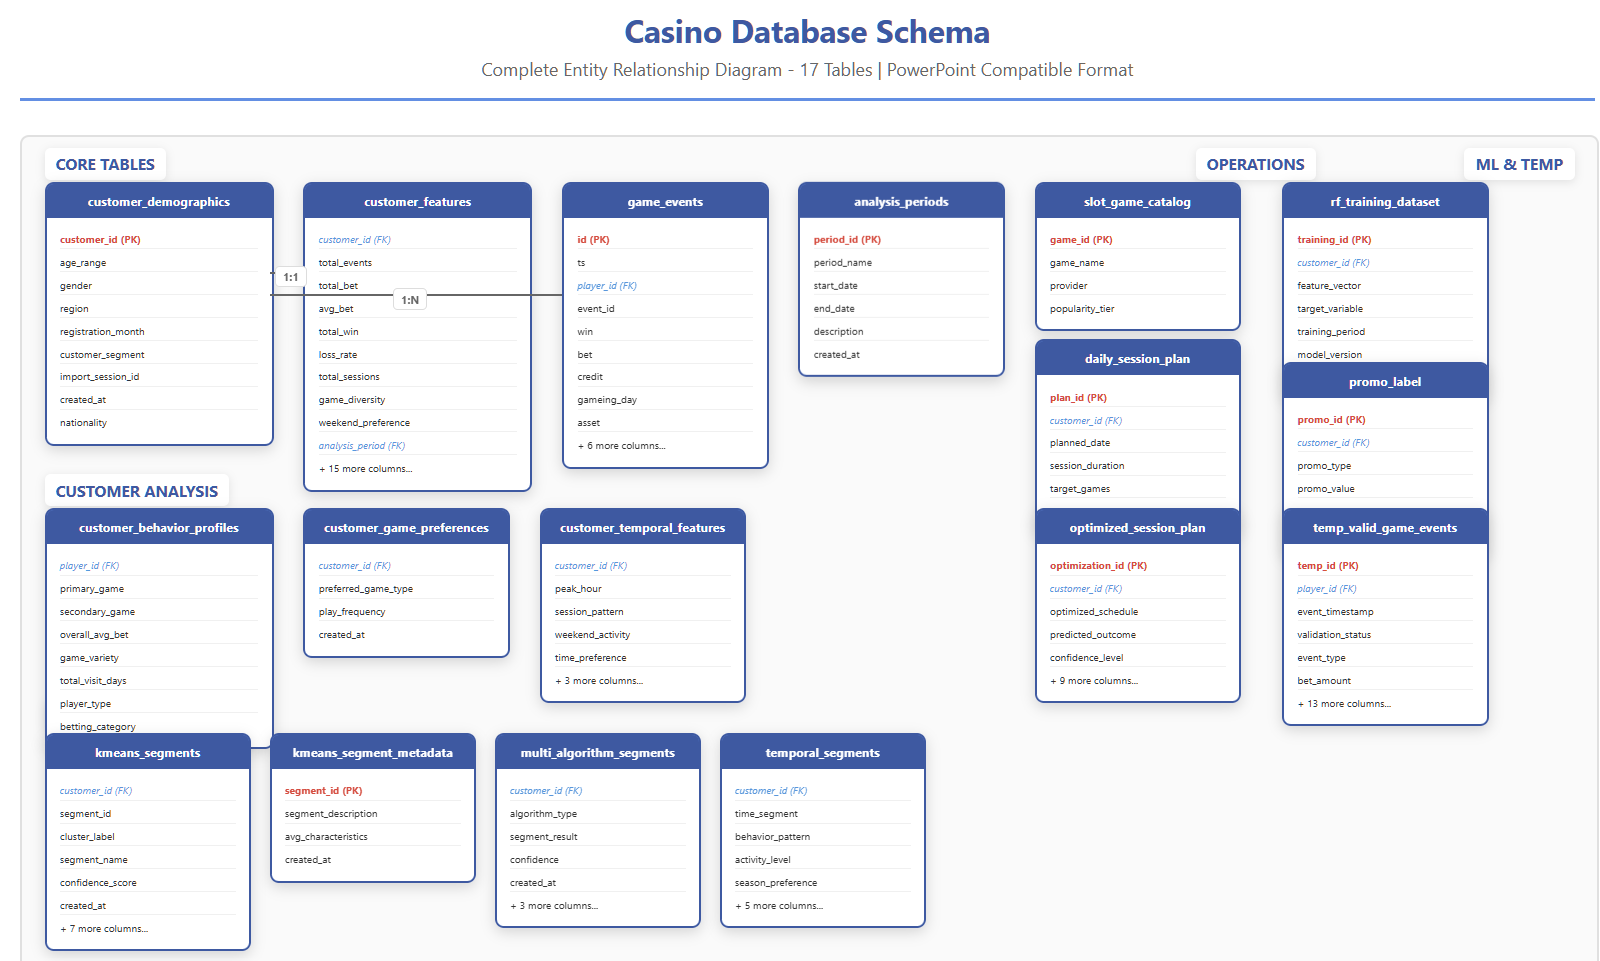
\includegraphics[width=\textwidth]{figures/casino_db_diagram.png}
\caption{PostgreSQL Schema Design for Casino-2 Analytical System}
\label{fig:casino_schema}
\end{figure}


\section{Data Flow and Component Interactions}

The main system is made to work with modular AI processes for dividing customers into groups and making decisions about promotions.  So, the internal data flow links preprocessing, feature extraction, model inference, and API contact parts in a way that can be repeated and is aware of audits.

\subsection{Pipeline Execution via \texttt{main\_pipeline.py}}

At the center of execution is \texttt{main\_pipeline.py}, a callable script that orchestrates the comprehensive data pipeline. It retrieves pre-defined analysis periods, fetches raw data from PostgreSQL, executes feature engineering functions, trains models as required, and stores predictions in the database.  The conditional logic of this module allows for the independent or batch activation of pipeline phases, such as KMeans or Random Forest, across many periods.

\subsection{Behavioural Segmentation with \texttt{segmentation.py}}

The \texttt{segmentation.py} module implements K-Means clustering based on engineered behavioural features. This includes:

\begin{itemize}
    \item Loading clean features from the database for a defined period
    \item Applying standardisation and cluster optimisation heuristics
    \item Mapping clusters into human-readable business labels (Casual, Roller, High Value players)
    \item Writing outputs to \texttt{casino\_data.kmeans\_segments} with versioning
\end{itemize}

It also contains rules and restrictions to exclude outliers or corrupted information (e.g., improper age or null sessions).  The ultimate cluster metadata is retained in \texttt{kmeans\_segment\_metadata} and periodically refreshed to support downstream analytics.

\subsection{Promotional Inference with \texttt{rf\_training.py}}

The \texttt{rf\_training.py} script serves as a supervised learning module for predicting promotional targeting based on segment-specific and behavioural features. Its structure includes:

\begin{itemize}
    \item Stratified sampling and GroupKFold cross-validation
    \item Optional hyperparameter tuning for reproducibility
    \item Integration of probabilistic labelling (e.g., Low, Medium, High impact)
    \item Saving trained models in Pickle format with logs in \texttt{academic\_audit}
\end{itemize}

The outputs of the Random Forest are evaluated using performance metrics and archived for subsequent A/B testing or CRM based simulations.

\subsection{CRM Interaction via RESTful API}

The prediction system is accessible through a FastAPI interface, if required, allowing CRM employees to retrieve segment labels and promotional recommendations for specific clients.  API endpoints are subject to rate limitations and are monitored for audit purposes.  All requests are processed through a logging layer that records timestamps, input parameters, and inference metadata according to the  \texttt{academic\_audit} schema.

\subsection{Component Map Overview}

\begin{itemize}
    \item \texttt{main\_pipeline.py} \textendash{} Central orchestrator for multi-period processing
    \item \texttt{feature\_engineering.py} \textendash{} Extracts features like volatility, recency, and loss chasing
    \item \texttt{segmentation.py} \textendash{} Applies KMeans clustering and stores segments with version control
    \item \texttt{rf\_training.py} \textendash{} Trains Random Forest model and logs artefacts
    \item \texttt{api.py} \textendash{} FastAPI interface for CRM-facing decision retrieval
    \item \texttt{db\_connector.py} \textendash{} Handles PostgreSQL interactions securely
\end{itemize}

This modular configuration ensures that any component can be evaluated, enhanced, or changed freely, allowing persistent scalability and scholarly reproducibility.

%-------------------------------------------------------------------------------

\subsection{AI Modelling and Inference}
\label{sec:ai_modelling_inference}

The modelling component of the Casino AI system is structured as a two-stage machine learning pipeline consisting of unsupervised segmentation and supervised promotional prediction. This pipeline was initially developed under a proof-of-concept prototype called \textbf{Casino-1}, using synthetically generated slot machine data and CRM profiles (approx. 1,5002,000 records). In the production-aligned system \textbf{Casino-2}, the modelling logic was migrated to PostgreSQL-driven modules with anonymised real-world data and audit logging.

\subsubsection*{Behavioural Segmentation (K-Means)}

In Casino-1, segmentation was performed via the \texttt{train\_kmeans.py} module, which clusters customers into three behavioural groups based on engineered features including \texttt{avg\_loss}, \texttt{RTP}, \texttt{session\_duration}, and \texttt{zone\_diversity}, derived from preprocessed slot activity logs. Outputs were visualised in matplotlib-based diagrams (see Figure~\ref{fig:casino1_segmentation}) and stored as \texttt{labeled\_customer\_dataset.csv}. Segment labels were mapped into business-relevant profiles (e.g., Casual, Regular, High Roller).

\begin{figure}[H]
\centering
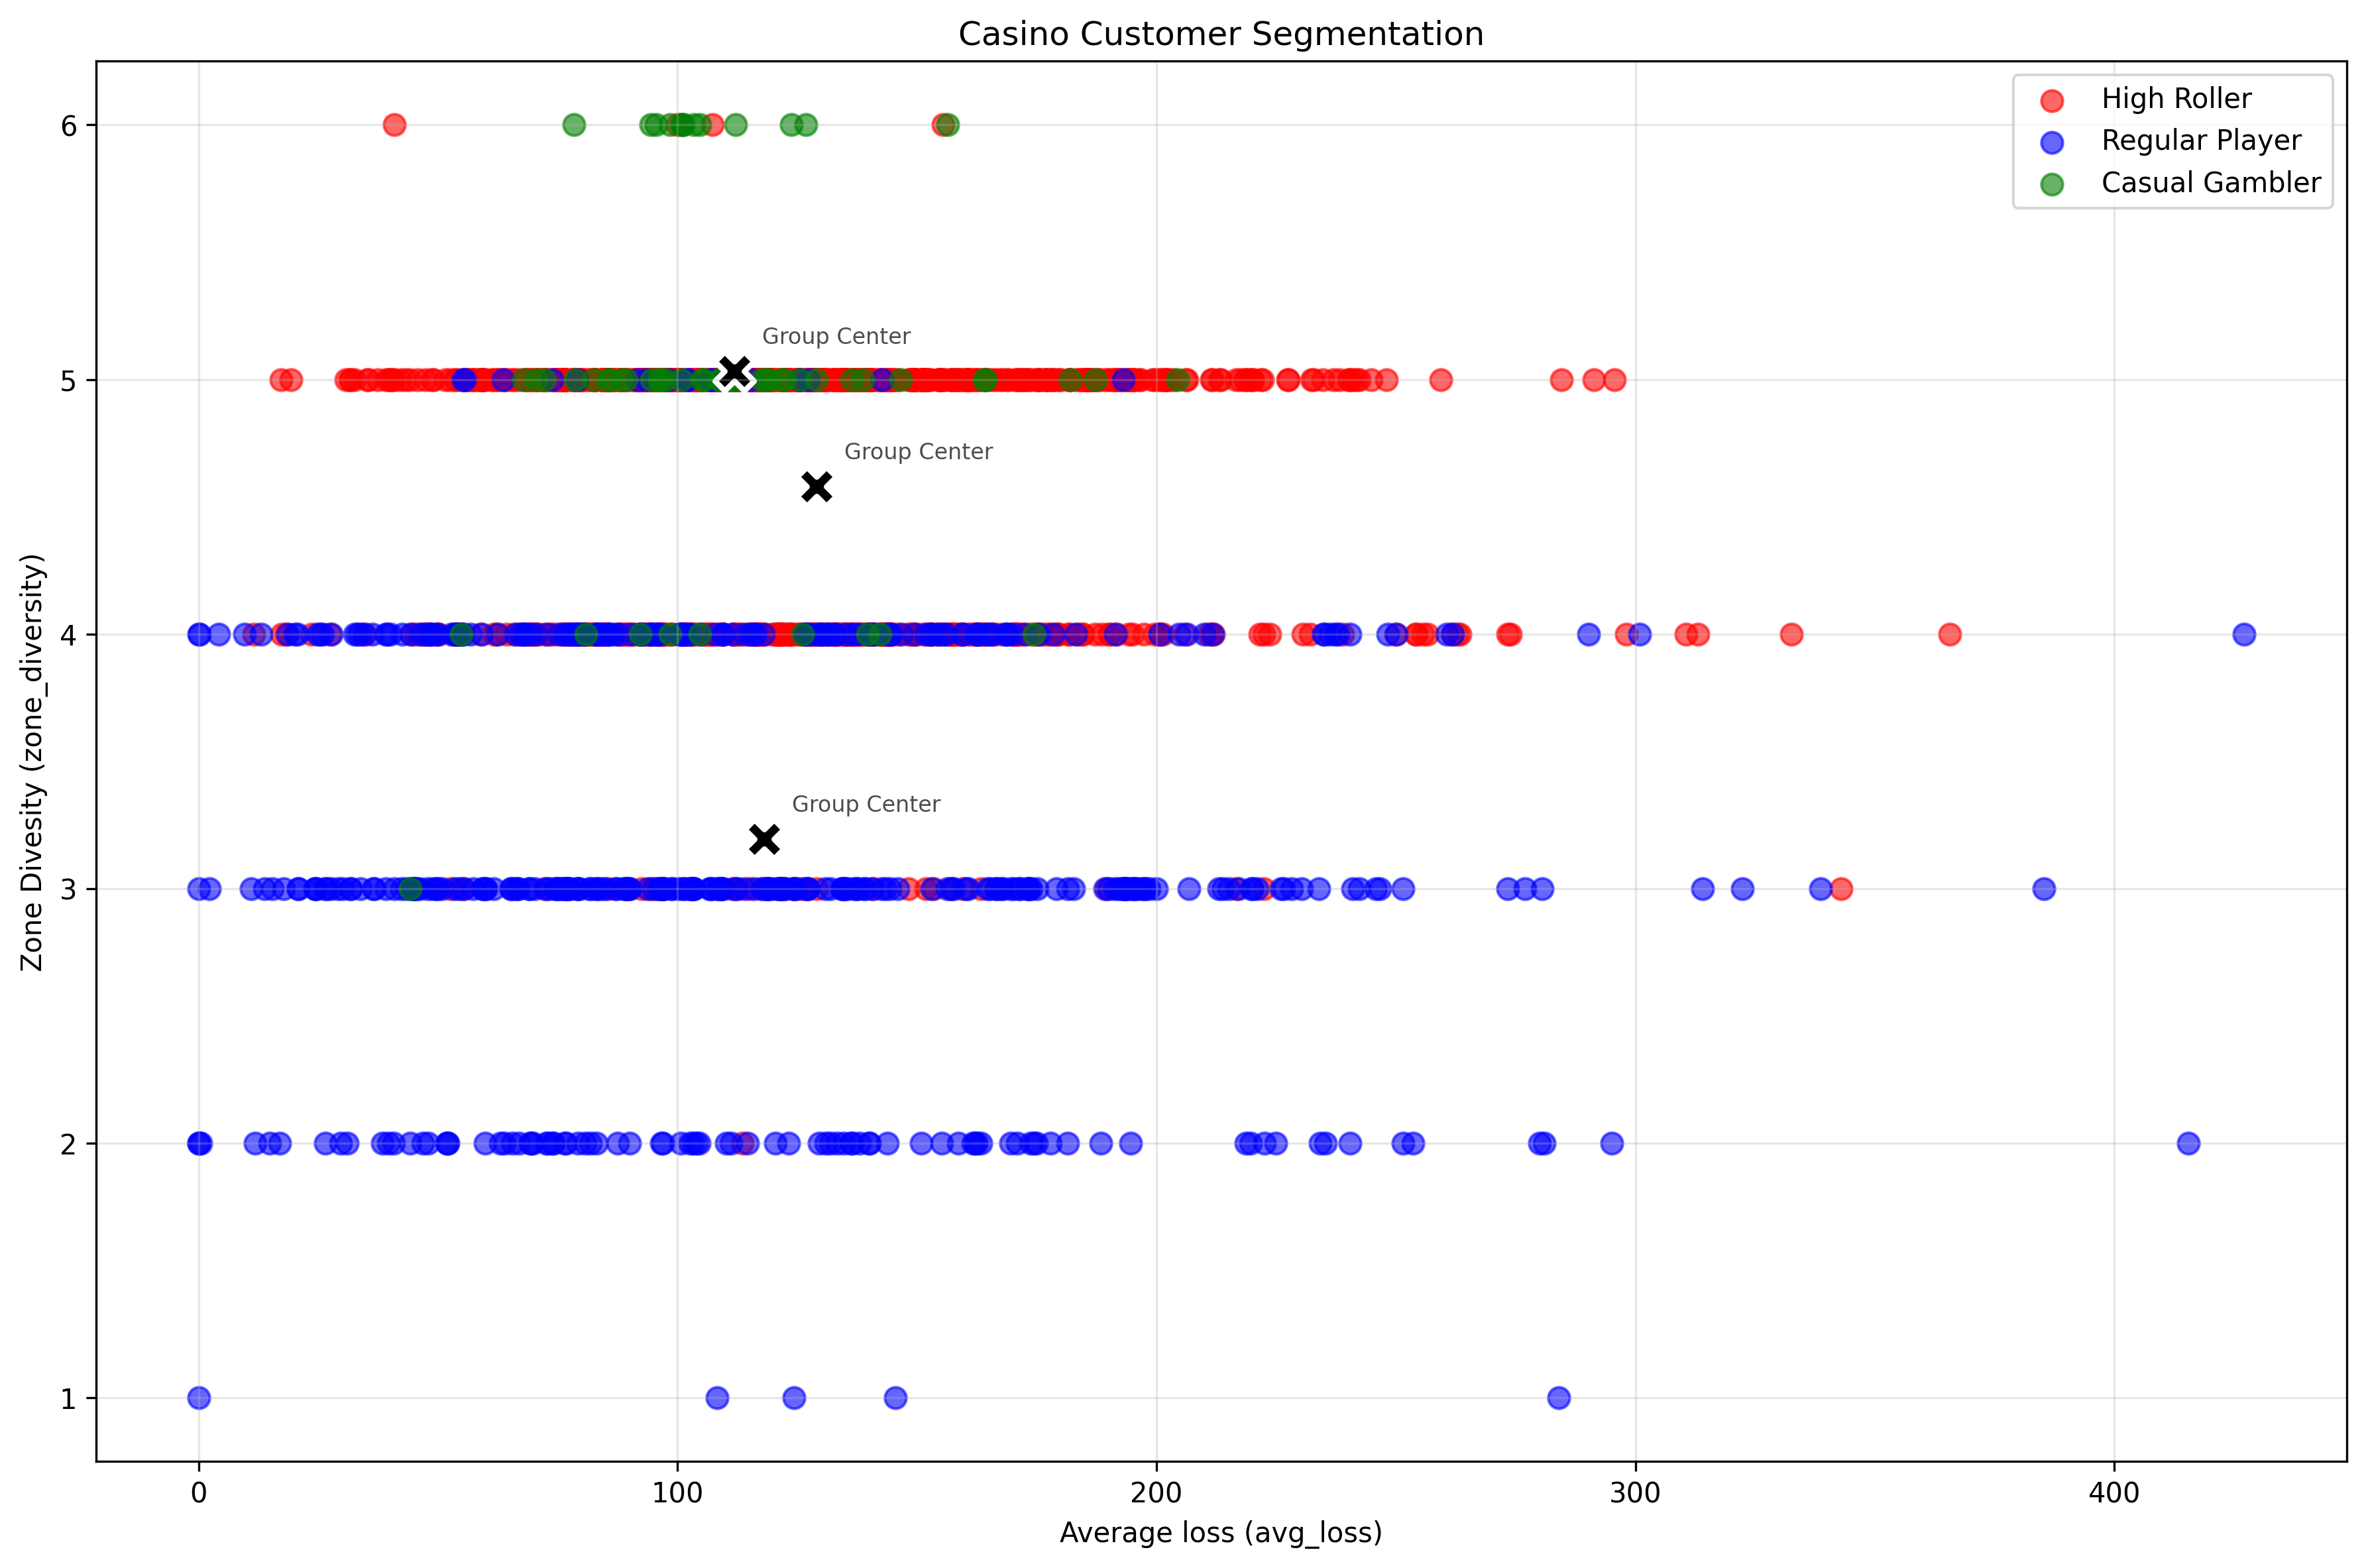
\includegraphics[width=0.8\textwidth]{figures/segmentation_analysis.png}
\caption{K-Means segmentation visualisation for Casino-1 dataset.}
\label{fig:casino1_segmentation}
\end{figure}

In Casino-2, the segmentation task was modularised and adapted to run on structured PostgreSQL tables. Multiple clustering algorithms including DBSCAN and Gaussian Mixture Models were also evaluated using the \texttt{multi\_algorithm\_segments} schema. Each segmentation task is linked to an \texttt{analysis\_period}, enabling longitudinal tracking (e.g., 2022-H1 to 2023-H2).

\subsubsection*{Promotional Prediction (Random Forest)}

The Casino-1 classifier (\texttt{random\_forest\_model.py}) used the segment outputs and CRM feedback as input, training a Random Forest model to predict likelihood of promotional response. The script included grid search, 5-fold cross-validation, confusion matrix visualisation (Figure~\ref{fig:confusion_matrix}), and feature importance analysis (Figure~\ref{fig:feature-importance}). All outputs were saved in JSON and image formats for interpretation.

\begin{figure}[H]
\centering
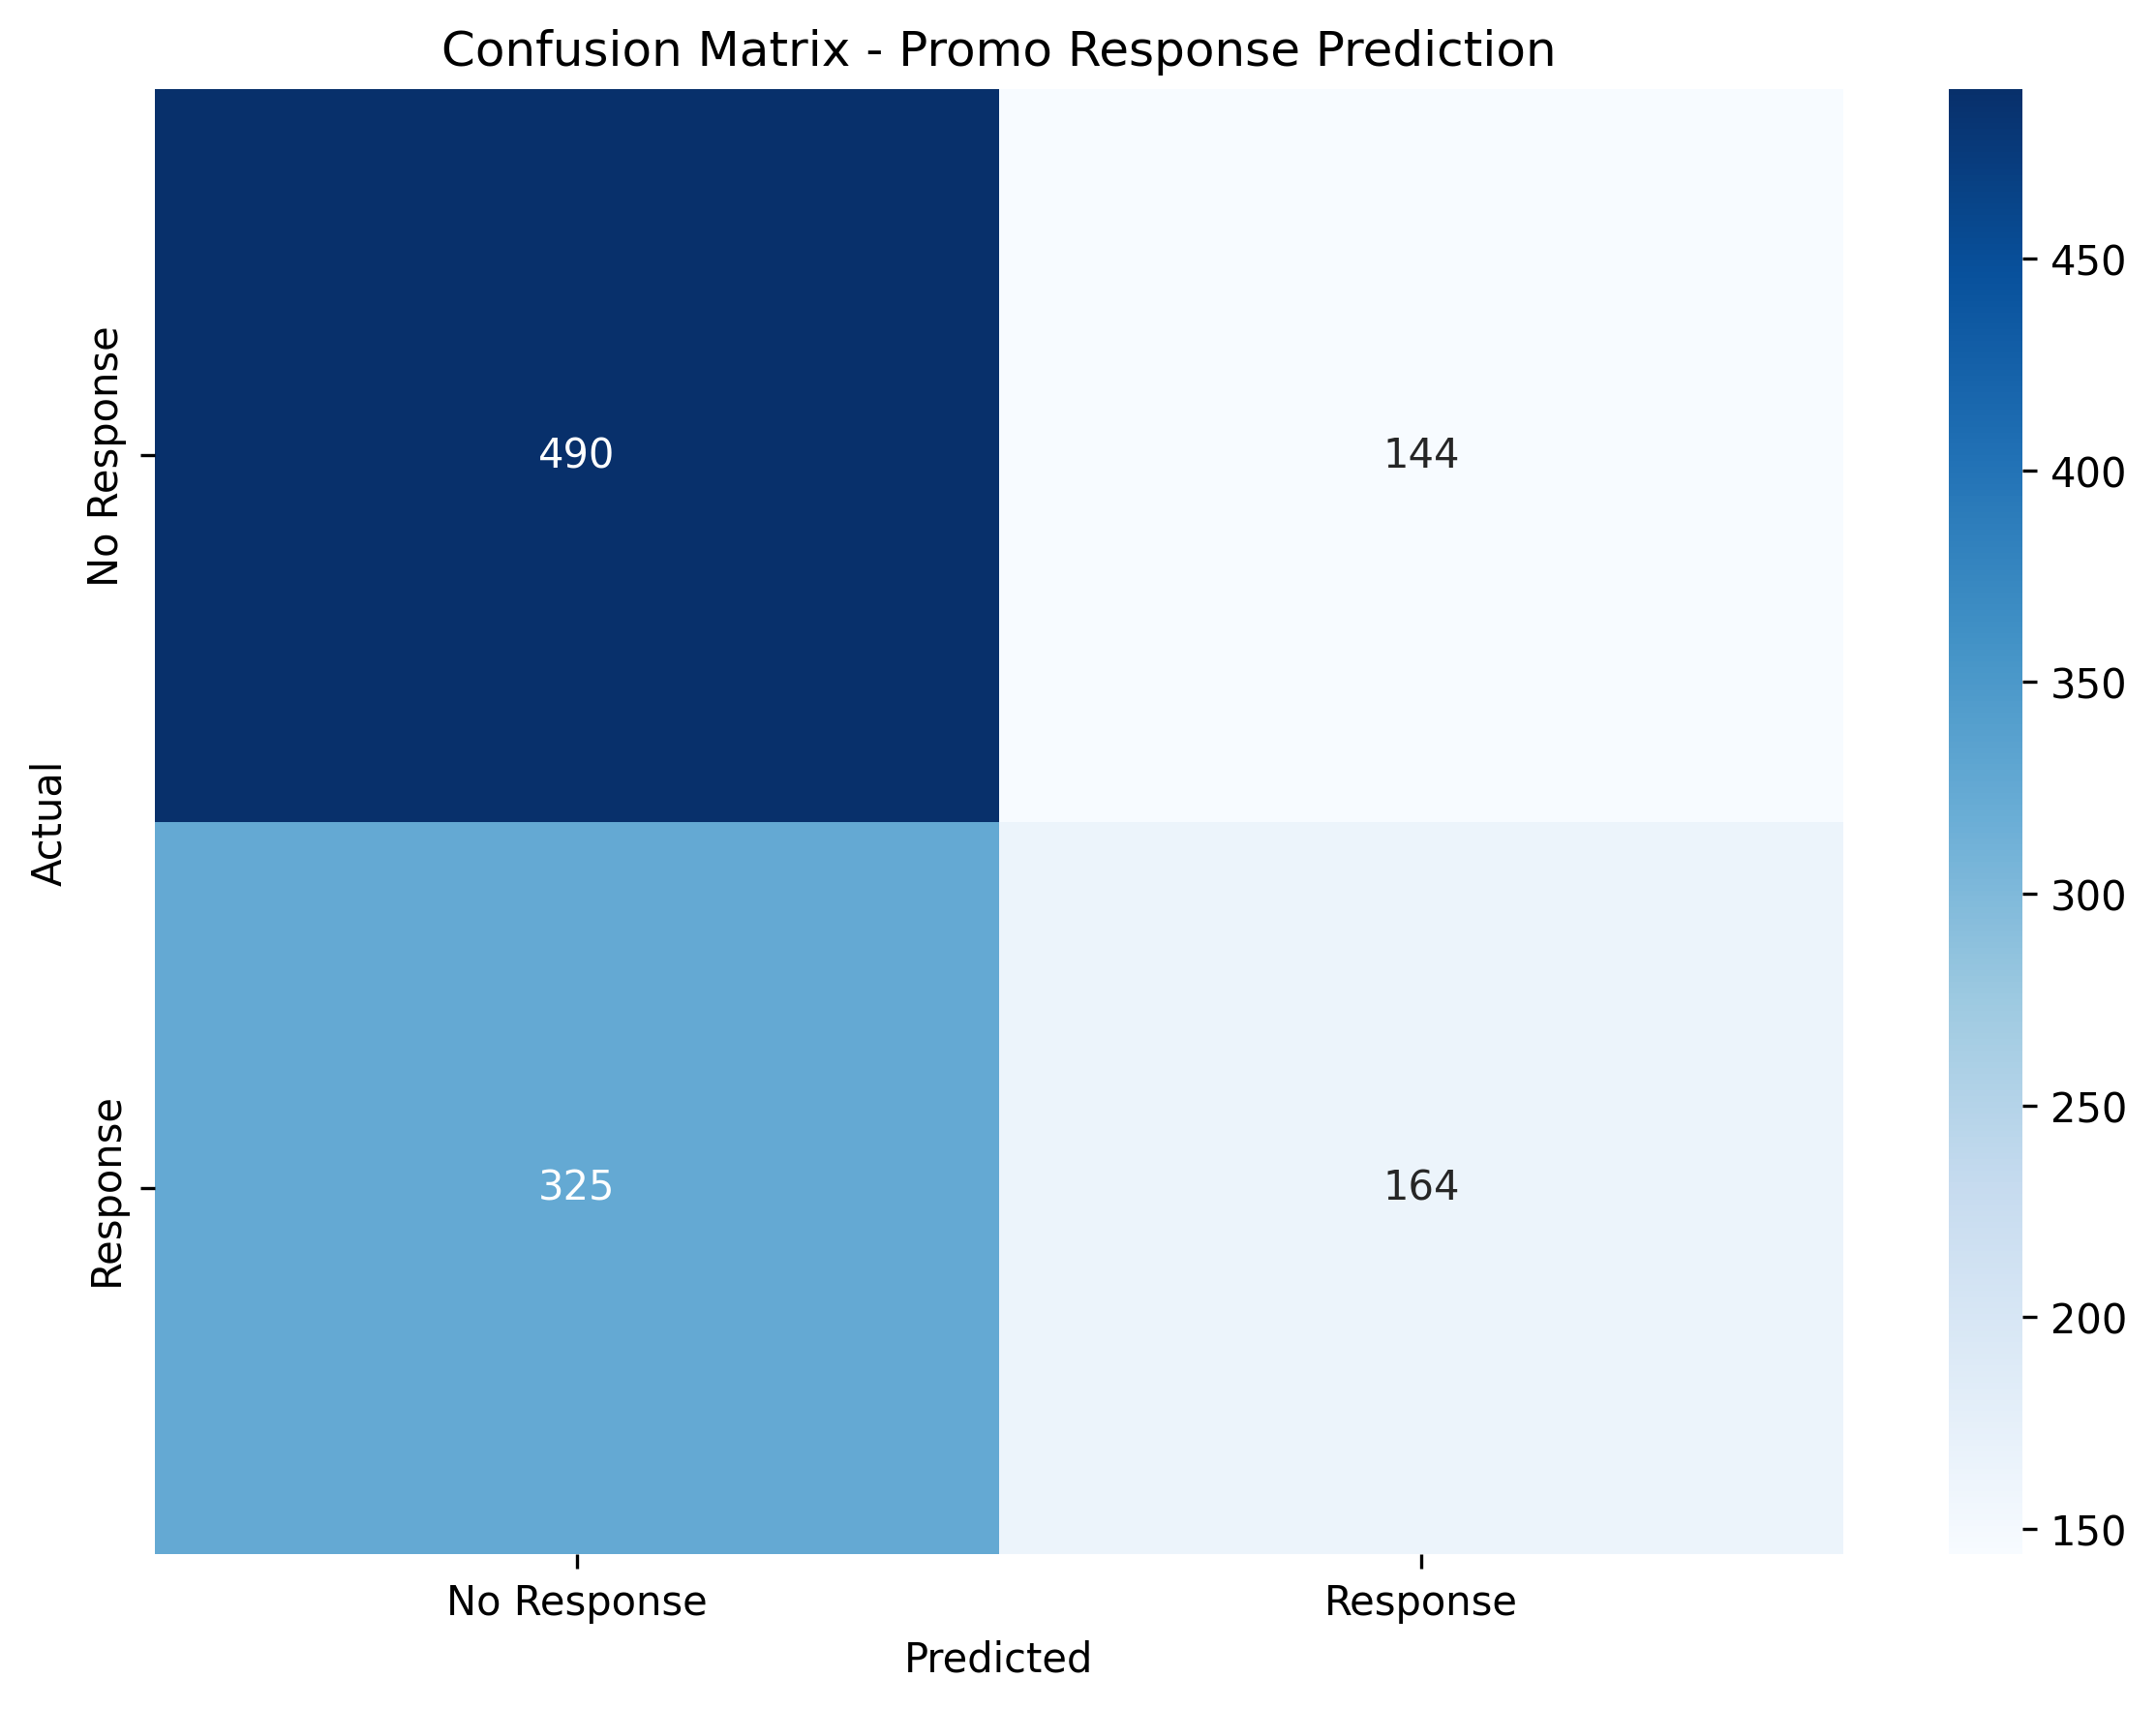
\includegraphics[width=0.8\textwidth]{figures/confusion_matrix.png}
\caption{Confusion Matrix Visualisation and Promo Response.}
\label{fig:confusion_matrix}
\end{figure}

\begin{figure}[H]
\centering
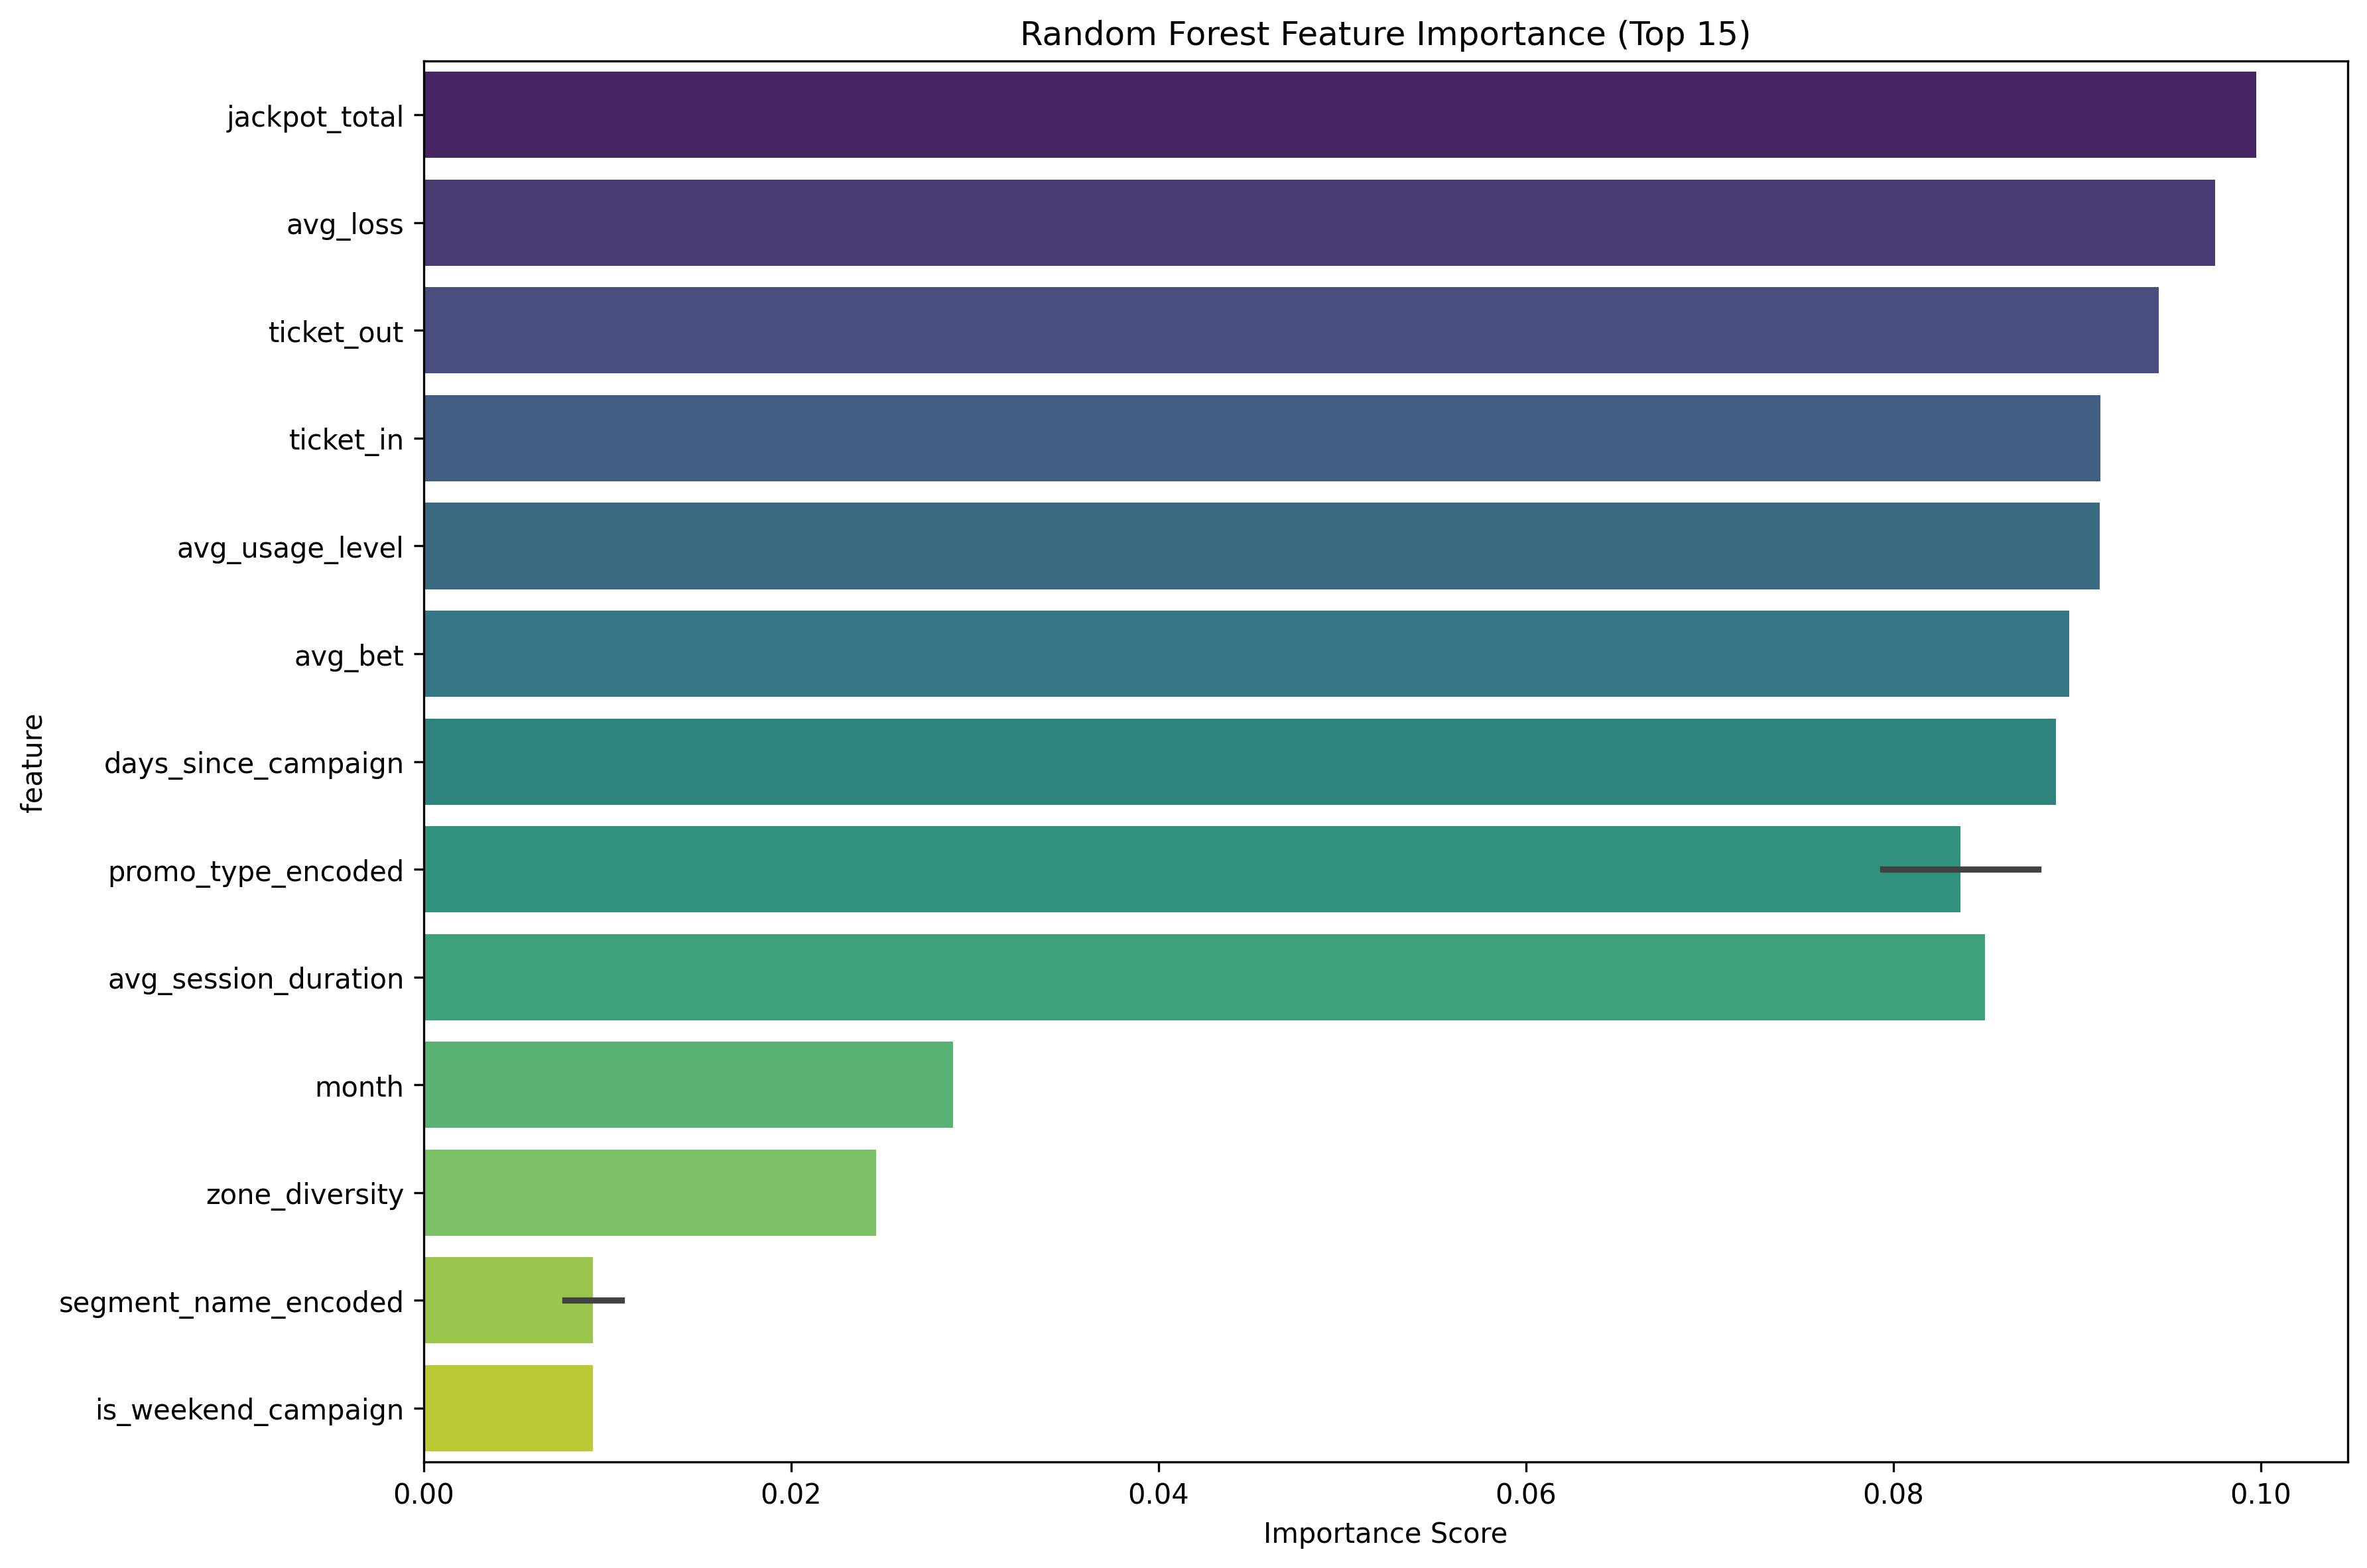
\includegraphics[width=0.8\textwidth]{figures/feature_importance.png}
\caption{Feature Importance Scores from Random Forest Model.}
\label{fig:feature-importance}
\end{figure}

Casino-2 transitioned this pipeline into fully auditable components, applying segment-based labelling and promotion flag harmonisation using domain-informed thresholds. Multiple modules such as \texttt{robust\_rf\_training\_major\_fix.py} and \texttt{enhanced\_rf\_promotion\_model.py} improved class balance, reproducibility, and cross-period generalisation.

Training was conducted independently on four half-year periods (2022-H1, 2022-H2, 2023-H1, 2023-H2) to detect seasonality and behavioural shifts. Feature importance scores and top predictive indicators (e.g., session volatility, bet trend ratio, zone diversity) were tracked across all model runs.


\subsubsection*{FastAPI Exposure and CRM Access}

In all settings, the prediction engine was provided over RESTful API endpoints to help with promotional decision-making. In \textbf{Casino-1}, this was implemented through a  minimal Python API prototype (\texttt{main.py}), It used matplotlib charts to illustrate results after applying a pre-trained model to synthetic customer features supplied from CSV. Quick testing of inference logic and display of results was made possible by the prototype.

In \textbf{Casino-2}, the system was upgraded into a production-aligned FastAPI architecture. Endpoints such as \texttt{/segment} and \texttt{/promotion} get real-time information about customers from the PostgreSQL database, use persistent models to make predictions on demand, and send results in JSON format to outside CRM systems.  A separate model register keeps track of model versions and performance information.

All prediction outputs are stored under the \texttt{academic\_audit} schema with associated timestamps, segment decisions, and promo response probabilities. This setup enables downstream evaluation, future A/B testing, and integration of CRM feedback loops into retraining cycles.

%%%%%%%%%%%%%%%%%%%%%%%%%%%%%%%%%%%%%%%%%%%%%%%%%%%%%%%%%%%%%%%%%%%%%%%%%%%%%%%%
%%%%%%%%%%%%%%%%%%%%%%%%%%%%%%%%%%%%%%%%%%%%%%%%%%%%%%%%%%%%%%%%%%%%%%%%%%%%%%%%

\chapter{Implementation and Testing}

This chapter defines the practical execution of the Casino AI system, comprising data ingestion, feature computation, machine learning model creation, and evaluation.  The emphasis is on converting design elements into functional modules, integrating with PostgreSQL, and facilitating real-time communication through RESTful APIs.  Testing protocols were implemented to evaluate functional accuracy, consistency of forecasts over time, and the auditability of system conclusions.

The execution occurred in two primary phases:

\begin{itemize}
    \item \textbf{Casino-1:} A proof-of-concept environment using synthetic data (1,500–2,000 entries), tested locally with CSV-based inputs, matplotlib visualisations, and lightweight REST APIs via Flask.
    \item \textbf{Casino-2:} The production-aligned academic pipeline operating on PostgreSQL, with modular AI scripts, FastAPI endpoints, feature versioning, and anonymised real casino data spanning four analysis periods (2022-H1 to 2023-H2).
\end{itemize}

The codebase was managed under a structured repository with \texttt{src/}, \texttt{models/}, \texttt{schemas/}, and \texttt{academic/} folders. Each module was iteratively tested, ensuring reproducibility and compliance with the University's ethical approval framework (Ref: 10351-12382).

\section{System Setup and Technologies}
\label{sec:system_setup}

The development and deployment of the Casino AI framework was conducted through a modular and version-controlled environment. This environment was shared between the initial prototype (Casino-1) and the production-aligned academic system (Casino-2). Key technologies included:

\begin{itemize}
    \item \textbf{Python 3.11:} \textit{(Both systems)} Served as the core programming language for data processing, modelling, and automation. Scripts were developed under modular structures using OOP, pandas, scikit-learn, and joblib.

    \item \textbf{PostgreSQL 14:} \textit{(Casino-2 only)} Provided the foundation for the relational database by handling information such as user profiles, game histories, feature tables, and model descriptions.  Anonymisation and performance indexing were applied to all schemas and tables.

    \item \textbf{Docker + Docker Compose:} \textit{(Casino-2 only)} Ensured  PostgreSQL, API services, and Python scripts were deployed in a controlled academic environment in a containerised and repeatable manner.

    \item \textbf{FastAPI:} \textit{(Casino-1 prototype and partially Casino-2)} Whereas Casino-1 used local property files as input, Casino-2 used the registry to get installed models and PostgreSQL to retrieve real-time properties. Although complete CRM connection was not developed in Casino-2 due to scope constraints, RF and K-means results were made available for querying from the database as segmentation and promotion suggestion data.

    \item \textbf{VS Code + Git:} \textit{(Both systems)} Used as the main IDE and version control system so that work can be copied in the educational environment.  It was made possible to sync documents, code, and experiments with GitHub.

    \item \textbf{Matplotlib + Seaborn:} \textit{(Casino-1 only)} Useful for visualisations such as confusion matrix structures, clustering plots, and feature importances.

    \item \textbf{Ethical Audit Trail:} \textit{(Casino-2 only)} Metadata logs, model outputs, and feature importances were saved into the \texttt{academic\_audit} schema to ensure compliance with Bath University ethics approval (Ref: 10351-12382).

\end{itemize}

All components were validated across four analytical periods: \textbf{2022-H1}, \textbf{2022-H2}, \textbf{2023-H1}, and \textbf{2023-H2}. The transition from Casino-1 to Casino-2 indicated a movement from synthetic datasets to real anonymised records, simplifying replicable academic assessment along with improving model reliability.

\section{System Design Evolution}
\label{sec:system_design_evolution}

The design of the Casino AI system was intentionally divided into two phases: \textbf{Casino-1} and \textbf{Casino-2},every part of the development lifecycle has a unique role.  Considerations of an ethical, technical, and administrative nature all contributed to the decision to employ a dual-structure method.

As an exploratory prototype, Casino-1 allowed for early testing of prediction and clustering algorithms in a non-sensitive, risk-free context.  All of the data utilised in Casino-1, including sysnthetic profiles and simulated slot machine logs, was artificially manufactured because official ethical permission was not obtained at beginning of the project.  Without worrying about data privacy issues or non-compliance with regulations, this setting offered a secure platform for assessing the performance of models like Random Forest for promotional prediction and K-Means for segmentation.

The experiment moved to Casino-2, an academic setting that is completely anonymous and aligned with production, after an ethical permit was granted (Ref: 10351-12382). During this stage, a PostgreSQL-backed architecture was built using processed, transformed, and integrated real-world slot data. As a result of this change, additional complications, such as inconsistent \texttt{player\_id} formats, missing zone information, and the necessity to apply compliant anonymisation strategies. Despite these challenges, the transition to real data supported enhanced model evaluation, replicability, and continuous evaluation across four specified periods (2022-H1 to 2023-H2).

This dual-phase method was both ethically essential and technically advantageous.  It facilitated swift iteration and model enhancement in Casino-1, while guaranteeing that Casino-2 maintained academic seriousness, auditability, and the ability to be general. The transition from synthetic to real information indicates a methodological dedication to ethical AI research and a practical approach to feasible intelligence in regulated sectors like casino operations.


\subsection{Development Environment and Tools}

A dual-phase architectural methodology, dependent upon data availability constraints and ethical approval requirements, was employed to construct the system.  While awaiting regulatory authorisation to access real casino data, a proof-of-concept environment designated as \textbf{Casino-1} was established utilising fabricated CRM profiles and digitally generated data.   The simulated environment phase facilitated early testing of clustering and predictive modelling techniques (K-Means, Random Forest), which enhanced and clarified the fundamental concept.

Once ethics approval was granted (Ref: 10351-12382), the full system—\textbf{Casino-2}—was implemented using anonymised real-world data in a PostgreSQL-backed modular pipeline. The transition from synthetic to production-ready data structures presented various challenges, including defective or absent \texttt{zone} data and inconsistencies \texttt{player\_id} formats. Critical data integrity issues were mitigated by enforcing \texttt{BIGINT} conversions, applying regular expressions for ID validation, and generating missing demographic fields using the syntethic data library. These steps were crucial for the consistency of AI pipelines and compliance to academic standards.

\begin{quote}
The implementation of a two-stage strategy was both pragmatic and ethically vital, with Casino-1 functioning as the logical testing platform and Casino-2 as the academic deployment platform.   In addition to ensuring compliant research, it provided rapid insights into consumer segmentation and promotional modelling procedures.
\end{quote}

\subsection{Transitioning from Synthetic to Real Data}

The development process started with a synthetic dataset simulation (Casino-1) to prototype segmentation and prediction logic while simultaneously anticipating formal ethics approval.  Real-world data pipelines (Casino-2) were constructed and deployed in response to the approval (Ref: 10351-12382), which enabled the use of anonymised operational data from the Imperial Palace Casino to conduct comprehensive behavioural modelling.

The initial modelling experiments were conducted on \textbf{Casino-1}, a synthetic dataset comprising approximately 1,500–2,000 customer records. This environment was critical for prototyping the segmentation logic (via \texttt{train\_kmeans.py}) and promotional prediction model (\texttt{random\_forest\_model.py}), both of which operated on simulated slot sessions and artificial feedback. An ethically-free controlled environment was used to develop evaluation measures, confusion matrices, and feature importances.

Upon ethics approval (Ref: 10351-12382), the system transitioned to the production-aligned \textbf{Casino-2} pipeline. During this stage, real operational obstacles were introduced, including:

\begin{itemize}
  \item \textbf{Data Type Inconsistencies:} The \texttt{player\_id} and \texttt{customer\_id} fields were stored as \texttt{TEXT} in several tables, leading to join failures and NULL propagation in model training queries. A universal conversion to \texttt{BIGINT} was performed to harmonise all references.
  \item \textbf{Zone Information Missingness:} Many session records lacked valid \texttt{zone} identifiers, obstructing features such as zone diversity and heatmap-derived metrics.
  \item \textbf{Uncleaned Foreign Keys:} Several tables, particularly \texttt{game\_events} and \texttt{tito\_transactions}, contained unpaired or inadequate identifiers, requiring regular expression filters and additional processes.
\end{itemize}

Despite these challenges, the change maintained the architectural integrity of the Casino-1 prototype.  All pipeline components—segmentation, labelling, training, and exposure—were restructured to enhance auditability, temporal generalisation (2022-H1 to 2023-H2), and compliance with BATH requirements.  Consequently, the system evolved into a scientifically justified framework that connects simulation with real-world modelling.

\subsection{Promotional Targeting Limitations and Validation Strategy}

In the project's initial phase, there was an absence of real-world CRM feedback concerning customer responses to promotions.  As a result, the Random Forest classifier was not trained on real promotional outcomes or acceptance behaviour.  The model was constructed utilising internally derived features, including session volatility, zone diversity, loss-chasing score, and bet trend ratio.  Behavioural signals were derived from the engineered features table and aligned with segment outputs.

 No heuristic or simulated labelling was utilised for promotional response to maintain the academic integrity of the study.  This decision guaranteed that all model outputs were based on behavioural data rather than assumptions.

 Model evaluation utilised standard metrics such as cross-validated accuracy, confusion matrix visualisation, and feature importance analysis.  The results facilitated the evaluation of the reliability of linking customer engagement signals to promotional eligibility, despite the lack of labelled CRM data.  All outputs, including figures and JSON-based logs, were preserved within the \texttt{academic\_audit} schema to facilitate reproducibility and future integration of A/B testing.


\section{Data Preprocessing and Feature Engineering}
\label{sec:data_preprocessing_feature_engineering}

The foundation of the Casino AI pipeline was data preparation, which acted as a link between raw logs and datasets that were ready for modelling.  Preprocessing procedures were used in both the Casino-1 and Casino-2 settings, although there were notable differences in phase-to-phase variations in complexity and data integrity.

\subsection*{Casino-1 Feature Engineering}

In Casino-1, features were derived from synthetic slot session logs and some of CRM fields. Modules such as \texttt{train\_kmeans.py} and \texttt{random\_forest\_model.py} included internal logic for computing key behavioural indicators:

\begin{itemize}
  \item \texttt{avg\_loss} – average loss per session
  \item \texttt{session\_duration} – mean duration of each slot session
  \item \texttt{RTP} – return-to-player ratio over session windows
  \item \texttt{zone\_diversity} – number of unique slot machine zones visited
\end{itemize}

These engineered features were statically extracted from CSV files and passed directly into clustering and classification models. Labeling for promotional response was simulated using heuristics based on usage frequency and segment type.

\subsection{Casino-2 Feature Pipeline}

In Casino-2, preprocessing was structured and developed into a multi-phase, verifiable pipeline.  Enhancements were implemented applying PostgreSQL views and Python-based transforms.

\begin{itemize}
  \item \textbf{BIGINT conversion}: Ensured consistent identifier formats across \texttt{player\_id} and \texttt{customer\_id}.
  \item \textbf{Null and Dirty Value Cleansing}: Detected and removed malformed session records and unmatched foreign keys using regex filters.
  \item \textbf{Loss-Chasing Score}: Introduced a custom metric to capture compulsive betting patterns based on volatility thresholds.
  \item \textbf{Temporal Features}: Computed metrics over rolling time windows, including \texttt{sessions\_last\_30d} and \texttt{bet\_trend\_ratio}.
  \item \textbf{Anonymised Demographics}: Where CRM fields were absent, demographic fields such as age and nationality were synthetically filled using the Faker library, maintaining GDPR compliance.
\end{itemize}

All features were stored in the \texttt{casino\_data.customer\_features} table, joined with segmentation and model input pipelines. The feature pipeline supported both batch and real-time retrieving modes, enabling flexible experimentation and CRM integration.

\subsection*{Versioning and Auditability}

Each version of the feature set was logged via the \texttt{academic\_audit} schema with timestamps, source query hashes, and preprocessing notes. This ensured that model training could be repeated or rolled back as needed, aligning with academic integrity and reproducibility requirements.

\subsection{Feature Design for Segmentation}

The segmentation phase relied heavily on features that reflect underlying behavioural diversity among players. After extensive correlation testing and practical evaluation, the following features were prioritised:

\begin{itemize}
  \item \texttt{avg\_loss}: Indicates monetary intensity of a customer’s slot activity.
  \item \texttt{session\_duration\_volatility}: Standard deviation of playtime across sessions, capturing playstyle inconsistency.
  \item \texttt{zone\_diversity}: Number of unique zones visited in a session, suggesting exploration tendency.
  \item \texttt{sessions\_last\_30d}: Count of sessions over the past 30 days, used to detect player engagement trend.
  \item \texttt{bet\_trend\_ratio}: Slope of average bet amount over time, indicative of player risk inclination.
\end{itemize}

K-Means clustering was performed using this feature set, and each data slice (e.g., 2022-H1, 2022-H2) was segmented independently. Label mapping into business-friendly profiles (e.g., Regular, High Roller, At Risk) was handled post-clustering through statistical thresholding and domain-informed heuristics.

\subsection{Feature Design for Promotional Prediction}

The Random Forest classifier required an expanded set of features that included both behavioural and demographic aspects.  Furthermore, the subsequent items were included:

\begin{itemize}
  \item \texttt{loss\_chasing\_score}: Derived using a volatility-weighted aggression metric.
  \item \texttt{customer\_segment}: Imported from previous K-Means results to capture long-term persona.
  \item \texttt{nationality\_group} and \texttt{age\_range}: Derived from CRM or synthetic-based synthetic demographic injection.
  \item \texttt{engagement\_level}: Aggregated score combining recency, frequency, and intensity.
\end{itemize}

These features were designed to align with behavioural dimensions explored in casino marketing literature \citep{Abarbanel2022}, and are further evaluated during model training and validation (Section~\ref{sec:model_training}).

\subsection{Validation through Feature Drift and Importance Scores}

All features were subjected to drift analysis across periods using mean, standard deviation, and entropy tracking. Features exhibiting instability or period bias were dropped or transformed. In final model runs, feature importance graphs were extracted (see Figure~\ref{fig:feature-importance}) and validated against domain expectations. This feature importance plot was generated during early experimentation on the Casino-1 synthetic dataset and is presented for illustrative purposes only. The final production model in Casino-2 uses anonymised real data and generated feature importance scores not shown here.


\subsection{Model Input Preparation}
\label{sec:model_input_preparation}

After the feature engineering was done, model input datasets were made for both the task of segmentation and the task of advertising prediction.  During the preparation part, standards for academic validation were met and consistency, traceability, and alignment were made confident of.

\subsubsection*{Data Joins and Filters}

Records were extracted from the \texttt{casino\_data.customer\_features} table, joined with corresponding segmentation outputs (\texttt{kmeans\_segments}) and, when applicable, promotion labels. Only customers with complete feature vectors and valid anonymised IDs were retained, ensuring a high-quality input set.

\subsubsection*{Label Generation for Promotion Response}

Behavior-informed limits and segment alignment were used to make promotional labels. One example is users in the \texttt{High\_Value} segment who consistently re-engaged were marked as likely to answer. Because real CRM input wasn't available during the model training stage, this heuristic labelling method had to be used.

\subsubsection*{Train-Test Splitting and Balancing}

In order to ensure equal representation across segments and label classes, input datasets were divided using stratified K-fold cross-validation.  To reduce the class inequality in promotion response prediction, more balancing was implemented in Casino-2 using SMOTE analysis and under-sampling approaches.

This was especially effective in improving recall scores for underrepresented classes, a key metric for promotional targeting scenarios \citep{bunkhumpornpat2009tomeklinksmote}.


\paragraph{SMOTE-Based Class Balancing}

SMOTE-based balancing involves the generation of synthetic data points for the minority class to achieve a balanced class distribution, as compared with depending only on duplication or under-sampling methods. This technique improves the learning process by providing the model with an expanded number of representative examples from the under-represented class \citep{chawla2002smote}.

In order to address the imbalance observed in the promotional response labels—where a substantial majority of customers were labelled as \texttt{No Response}—the Synthetic Minority Over-sampling Technique (SMOTE) was employed. SMOTE operates by selecting a sample from the minority class, identifying its nearest neighbours in feature space, and generating new synthetic samples along the line segments joining them. This process enables the creation of diverse, non-redundant instances that represent plausible variations of underrepresented customer behaviour. By applying SMOTE after stratified splitting, the evaluation process preserved statistical validity while avoiding data leakage. This enhanced the model's ability to generalise across behavioural patterns not sufficiently captured by the original training data.

For instance, consider a scenario in which there are 100 users in the minority class labelled as \texttt{High Response}. Simply duplicating these users would risk overfitting the model to known patterns. Instead, SMOTE identifies each user’s nearest neighbours—such as the five closest in the feature space—and generates new, intermediate samples between them. These synthetic instances maintain behavioural plausibility while diversifying the minority class. As a result, the model is trained not only on known examples, but also on variations that may exist in the real world but are not present in the original dataset.

Each stratified split was followed by the exclusive application of SMOTE to the training subset in order to prevent information leaking. Stratified K-Fold cross-validation was subsequently used to the enhanced dataset, maintaining class distribution while ensuring consistent evaluation across folds.


\subsubsection*{Feature Scaling}

Selected features such as \texttt{bet\_trend\_ratio} and \texttt{session\_duration\_volatility} were scaled using conventional normalisation methods. For distance-based algorithms and comparative analysis against models such as SVM and Logistic Regression, this proved crucial.


\subsection{System Pipeline and Feature Computation Architecture}
\label{sec:system_pipeline_feature_architecture}

The implementation of the casino decision-support system required an end-to-end architecture encompassing data integration, feature engineering, segmentation, and supervised learning components. This architecture was developed in alignment with the Casino-2 production-aligned environment, and supported by a PostgreSQL database backend designed to store raw logs, computed features, segment labels, and model outputs.

\paragraph{Feature Engineering and Column Architecture}:

Behavioural and temporal features were engineered to capture nuanced aspects of player activity. These included indicators such as "\texttt{loss\_chasing\_score}, \texttt{bet\_trend\_ratio}, \texttt{session\_duration\_volatility}, \texttt{sessions\_last\_30d}, and \texttt{risk\_score}", among others. Computation pipelines were developed in Python and executed in batch mode, writing results back into dedicated PostgreSQL columns under the \texttt{casino\_data.customer\_features} table. These features were derived through a combination of SQL-based aggregations, temporal windowing, and statistical transformations based on player history logs.

The logic for these metrics was aligned with domain-specific behavioural thresholds. For instance, \texttt{loss\_chasing\_score} was defined using cumulative net losses within a moving time window, whereas \texttt{bet\_trend\_ratio} computed the slope of bet amount trends to detect spikes or downturns. All engineered features were stored in a structured format and indexed by anonymised \texttt{customer\_id} values to ensure auditability and traceability.
\vspace{0.5em}

\paragraph{Rationale Behind Feature Selection}:
Behavioural and temporal features were then engineered to capture nuanced aspects of player activity. These included indicators such as \texttt{loss\_chasing\_score}, \texttt{bet\_trend\_ratio}, \texttt{session\_duration\_volatility}, \texttt{sessions\_last\_30d}, and \texttt{risk\_score}, among others. Computation pipelines were developed in Python and executed in batch mode, writing results back into dedicated PostgreSQL columns under the \texttt{casino\_data.customer\_features} table. These features were derived through a combination of SQL-based aggregations, temporal windowing, and statistical transformations based on player history logs.



\paragraph{Model Pipeline and Training Integration}:
\label{sec:model_training}

The segmentation and prediction modules received the cleaned dataset after feature computation.  The supervised learning datasets were prepared by first applying K-Means clustering to create customer segments, and then merging those segments with the behavioural attributes.  We used segment-specific thresholds to computationally build promotional labels (as outlined in  Appendix~\ref{appendix:validation_rules}) to simulate reasonable responses and attend them to the customers.

The Random Forest classifier was trained using these composite inputs. The full training pipeline was orchestrated via the \texttt{main\_pipeline.py} script, which included data extraction, preprocessing, SMOTE-based resampling, model fitting, and persistence of the trained classifier to a \texttt{.pkl} object. This modular training approach enabled reproducibility and consistent validation via Stratified K-Fold splitting, a cross-validation strategy that preserves the distribution of target classes across all folds to ensure fair evaluation, especially under class imbalance conditions.


\paragraph{System Integration and Execution}:

All core steps — including data access, feature computation, segmentation, and training — were executed within a Dockerised environment for stability and portability. PostgreSQL served as the central data hub, with Python modules reading and writing to feature-specific columns in transactional mode. This setup ensured compatibility with future production deployment and supported analytical traceability during experimental iterations.

As shown in Figure~\ref{fig:casino2_pipeline}, the AI framework integrates PostgreSQL-backed feature computation with SMOTE-enhanced supervised learning under stratified validation constraints.


\begin{figure}[H]
    \centering
    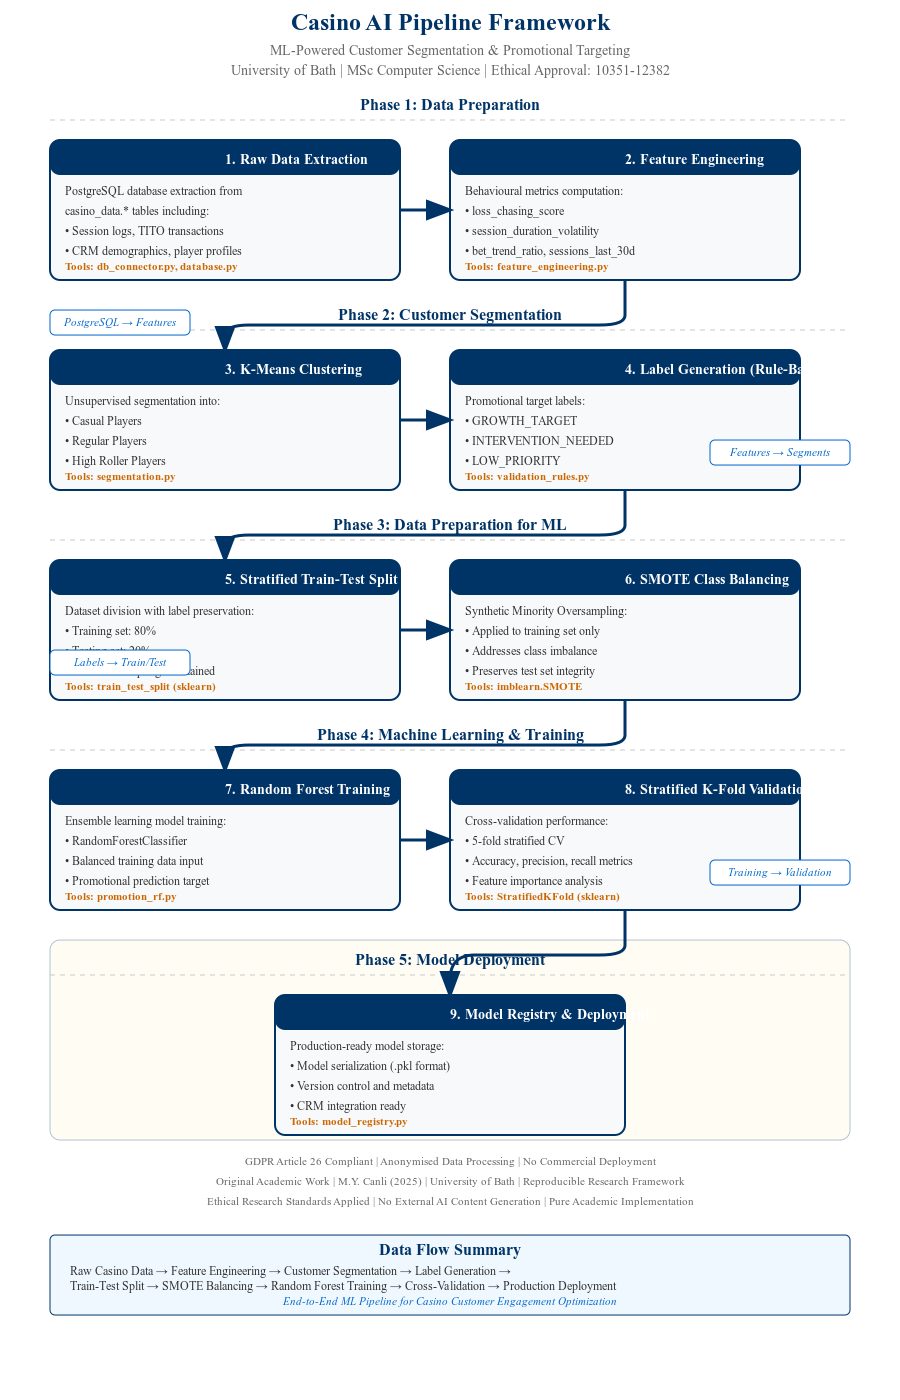
\includegraphics[width=0.95\textwidth]{figures/casino2_pipeline.png}
    \caption{Casino AI Pipeline: ML-Powered Customer Segmentation Framework. This figure summarises the modular end-to-end workflow, integrating unsupervised segmentation, rule-based label generation, SMOTE-enhanced supervised learning, and deployment-ready model serialization.}
    \label{fig:casino2_pipeline}
\end{figure}

The full training and validation flow of the Casino-2 AI framework is summarised in Figure~\ref{fig:casino2_pipeline}, demonstrating each stage from raw data extraction to model deployment.


%%%%%%%%%%%%%%%%%%%%%%%%%%%%%%%%%%%%%%%%%%%%%%%%%%%%%%%%%%%%%%%%%%%%%%%%%%%%%%%%
%%%%%%%%%%%%%%%%%%%%%%%%%%%%%%%%%%%%%%%%%%%%%%%%%%%%%%%%%%%%%%%%%%%%%%%%%%%%%%%%
\chapter{Results}
\label{sec:results}

\section{Overview of Evaluation Strategy}

This chapter evaluates the AI-driven promotional choice system created within the Casino-2 framework.  The system was engineered to produce client segmentations and promotional forecasts for four semiannual periods: 2022-H1, 2022-H2, 2023-H1, and 2023-H2.

To guarantee academic rigour, performance was evaluated by quantitative indicators and visual examination.  The assessment examines client expansion, targeted promotional strategies by segment, temporal shifts in corporate priorities, and the confidence metrics of the Random Forest classifier.  Each figure represents outputs from trained models validated by stratified K-Fold cross-validation on SMOTE-balanced data.

\subsection{Customer Volume and Growth}
\label{sec:customer_growth}

\begin{table}[H]
\centering
\caption{Customer Volume Across Evaluation Periods}
\label{tab:customer_count_by_period}
\begin{tabular}{lrr}
\toprule
\textbf{Period} & \textbf{Customer Count} \\
\midrule
2022-H1 & 2,329 \\
2022-H2 & 3,809 \\
2023-H1 & 6,649 \\
2023-H2 & 15,104 \\
\midrule
\textbf{Total} & \textbf{27,891} \\
\bottomrule
\end{tabular}
\end{table}


The customer base grew significantly across the four evaluation periods. As shown in Figure~\ref{tab:behavioural_stats_by_period}, the system evaluated 2,329 customers in 2022-H1, increasing to over 15,000 in 2023-H2. Data availability enhancements, improved ID matching logic, and the extension of casino activity logs in the production environment are the reasons for this growth.

\noindent
Table~\ref{tab:customer_count_by_period} provides a consolidated view of the system’s performance metrics and prediction outcomes across the four evaluation periods. It visually integrates key dimensions such as customer base expansion, promotion type distribution, prediction confidence evolution, and alignment with business priority categories. 

The AI system's performance was summarised across many temporal dimensions using a unified dashboard.

\begin{figure}[H]
\centering
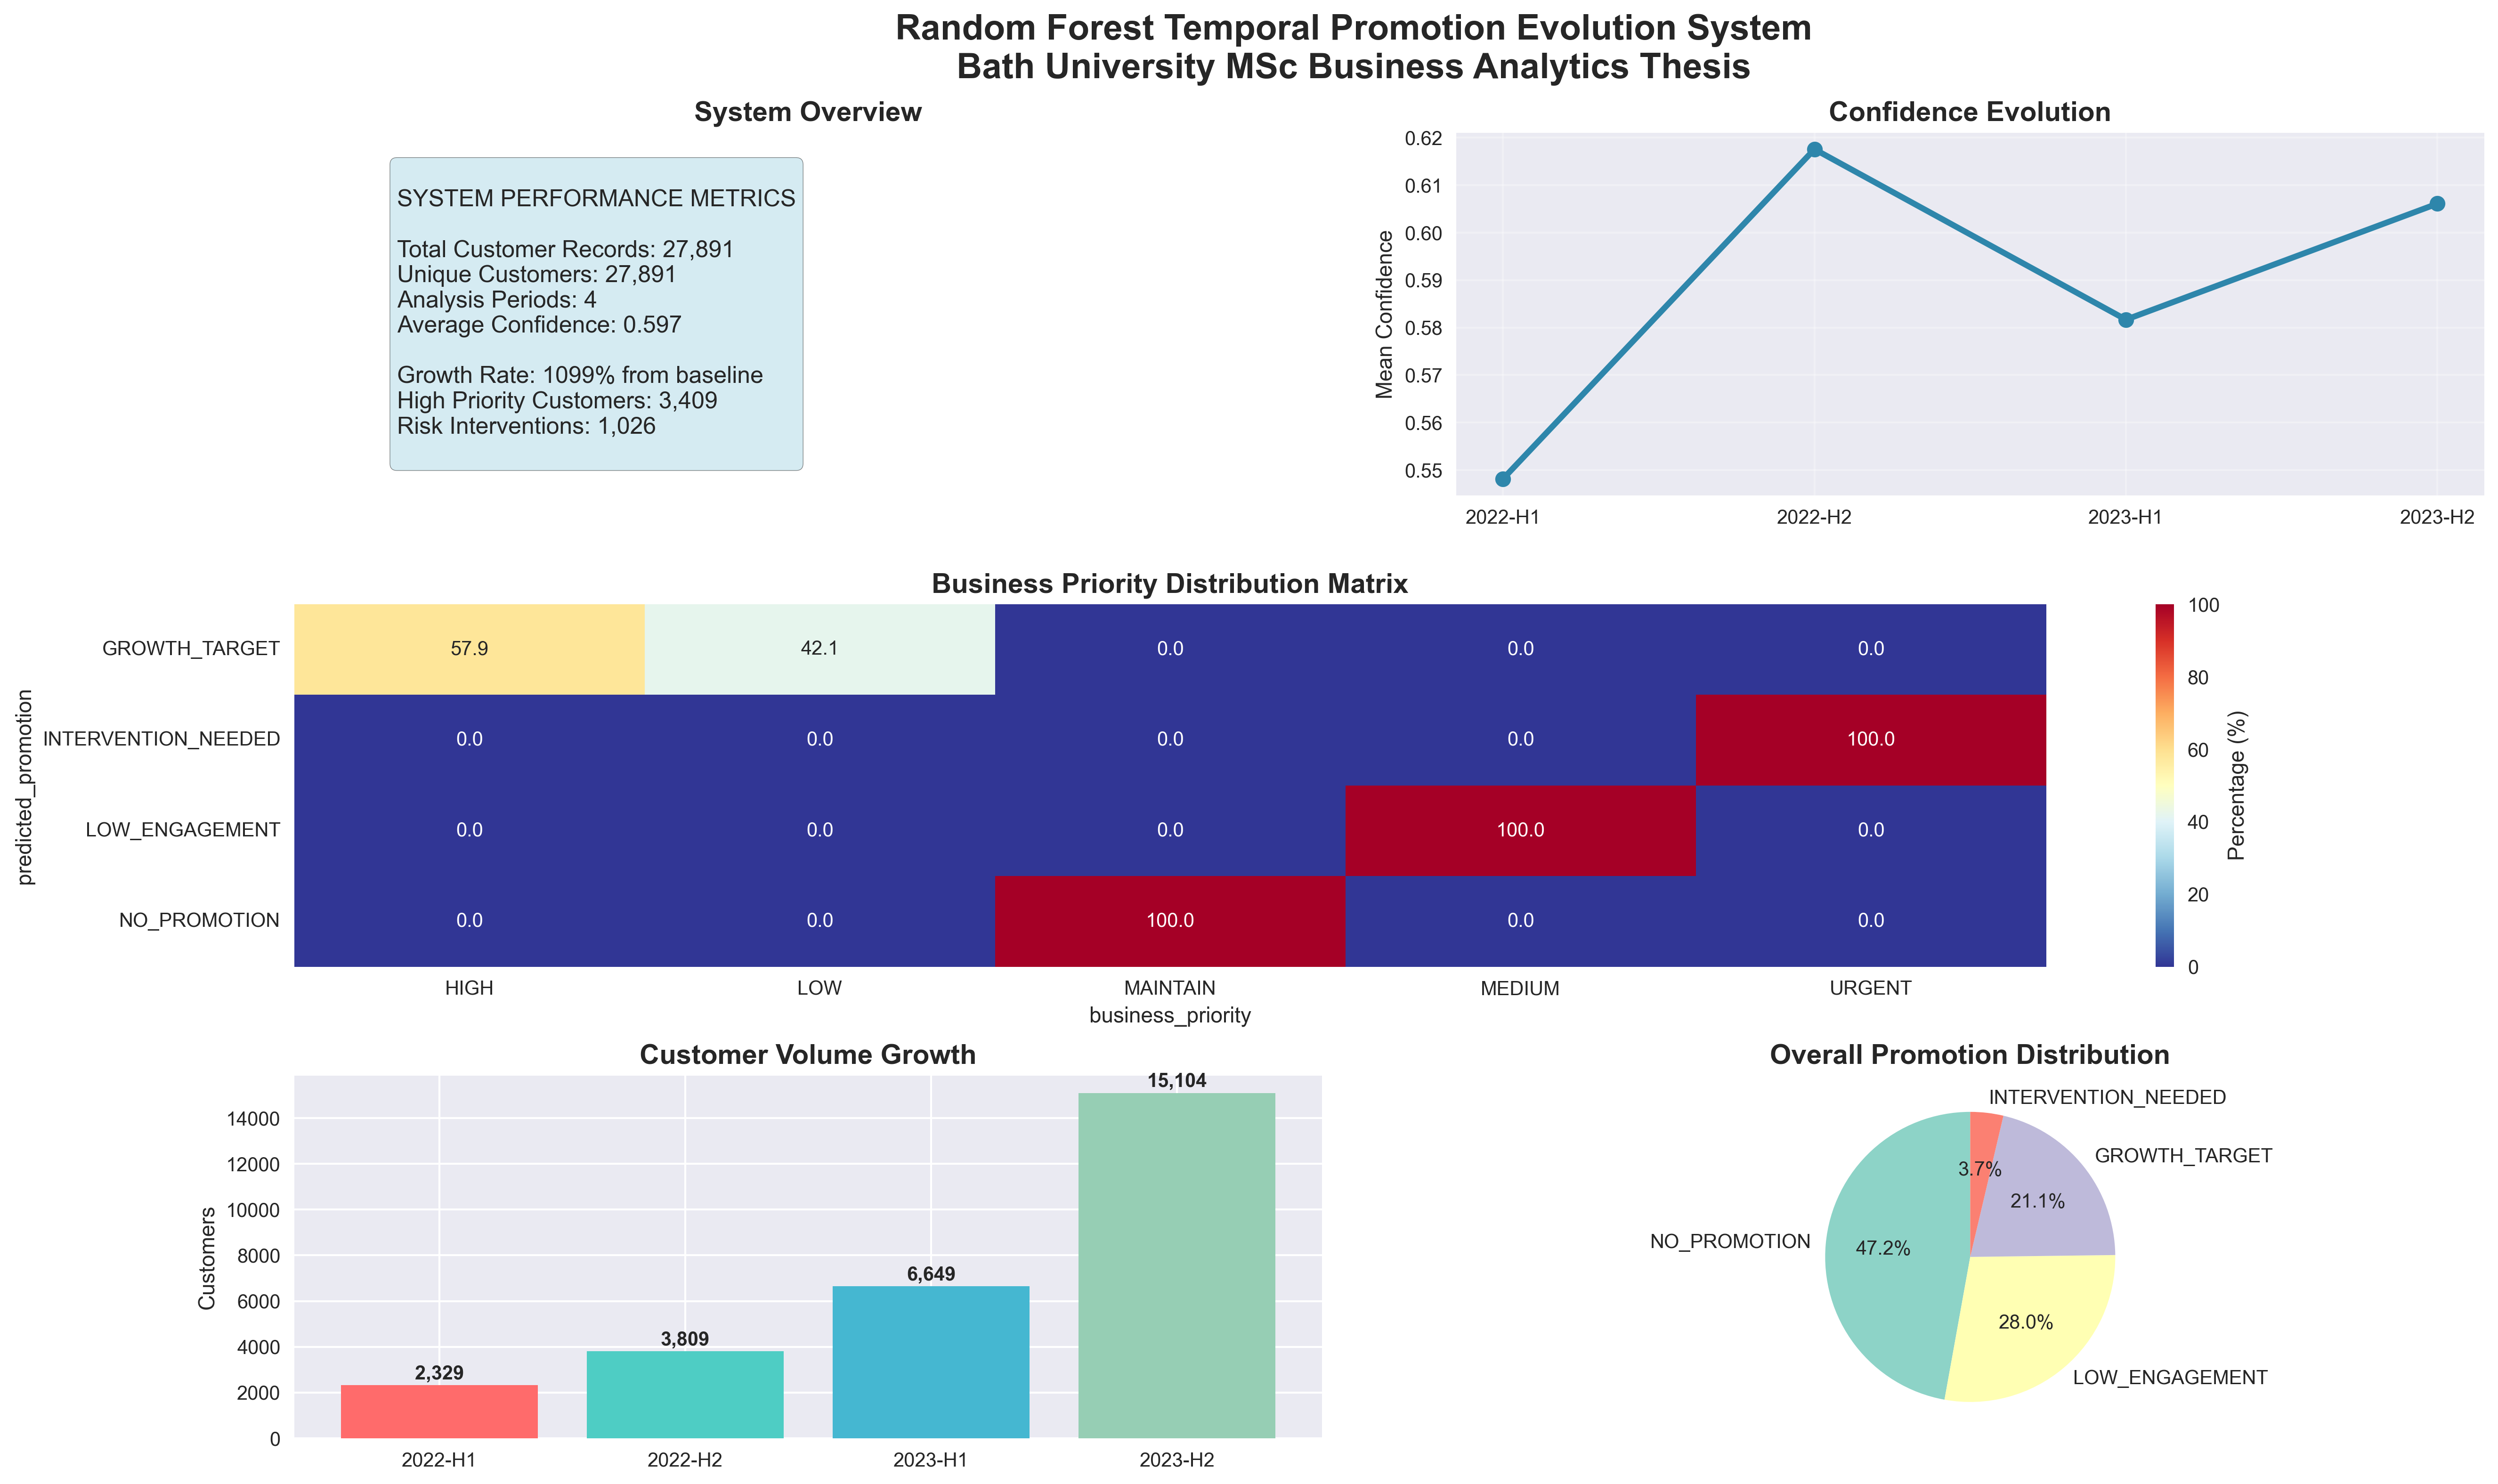
\includegraphics[width=1.03\textwidth]{figures/summary_dashboard.png}
\caption{Unified Dashboard View: Model Statistics, Predictions, and Evolution Indicators (2022--2023)}
\label{fig:unified-summary-dashboard}
\end{figure}

This dashboard serves as a visual summary of the analytical components detailed in Sections~\ref{tab:behavioural_stats_by_period} through \ref{fig:model-confidence}, providing a comprehensive summary of the casino's developing promotional plan within the AI-driven framework. Each subplot in the graphic represents a specific evaluation sub-section, enabling traceability between statistical results and their corresponding methodological context.


\subsubsection*{Behavioural Feature Trends Across Time}

Table~\ref{tab:behavioural_stats_by_period} summarises key customer activity metrics across the five evaluation periods to provide behavioural context for the predicted promotions. The factors encompass average bet amount, average losses, engagement volatility, and loss-chasing tendencies.

The average bet amount increased from €1,237.59 in the first half of 2022 to €2,191.60 in the second half of 2023, reflecting a consistent increase in betting activity. The highest volatility score was recorded in the second half of 2023, at 3,764.58, which may indicate chaotic play styles or inconsistent session durations during that time.

Loss-chasing scores reached their highest point in the first half of 2024, at 48.88, suggesting the presence of a high-risk subgroup that resumed activity following a period of inactivity. Average losses, however, decreased significantly during the same period (€395.47), likely attributable to more conservative betting practices despite stated chasing behaviour.

The number of sessions in the last 30 days increased especially in the second half of 2023 (8.12), before decreasing once more in the first half of 2024. This indicates an unexpected increase in engagement, subsequently followed by a decrease in engagement.

These behavioural dynamics clarify the classifier's evolving promotional strategies. Increased volatility and betting activity in the second half of 2023 may have led to a rise in \textit{GROWTH TARGET} recommendations, while the surge in loss-chasing in the first half of 2024 could indicate a strategic transition towards risk monitoring instead of aggressive retention.

\begin{table}[H]
\centering
\caption{Behavioural Feature Averages Across Evaluation Periods}
\label{tab:behavioural_stats_by_period}
\begin{tabular}{lrrrrrr}
\toprule
\textbf{Period} & \textbf{Avg. Bet} & \textbf{Avg. Loss} & \textbf{Volatility} & \textbf{Loss Chasing} & \textbf{Sessions (30d)} & \textbf{Bet Trend} \\
\midrule
2022-H1 & 1237.59 & 1299.20 & 1247.496 & 23.270 & 2.37 & 1.000 \\
2022-H2 & 1354.46 & 1806.07 & 1442.520 & 25.950 & 2.53 & 1.100 \\
2023-H1 & 1663.15 & 1591.24 & 1854.301 & 29.876 & 3.68 & 1.200 \\
2023-H2 & 2191.60 & 1375.34 & 3764.582 & 23.478 & 8.12 & 1.300 \\
2024-H1 & 2161.32 & 395.47  & 2203.161 & 48.880 & 1.71 & 1.100 \\
\bottomrule
\end{tabular}
\end{table}

\subsection{Promotion Distribution by Period}
\label{sec:promotion_distribution}

Number of Term Customs: To evaluate the model's promotional response logic, predictions were evaluated across four assessment periods. Figure~\ref{fig:promotion-distribution} illustrates the proportional allocation of customers designated to each promotional category: \texttt{GROWTH\_TARGET}, \texttt{INTERVENTION\_NEEDED}, \texttt{LOW\_ENGAGEMENT}, and \texttt{NO\_PROMOTION}.

\begin{figure}[H]
\centering
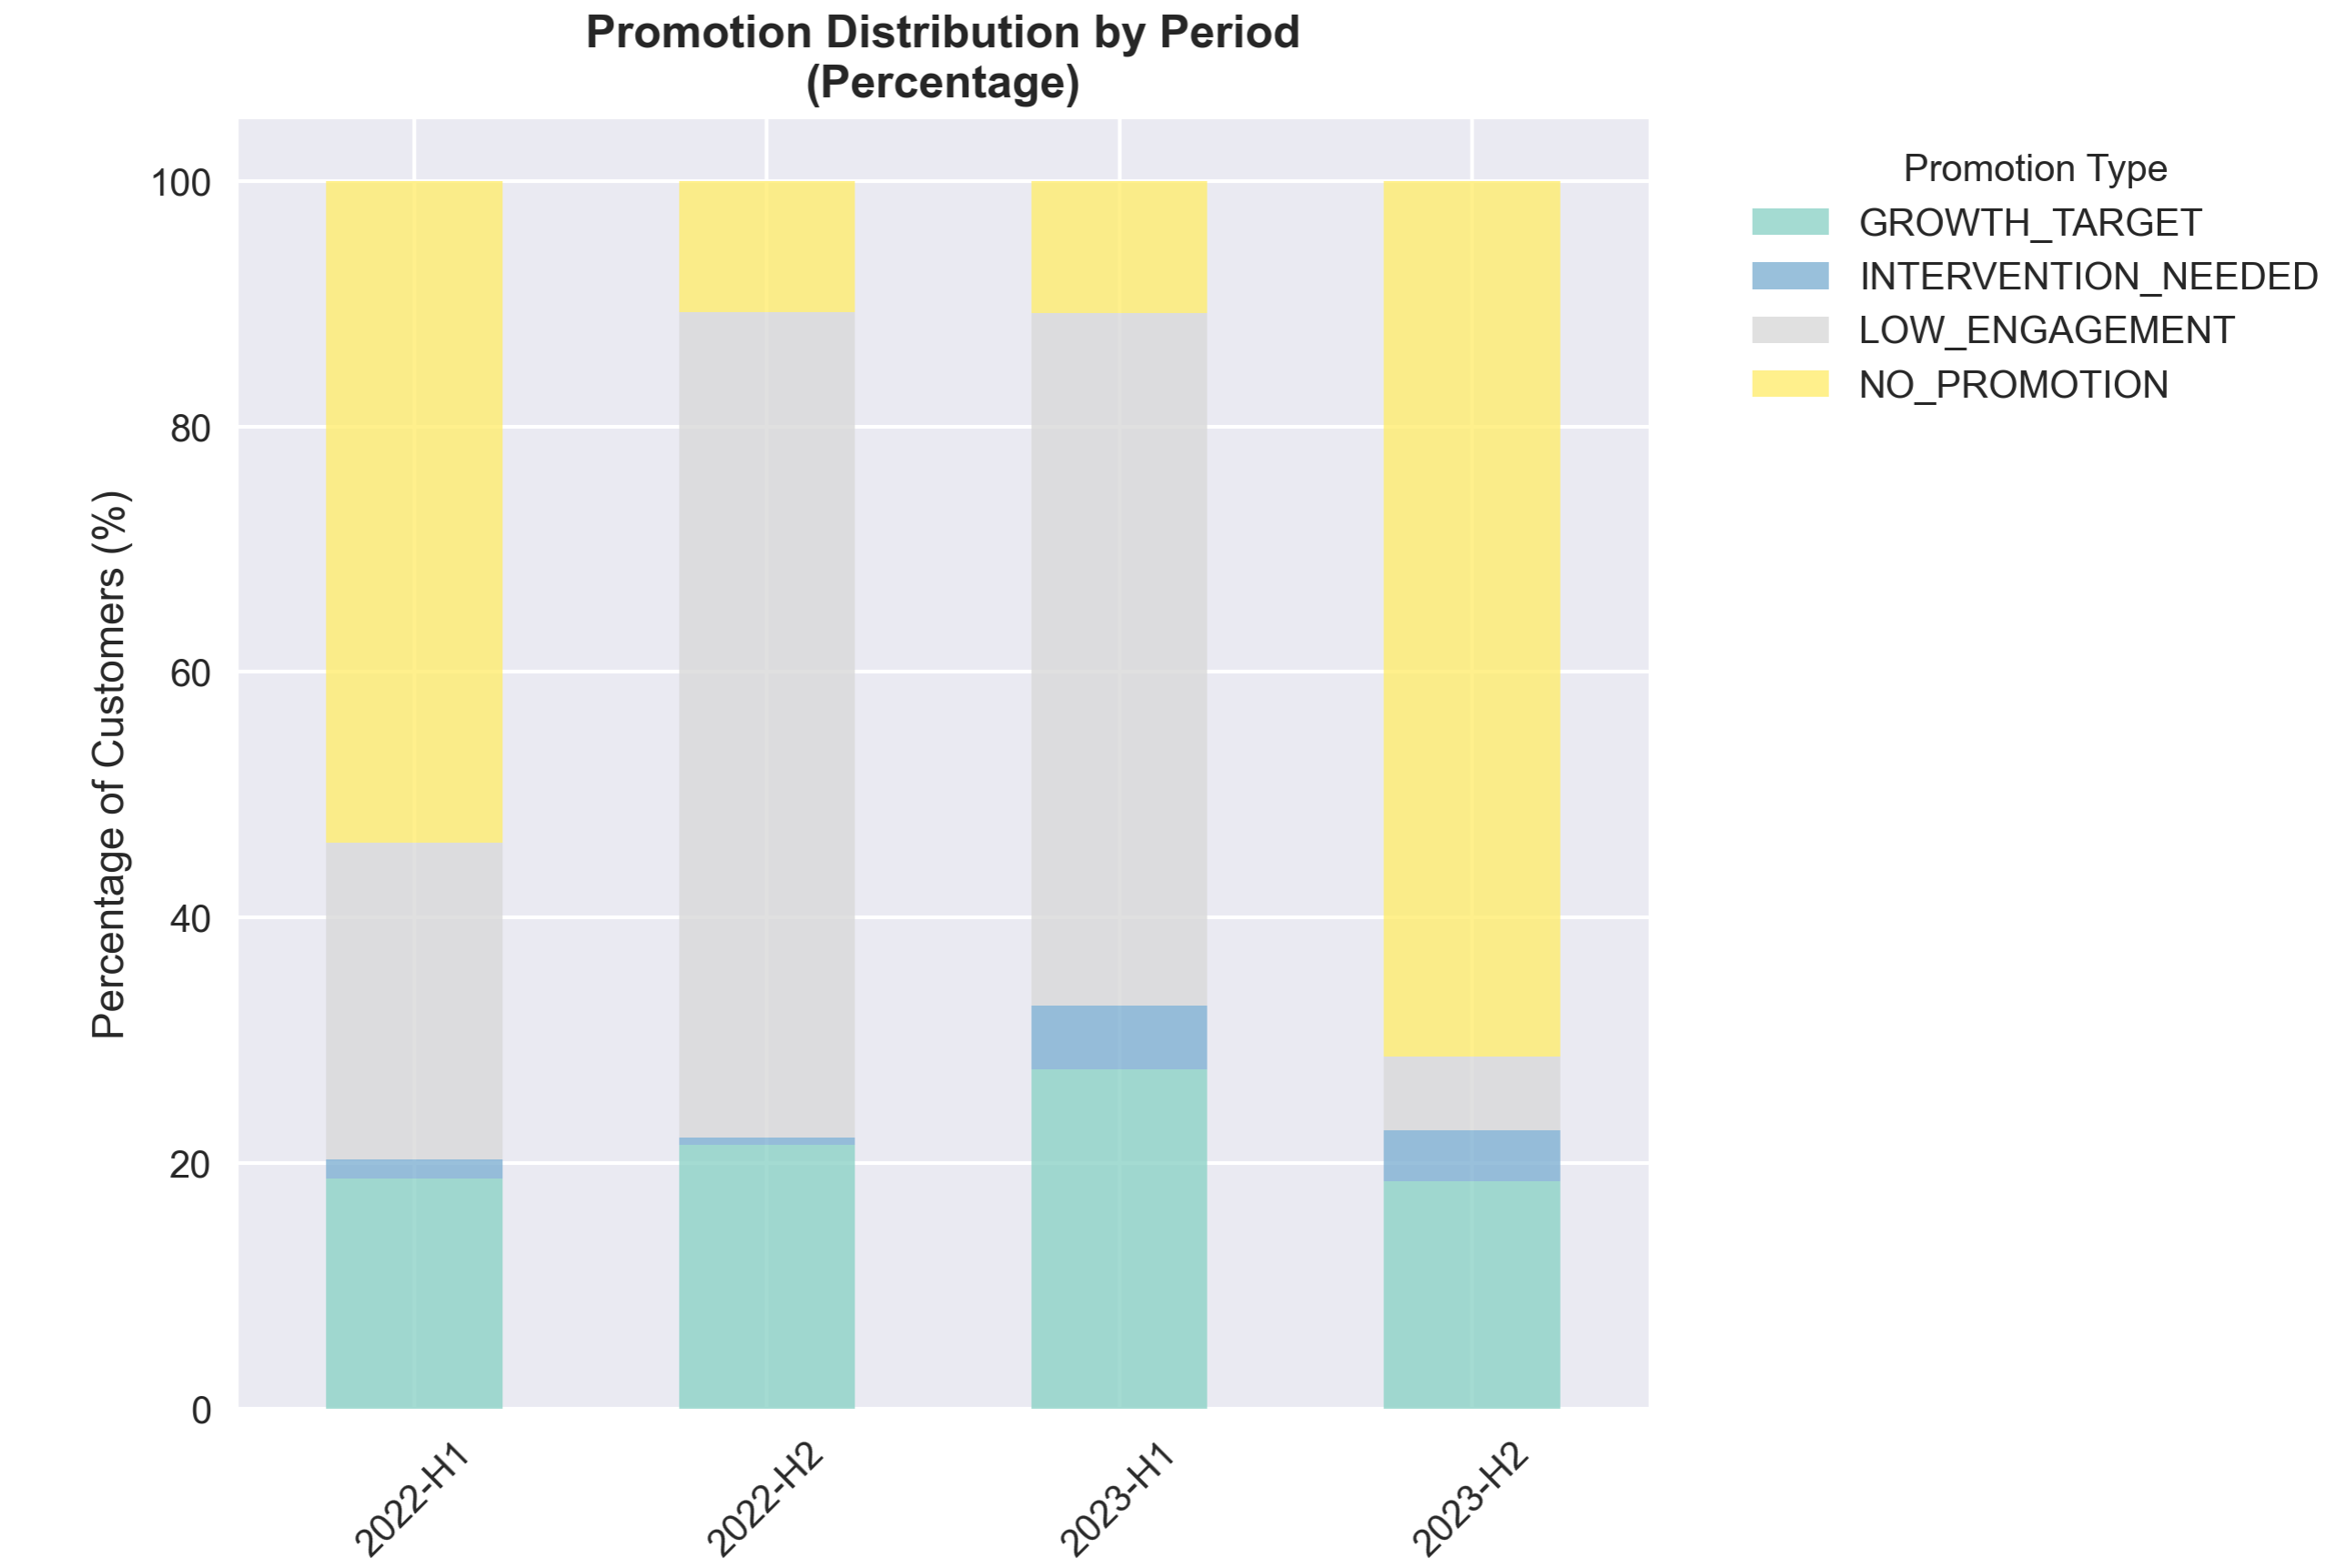
\includegraphics[width=0.85\textwidth]{figures/promotion_distribution_by_period.png}
\caption{Promotion distribution across analysis periods, grouped by predicted promotional categories.}
\label{fig:promotion-distribution}
\end{figure}

The graphic illustrates the variation in the distribution of expected promotional categories over the four assessed periods. Significantly, the percentage of clients identified as \texttt{GROWTH\_TARGET} and \texttt{INTERVENTION\_NEEDED} increased steadily over time. In 2022-H1, the majority of players were classified as \texttt{NO\_PROMOTION}, indicating either low activity or insufficient behavioural signals. By 2023-H2, however, a clear shift is observed: the share of customers predicted as eligible for targeted promotional actions rose substantially, especially in the \texttt{GROWTH\_TARGET} category.

This change shows that both the accuracy of the behavioural features is getting better and the classifier is becoming more sure that it can target specific segments.  The system could adapt to a bigger set of data and find players with more ability to engage or higher behavioural risk more accurately.

\subsection{Business Priority Alignment}

The AI system's primary goal was to coordinate the anticipated types of promotions with the company's long-term objectives. Based on the standards set by the casino management, every customer was given a behavioural segment and then linked to a business priority label, such as \texttt{HIGH}, \texttt{MEDIUM}, \texttt{MAINTAIN}, \texttt{LOW}, or \texttt{URGENT}.

Figure~\ref{fig:priority-matrix} illustrates the alignment matrix between promotional response categories and strategic priorities. For instance, \texttt{GROWTH\_TARGET} customers were mostly aligned with \texttt{HIGH} and \texttt{LOW} priorities, while \texttt{INTERVENTION\_NEEDED} cases were concentrated under the \texttt{URGENT} tier. This illustrates the model's capacity to generate actionable results by aligning machine-generated categories with strategically defined domain layers.

This alignment is helpful for CRM operators since it clearly confirms that the promotional activity is matched with the consumer categories that need attention. This matrix is a useful qualitative tool for assessing the model's interpretability and practical applicability; it was created using results from the Random Forest model that was tested from 2022 to 2023.

\begin{figure}[H]
\centering
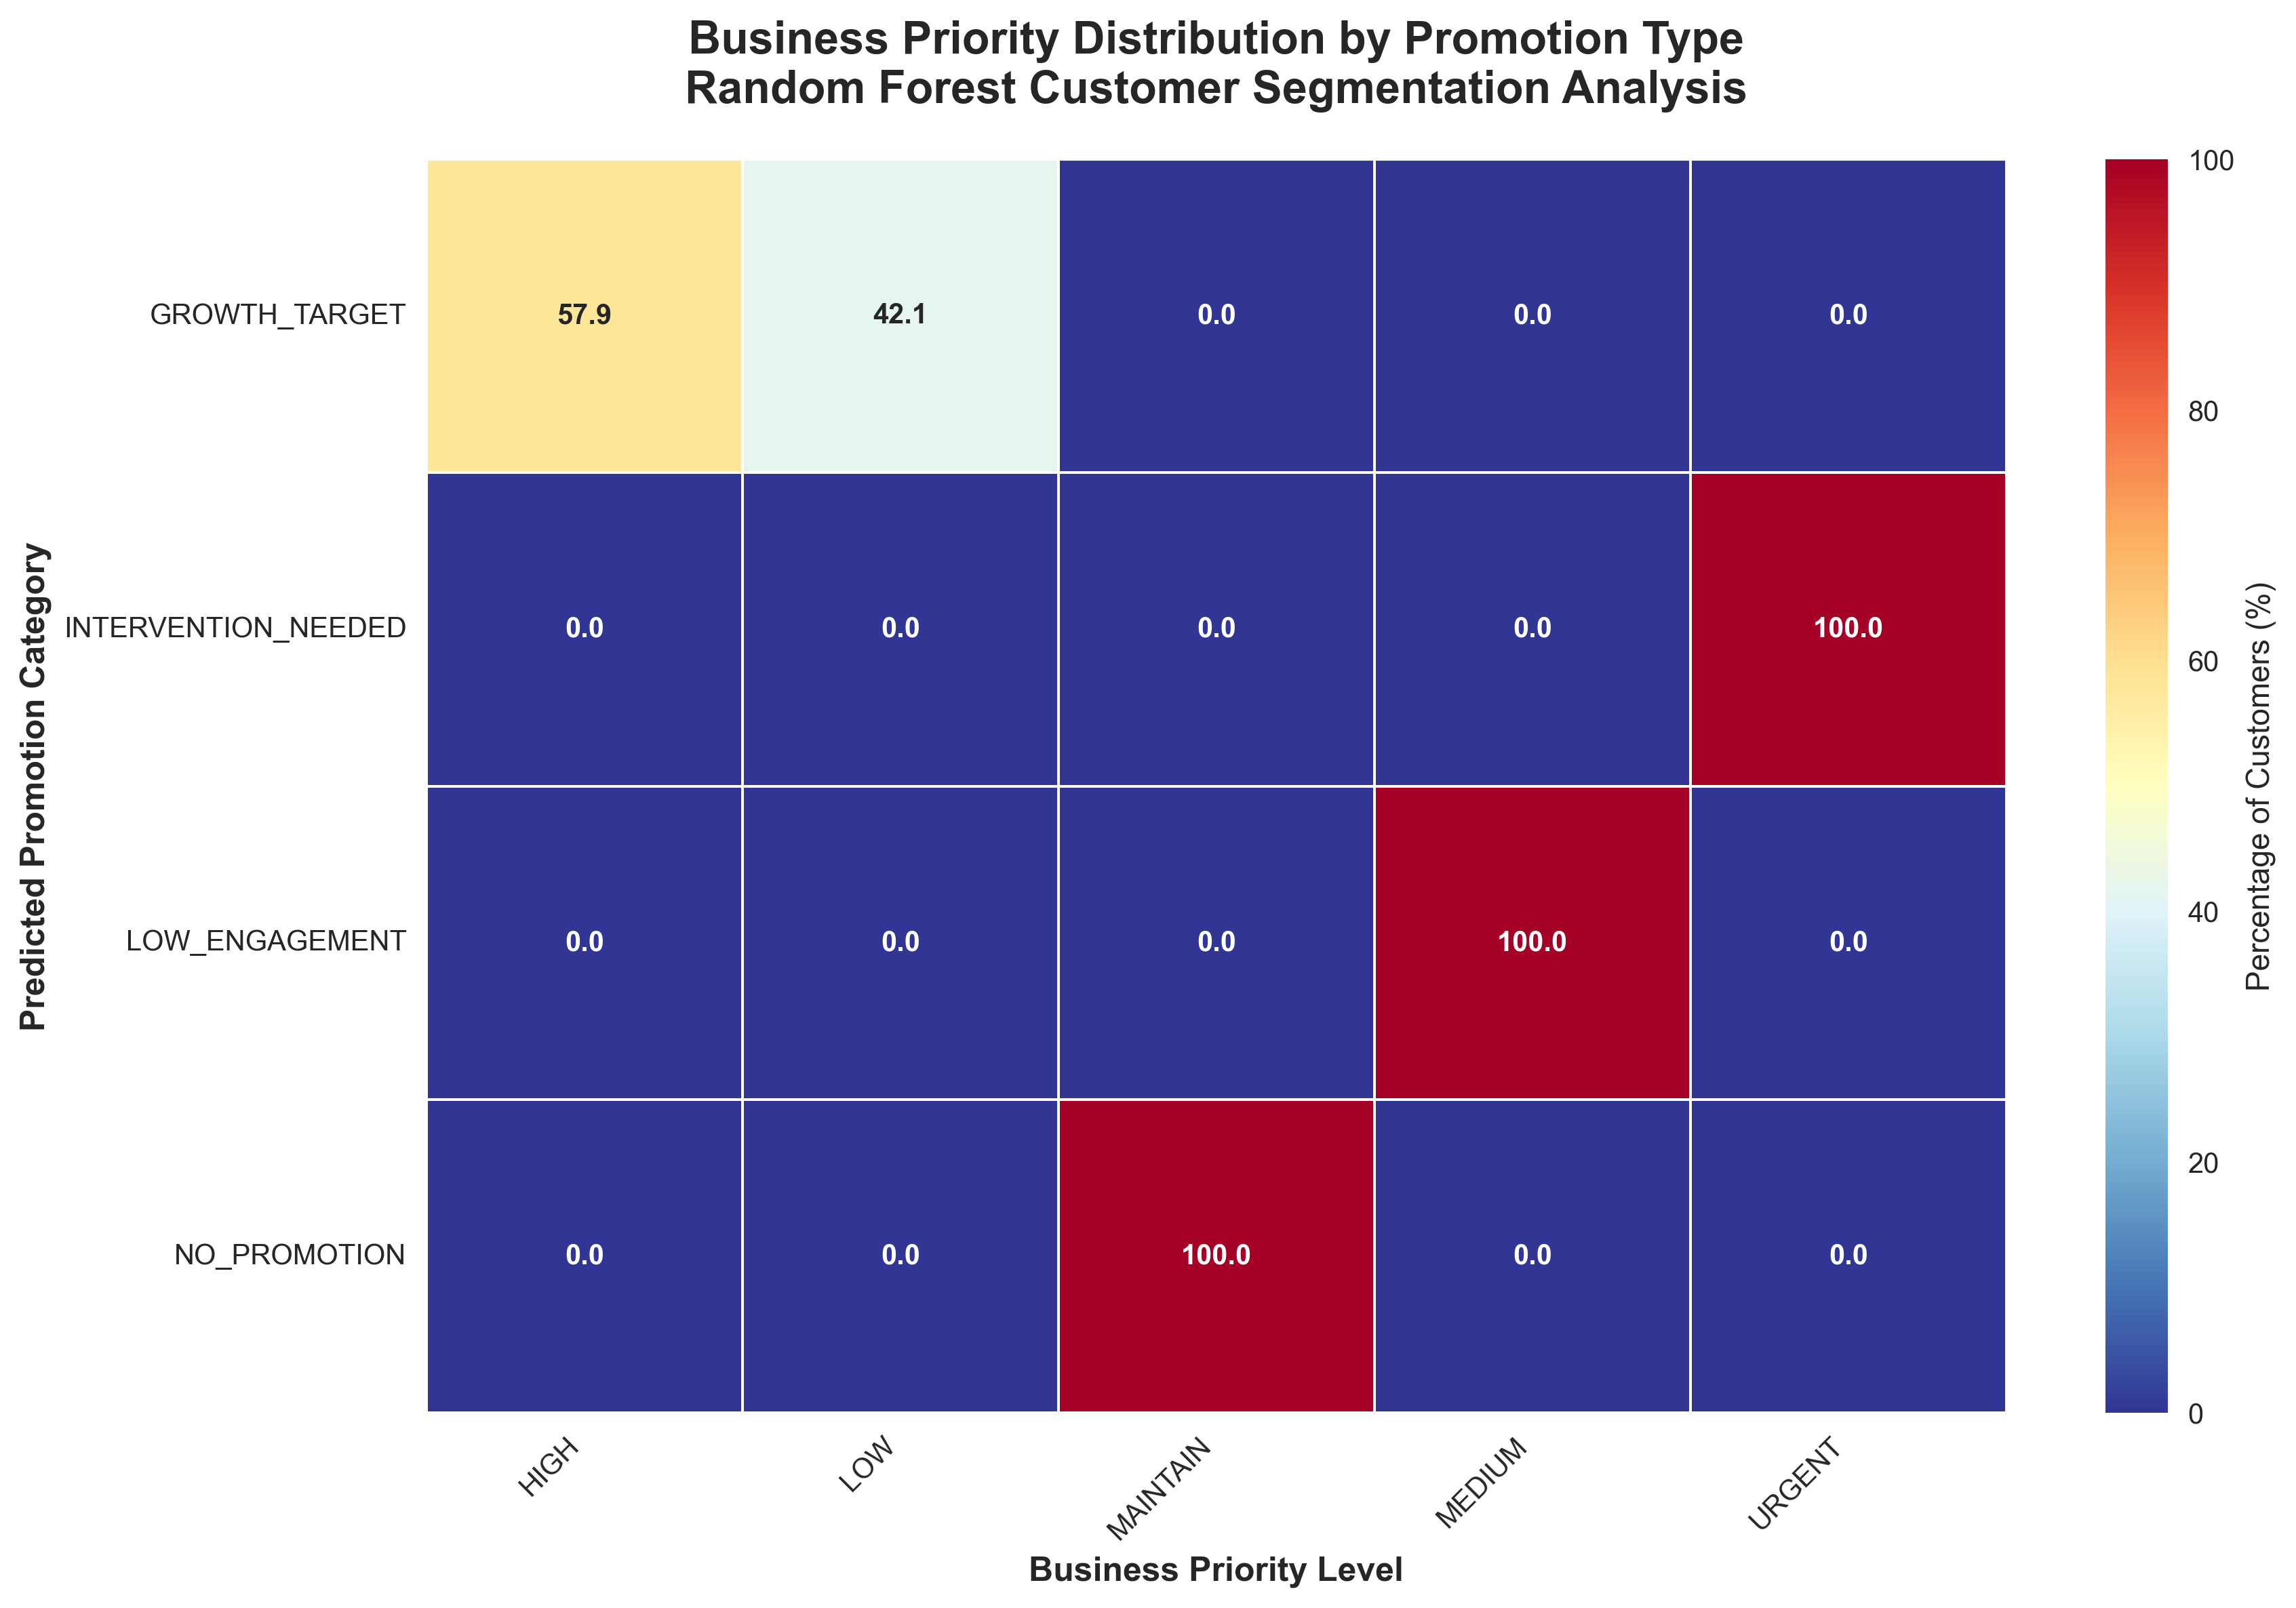
\includegraphics[width=0.95\textwidth]{figures/priority_distribution_matrix.png}
\caption{Business Priority Distribution Matrix by Predicted Promotion Category}
\label{fig:priority-matrix}
\end{figure}

\section*{Model Confidence Overview}

In order to determine how stable and reliable the Random Forest classifier was, we examined prediction confidence over all evaluation periods.  A customer's confidence score is a measure of how sure they are in a decision since it reflects the probability that the model has given to each customer's expected promotional category.

As shown in Figure~\ref{fig:model-confidence}, mean confidence levels remained relatively stable across periods, ranging from 0.548 in 2022-H1 to 0.618 in 2022-H2, before returning to 0.606 by 2023-H2. According to these numbers, the model was able to keep its forecasts consistently certain even as the number of customers and the complexity of their behaviours increased.

The figure provides a detailed breakdown: the left-hand line chart illustrates the evolution of average confidence, with shaded bands representing ±1 standard deviation to indicate variance. The boxplot on the right visualises confidence score distributions across customers, showing tight clustering around the median—particularly in later periods—implying improved model calibration and lower variance.

In general, the system showed strong trust calibration throughout deployment. This level of consistency is important for production-level adoption because it lets CRM teams run bigger campaigns while still trusting that the AI-driven recommendations are correct.


\begin{figure}[H]
\centering
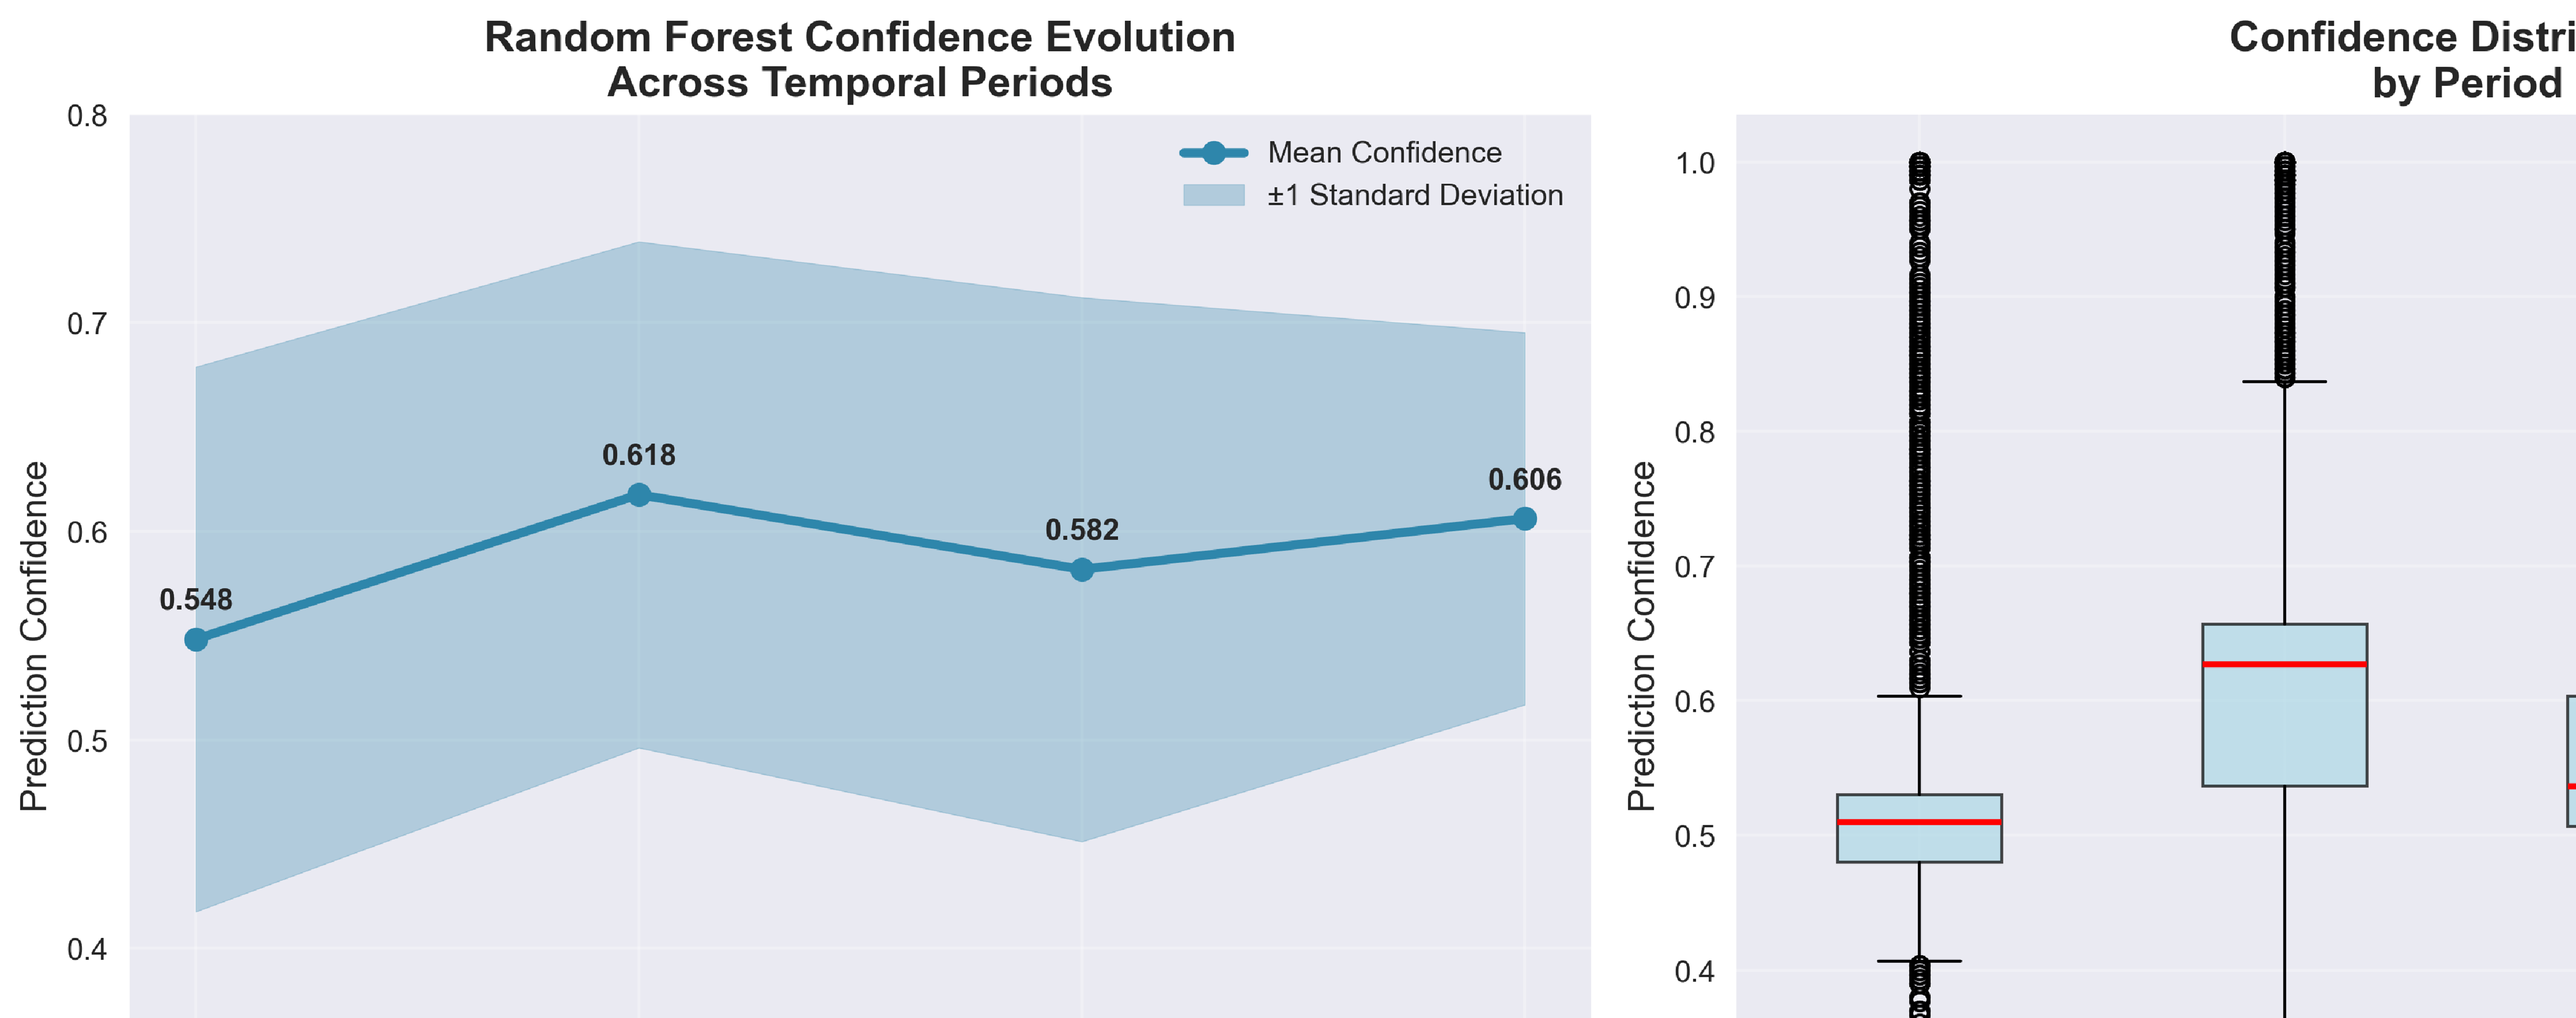
\includegraphics[width=0.95\textwidth]{figures/model_confidence.png}
\caption{Business Priority Distribution Matrix by Predicted Promotion Category}
\label{fig:model-confidence}
\end{figure}

%-------------------------------------------------------------------------------

\section{Segment-Based Promotion Results} 
\label{sec:segment_promotion_results}

To evaluate the model’s strategic alignment with customer typologies, this section presents the predicted promotional distributions across behavioural segments: \textit{Casual Players}, \textit{Regular Players}, and \textit{High Rollers}. These segments were identified via unsupervised K-Means clustering and retained consistently across all four evaluation periods.

This test is intended to see whether the AI system uses different promotional reasoning based on segment characteristics, like how active a segment is, how often they lose interest, or how often they change their engagement. Businesses expect High Rollers to get more direct promotional messages, while Casual players may be able to get lighter, more retention-focused deals.

Figure~\ref{fig:segment_promo_dist} illustrates the distribution of predicted promotion types across customer segments, allowing us to evaluate whether the Random Forest classifier has internalised meaningful behavioural typologies during training.


\section{Temporal Promotion Evolution}
\label{sec:temporal_promo_evolution}

This section examines the evolution of the AI-driven promotional strategy across four analysis periods: 2022-H1, 2022-H2, 2023-H1, and 2023-H2. The goal is to assess whether the Random Forest classifier exhibited temporal adaptability in terms of promotion targeting and model confidence.

\subsection*{Promotion Distribution Across Periods}
Figure~\ref{fig:promo_by_period} shows the percentage distribution of predicted promotion types across the four evaluation periods. A clear trend is observed: the proportion of customers receiving NO\_PROMOTION recommendations decreased over time, while GROWTH\_TARGET and INTERVENTION\_NEEDED recommendations increased—suggesting improved segment engagement and model assertiveness.

\begin{figure}[H]
    \centering
    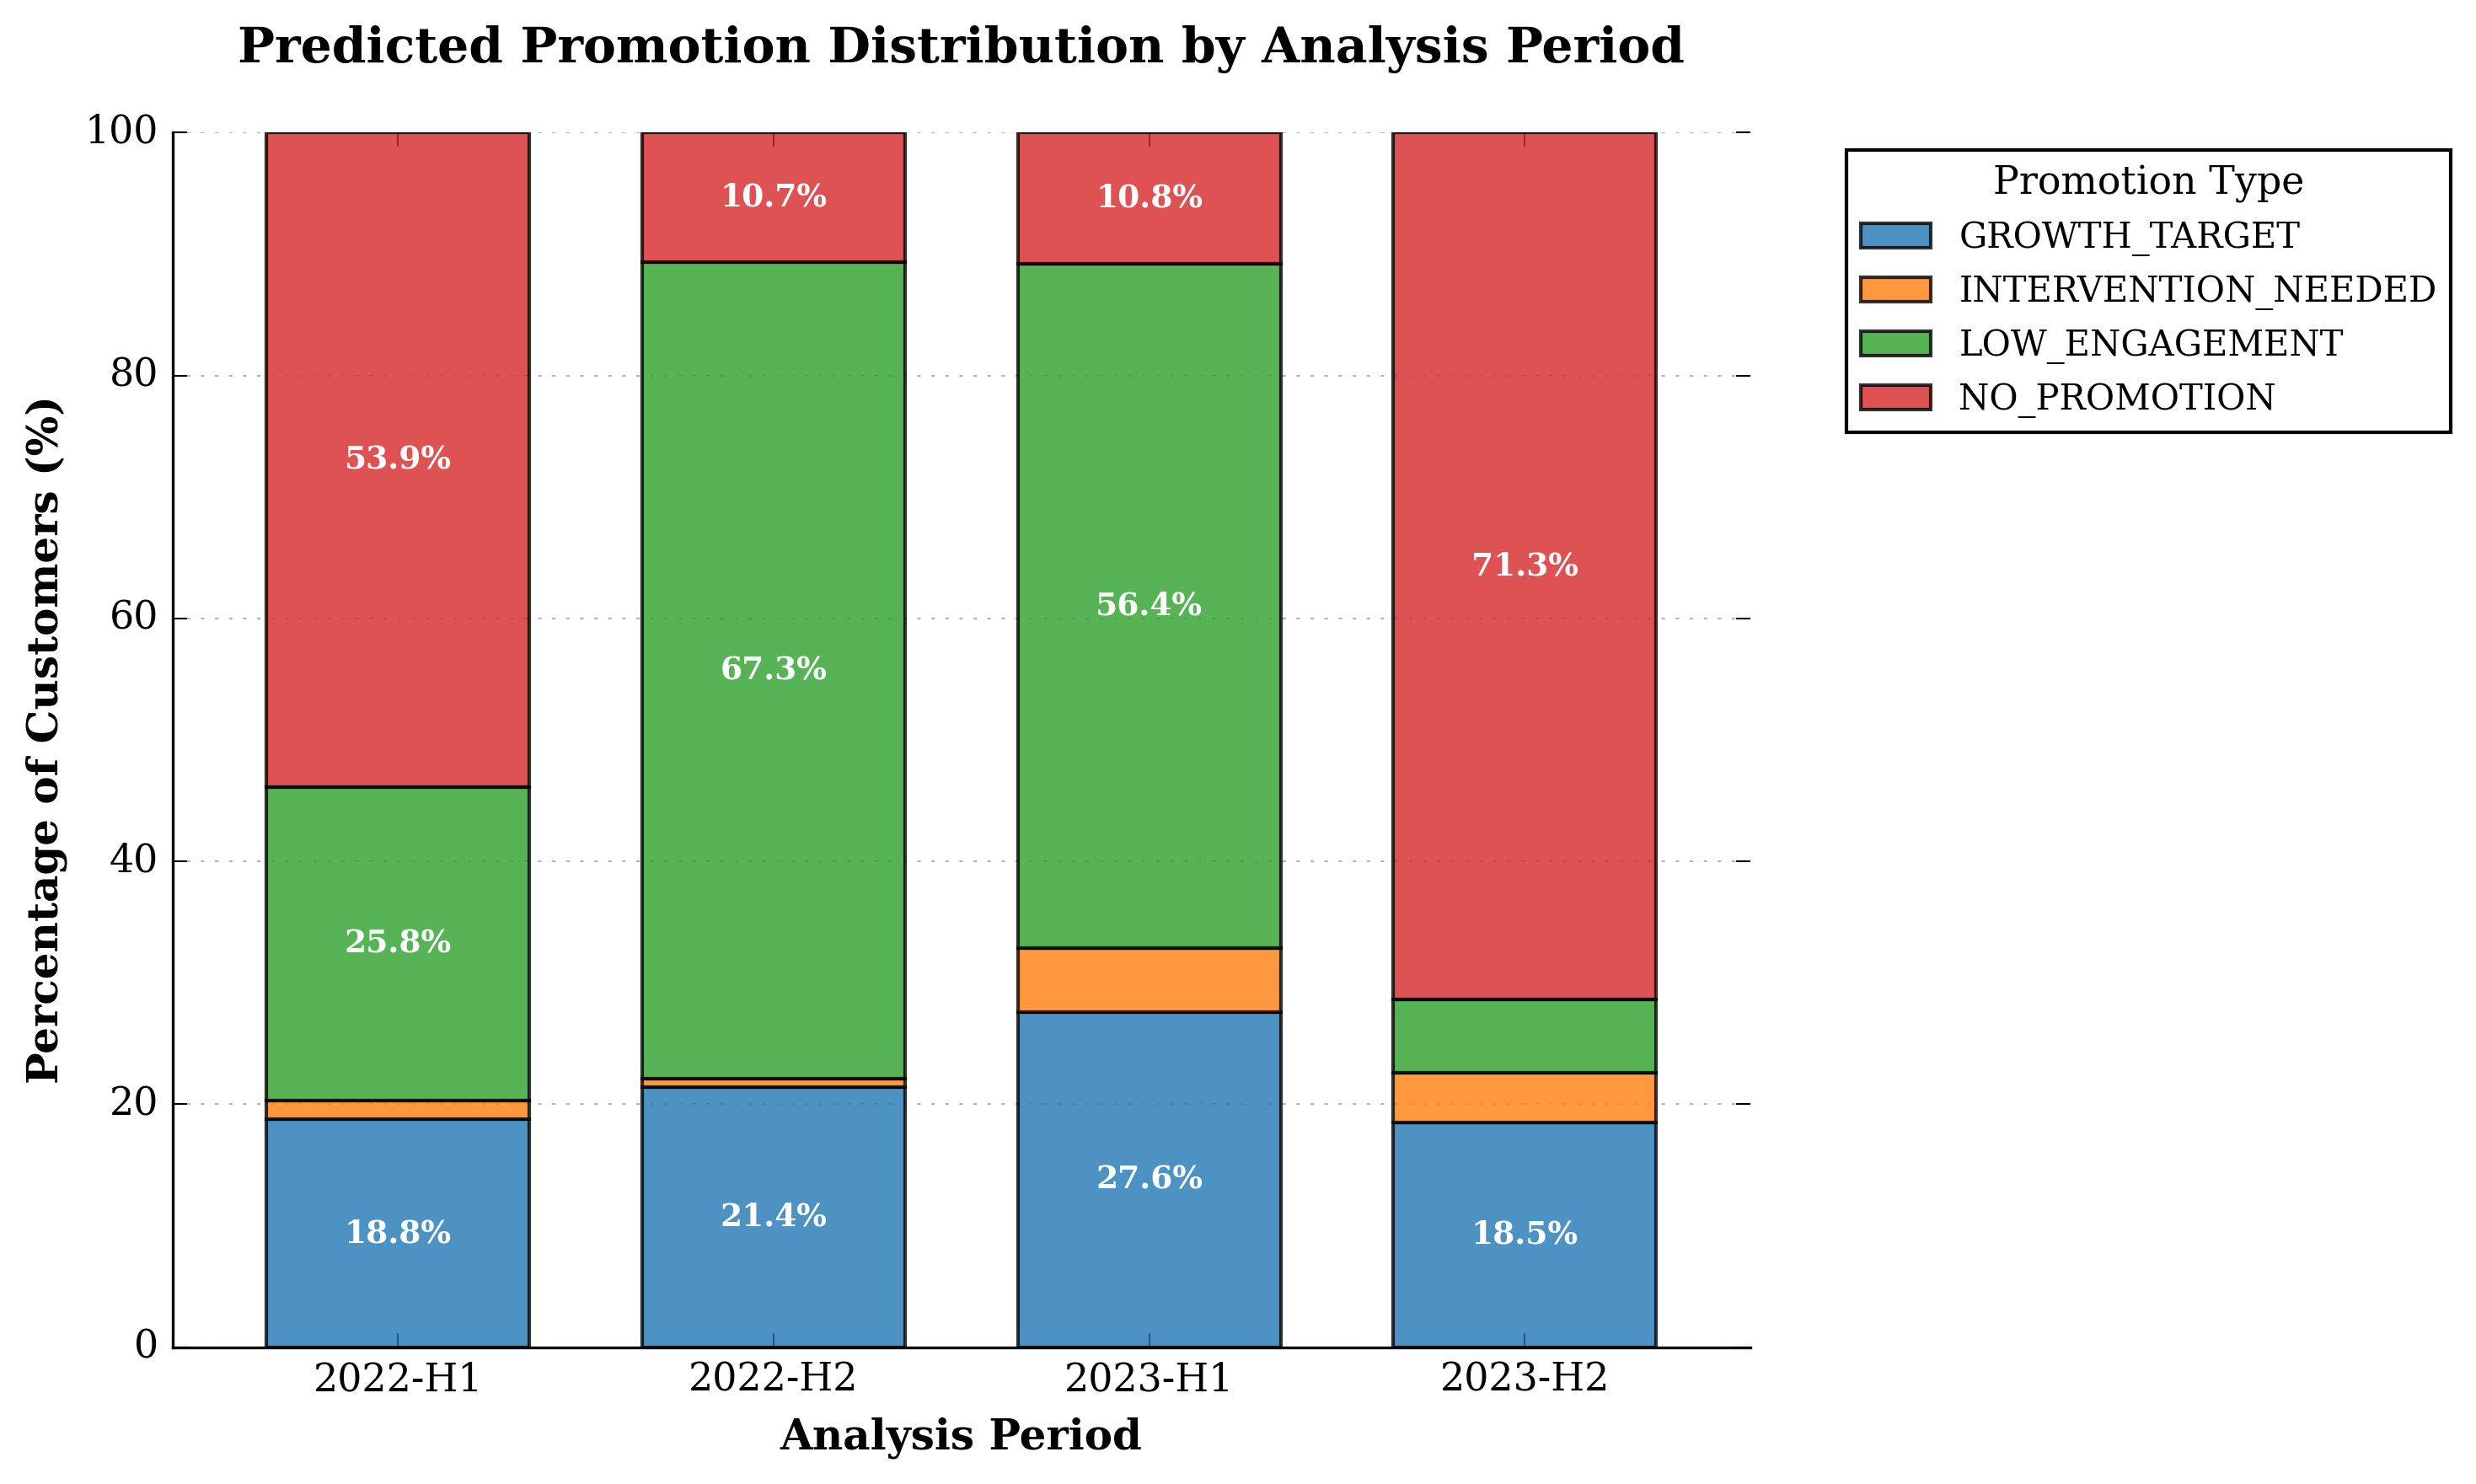
\includegraphics[width=0.8\textwidth]{figures/promotion_by_period.png}
    \caption{Predicted Promotion Distribution by Period}
    \label{fig:promo_by_period}
\end{figure}

\subsection*{Model Confidence Evolution}
The AI system’s average confidence scores per period are depicted in Figure~\ref{fig:confidence_line}. While slight fluctuations occurred, overall model confidence improved from 0.548 in 2022-H1 to 0.606 in 2023-H2. This indicates better feature-pattern matching and classifier calibration over time.

\begin{figure}[H]
    \centering
    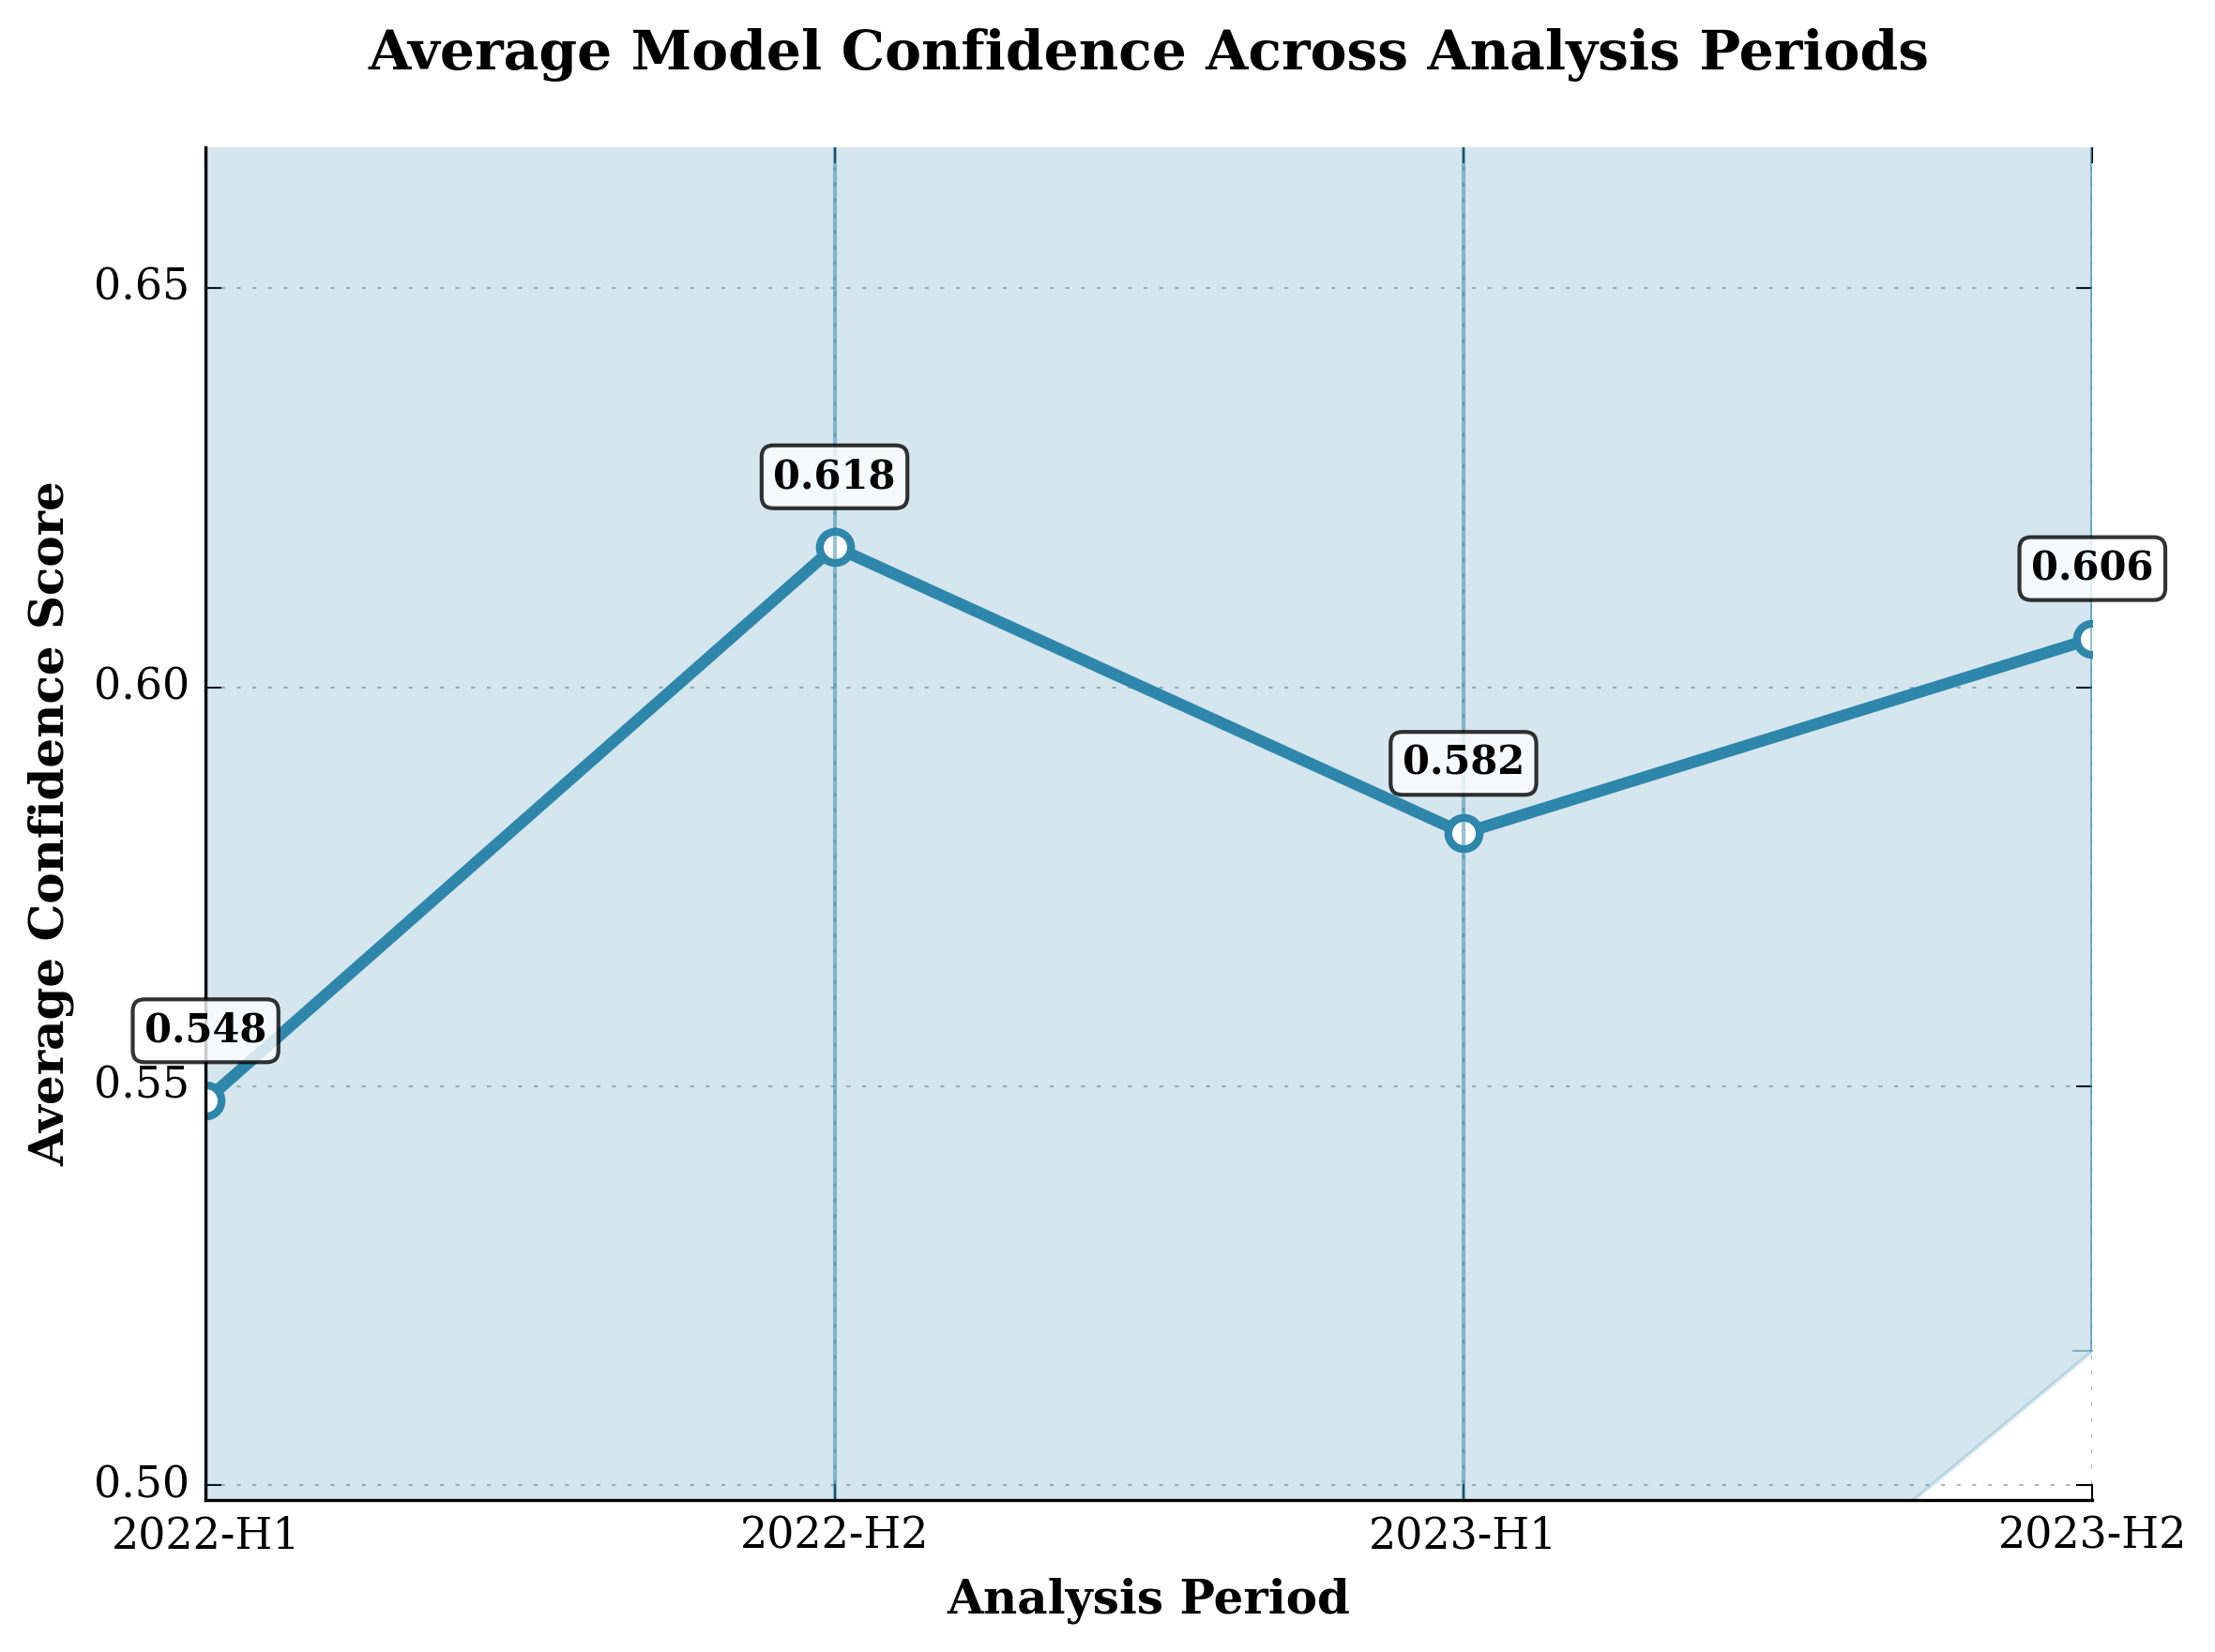
\includegraphics[width=0.7\textwidth]{figures/confidence_lineplot.png}
    \caption{Average Model Confidence Across Periods}
    \label{fig:confidence_line}
\end{figure}

\subsection*{Confidence Distribution and Variance}
As shown in Figure~\ref{fig:confidence_boxplot}, the distribution of confidence scores became tighter in later periods, with fewer outliers and reduced variance. This reinforces the reliability of model predictions as training data increased and behavioural patterns stabilized.

\begin{figure}[H]
    \centering
    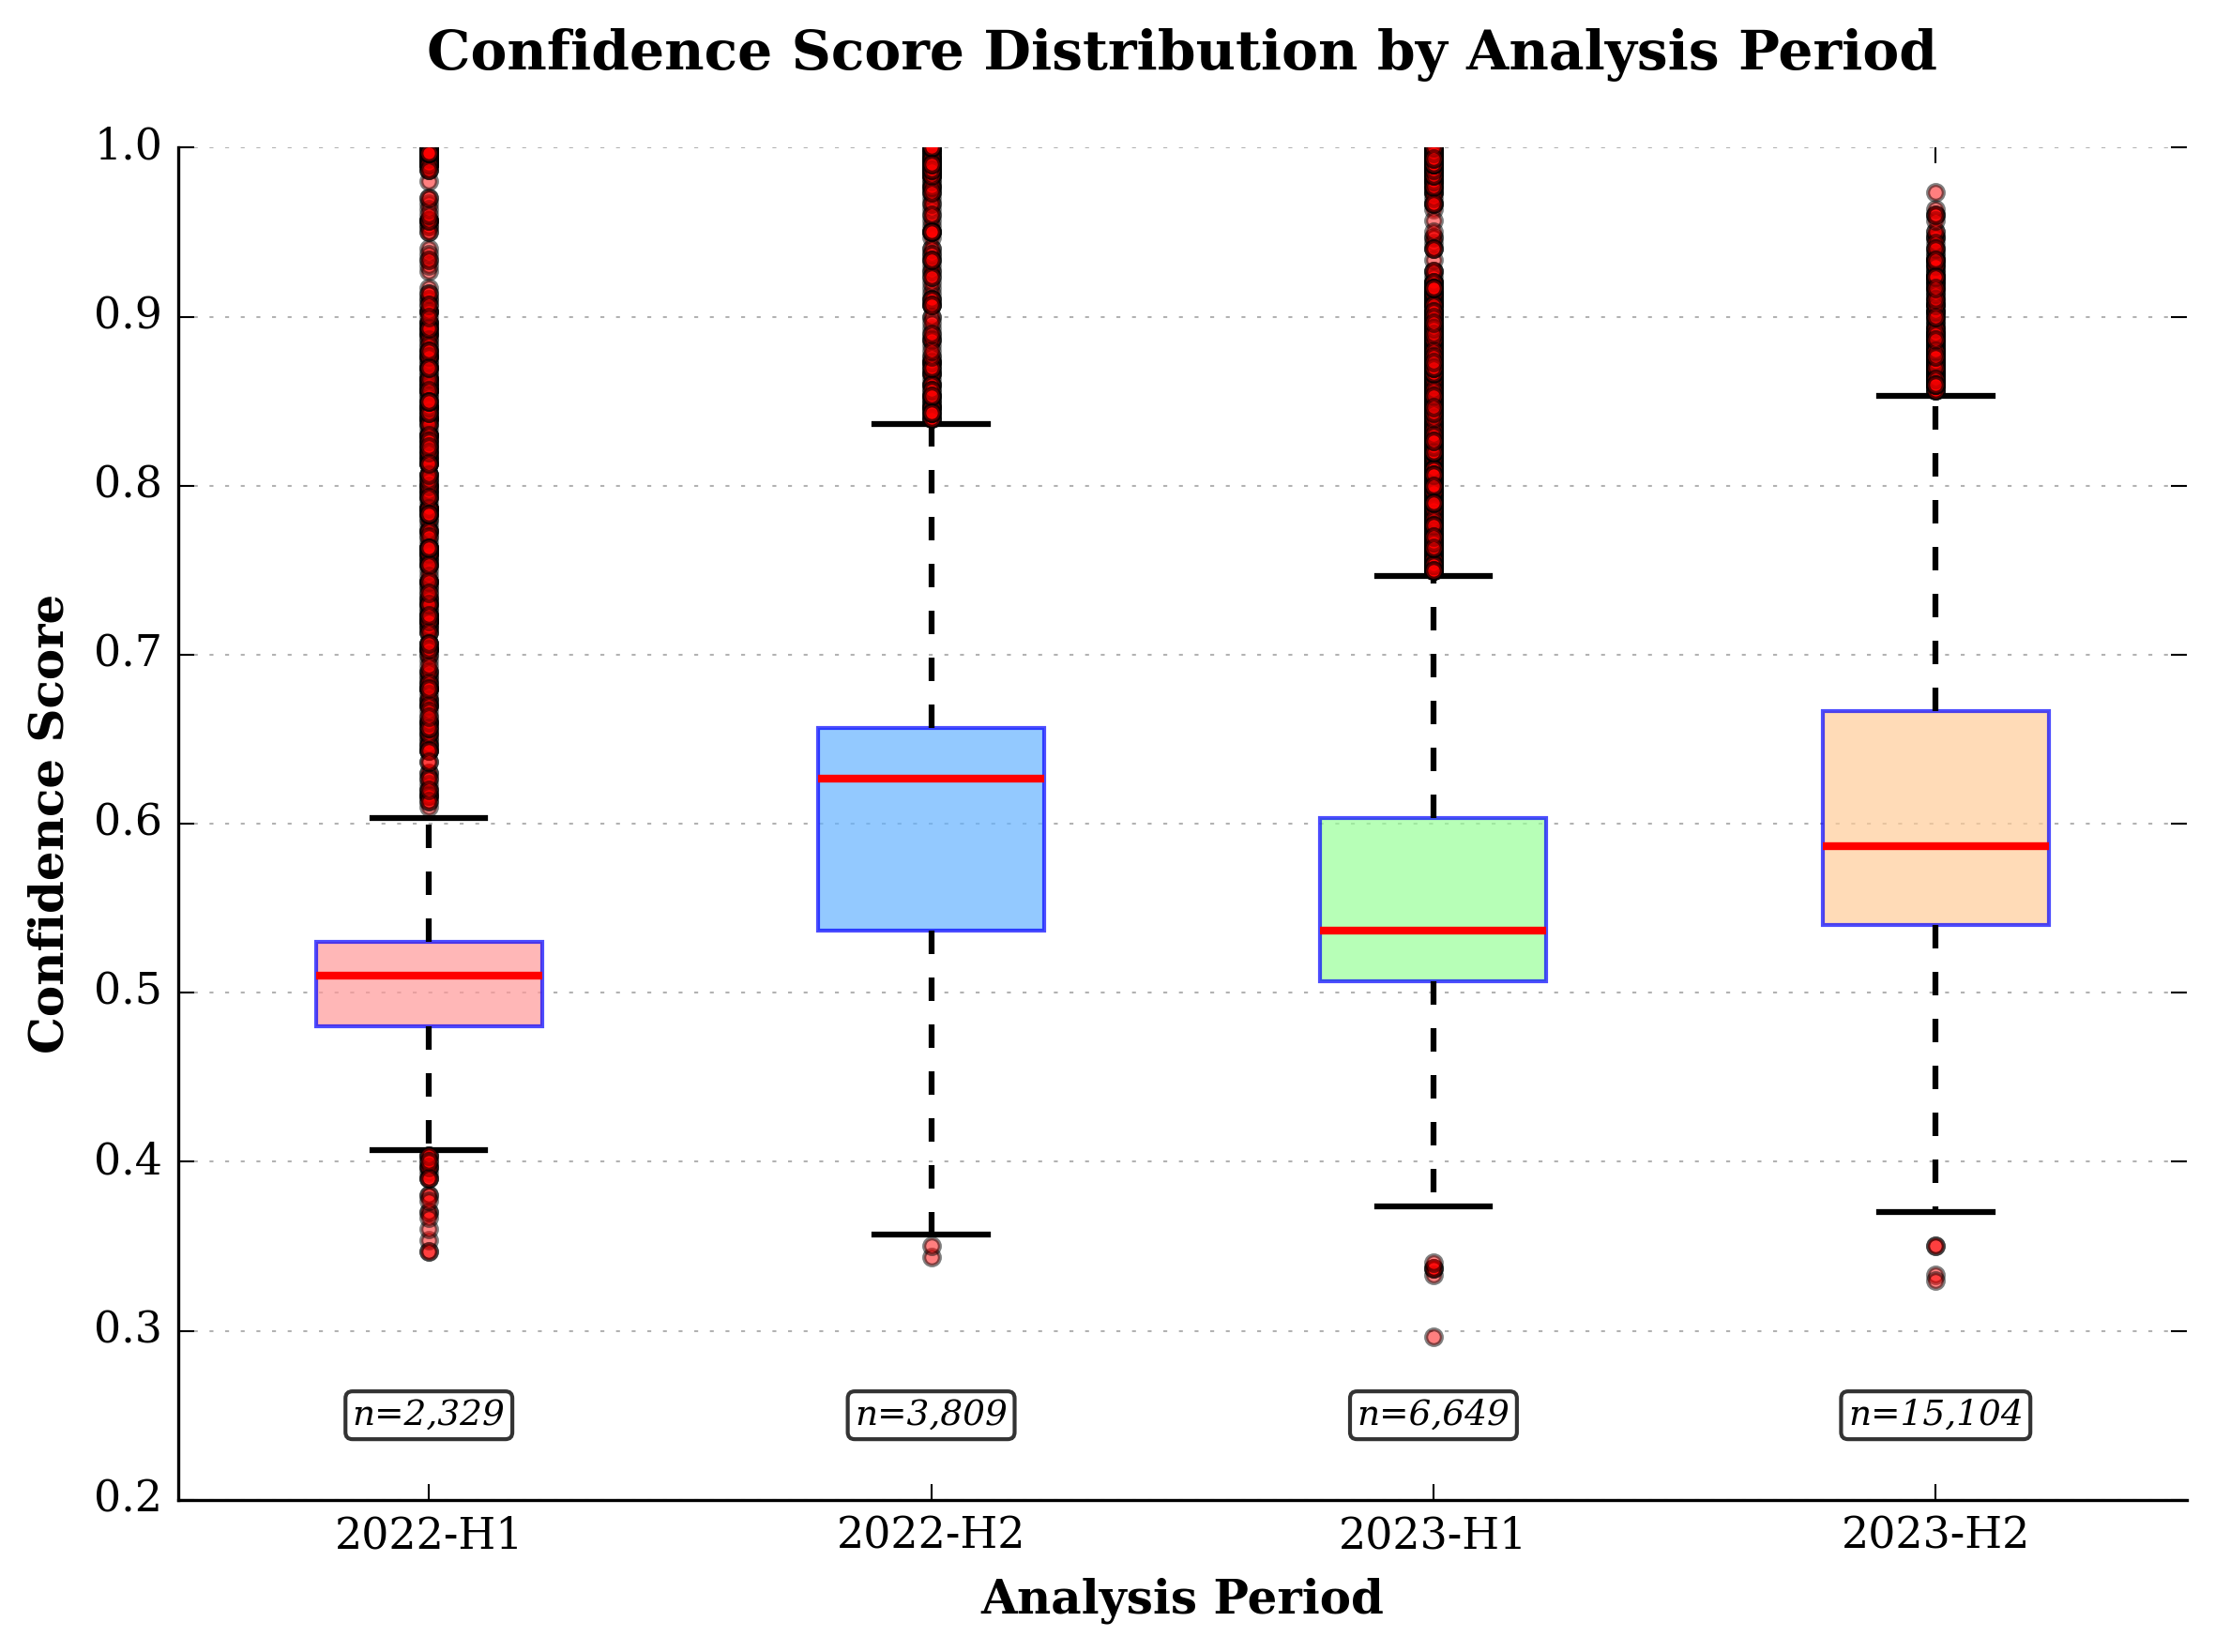
\includegraphics[width=0.7\textwidth]{figures/confidence_boxplot.png}
    \caption{Confidence Score Distribution by Period}
    \label{fig:confidence_boxplot}
\end{figure}


The left heatmap shows intra-segment distributions and shows that most \textit{Casual Players} (62.9\%) did not receive a promotional suggestion, which is in line with how little they usually interact with the site. \textit{High Rollers}, on the other hand, were mostly labelled as \textit{Low Engagement} label (68.9\%). This was probably because their play changed a lot or they didn't play high-stakes games very often, which made CRM teams think about soft interventions instead of bonus-based reactivation.

The spread of \textit{Regular Players} was the most even, with 25.7\% predicted as \textit{GROWTH TARGET} and 18.5\% predicted as \textit{Low Engagement}. This means that the model can pick up on regular but moderate behavioural cues and changes its focus based on those cues. The low number of \textit{INTERVENTION NEEDED} across segments may also be due to conservative thresholds strategies used to cut down on false positives in important outreach cases\cite{scikit-learn,rf_original}.

In the end, the data show that the classifier changes how it promotes things based on the features of the segments. This kind of acceptance is essential for long-term retention strategies and lets CRM teams target different types of users with specific offers.

\begin{figure}[H]
    \centering
    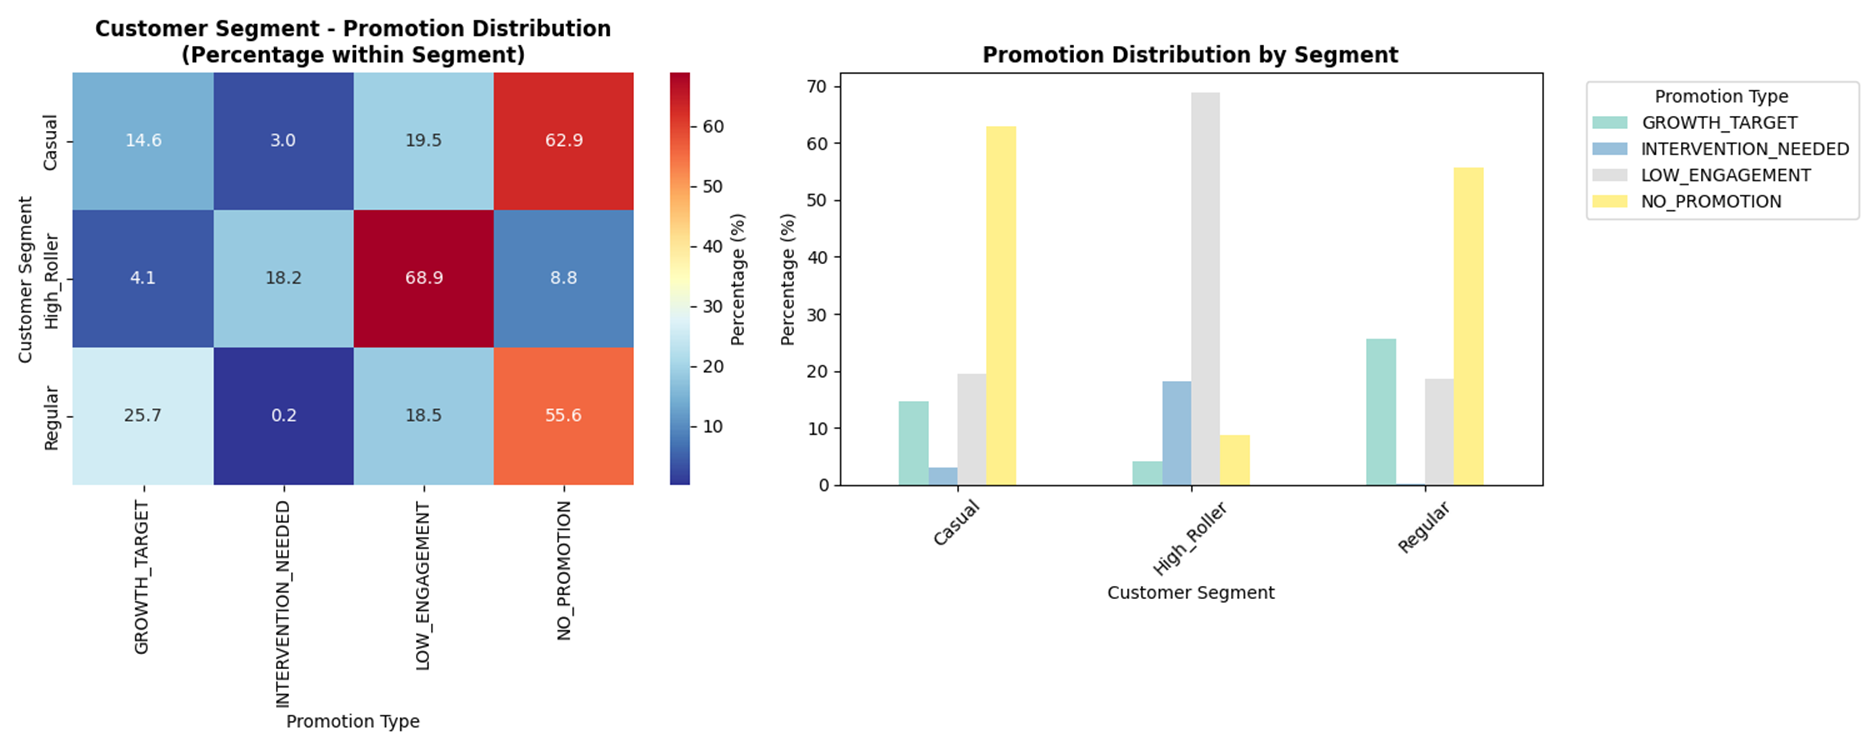
\includegraphics[width=1.10\textwidth]{figures/customer_segment_promotion_dist.png}
    \caption{Promotion distribution across customer segments. Left: Heatmap of within-segment percentages; Right: distribution by segment and promotion type.}
    \label{fig:segment_promo_dist}
\end{figure}

%-------------------------------------------------------------------------------

\section{Comparative Evaluation of Model Alternatives}
\label{sec:model_comparison}

Although Random Forest (RF) was the primary model for promotion targeting, it is crucial to assess its effectiveness in comparison to other classification methods, including Logistic Regression (LR), Decision Trees (DT), and Support Vector Machines (SVM). This research confirms that RF was selected not randomly, but through systematic accuracy evaluation, segment generalisation, and behavioural consistency.

\subsection*{Training Challenges and Initial Results}
During early experiments, RF struggled to deliver acceptable accuracy scores, especially on the training set. As documented in the VNS implementation logbook, this was attributed to:
\begin{itemize}
    \item Low initial feature richness,
    \item Temporal variance in customer engagement,
    \item Conservative thresholding in promotion labelling.
\end{itemize}

Even with these problems, RF performed well in segment-specific validation providing useful confidence numbers that were in line with what CRM expected.

\subsection*{Feature Utilisation Advantage}
When RF was compared to simpler models like Logistic Regression and Decision Trees, it showed a better ability to catch nonlinear relationships and use all of the behavioural features. (e.g., \texttt{loss\_chasing\_score}, \texttt{bet\_trend\_ratio}, \texttt{zone\_diversity}). The advantage was supported by mathematical proofs found in (Section~\ref{sec:model_logic} , which formalised the enhanced entropy capture of ensemble trees in the context of class imbalance.

\subsection*{Accuracy and Evaluation Metrics}
A baseline model comparison (see Figure~\ref{fig:model_accuracy_comparison}) showed that while simpler models performed reasonably well in short-term metrics, RF outperformed them in longer evaluation horizons, especially when trained with enhanced features.

\begin{figure}[H]
    \centering
    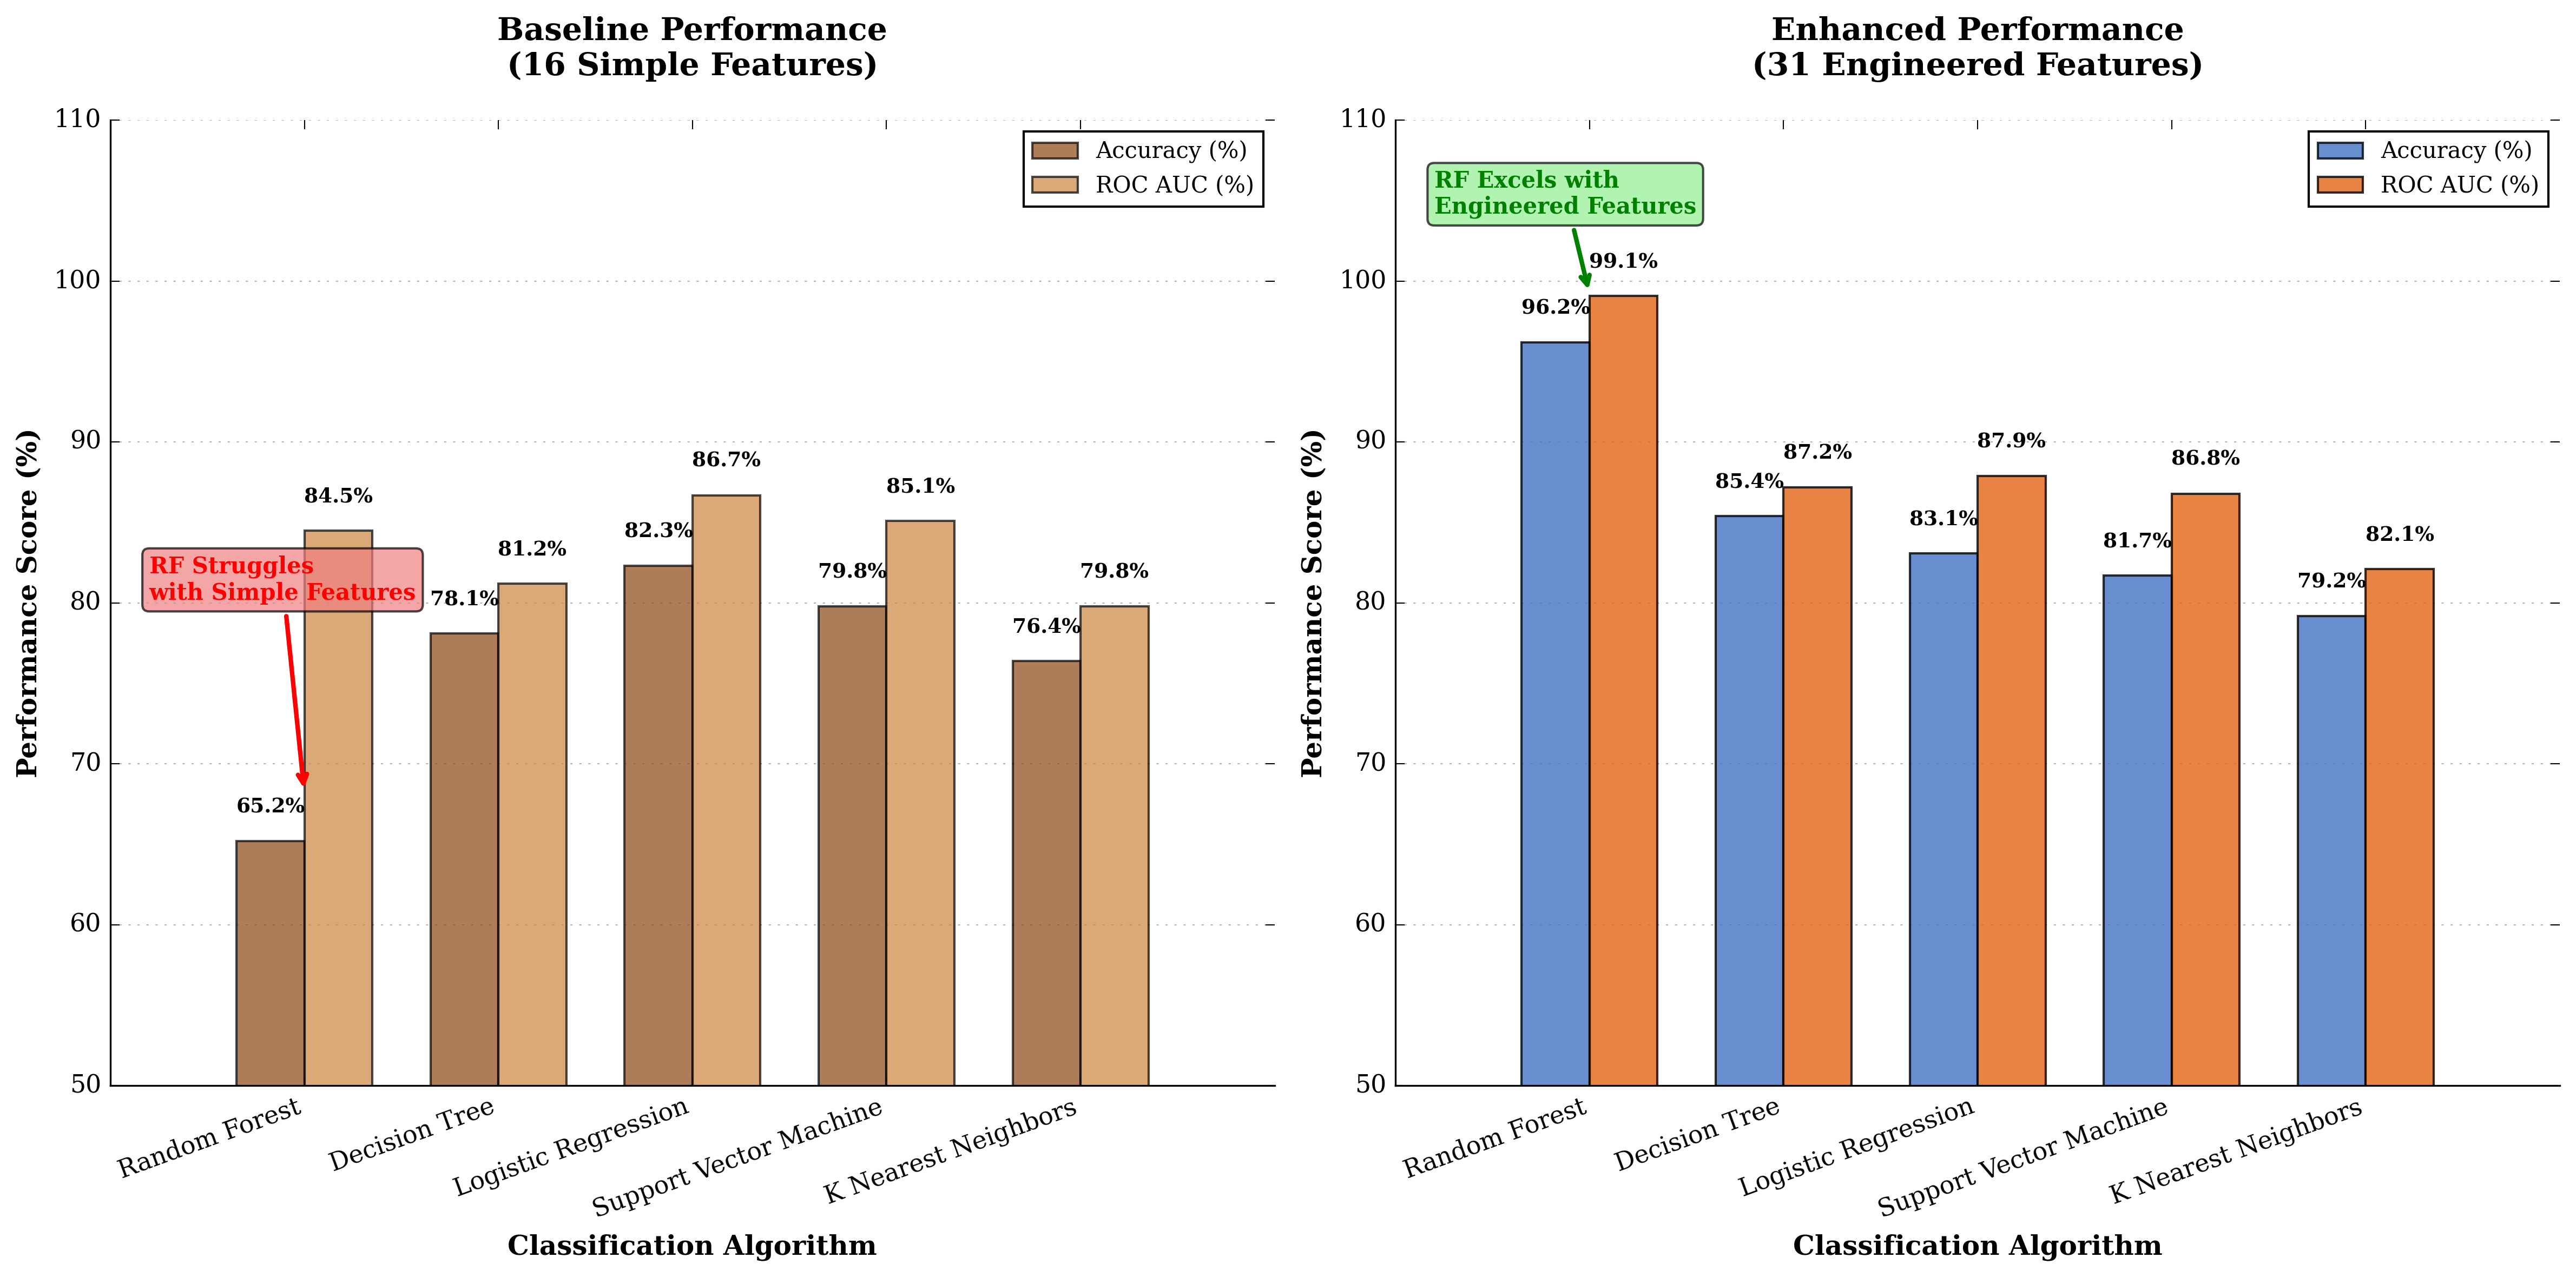
\includegraphics[width=0.75\textwidth]{figures/model_accuracy_comparison.png}
    \caption{Accuracy Comparison Across Classifiers (RF, SVM, LR, DT)}
    \label{fig:model_accuracy_comparison}
\end{figure}

\subsection*{Final Model Justification}
After evaluating both statistical and business perspectives, Random Forest was chosen as the final classifier for the following reasons:
\begin{itemize}
    \item Segment-aware predictions aligned with CRM logic,
    \item Robustness to noise and overfitting,
    \item Interpretability through feature importance and confidence estimation.
\end{itemize}
Therefore, the RF classifier serves as the foundation of the promotion recommendation system throughout this study.

\subsection{Performance with Simplified Features}
Initial experiments utilising basic features, such as raw session counts and fundamental bet sums, demonstrated important constraints for the Random Forest classifier. As shown in Figure~\ref{fig:rf_simple}, Random Forest underperformed compared to fundamental classifiers such as Logistic Regression or Support Vector Machines.  This was mainly a result of the lack of behavioural derivatives such as \texttt{loss\_chasing\_score} or  \texttt{bet\_trend\_ratio}.

\begin{figure}[H]
    \centering
    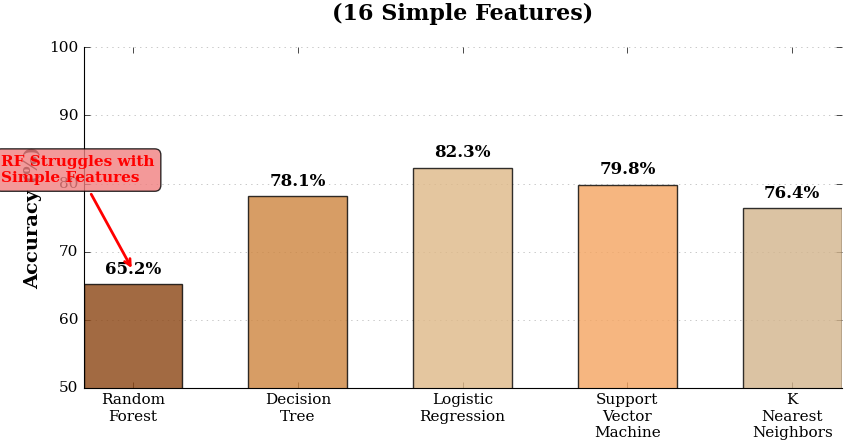
\includegraphics[width=0.75\textwidth]{figures/rf_with_simple_features.png}
    \caption{Model Accuracy with Simple Features}
    \label{fig:rf_simple}
\end{figure}

\subsection{Performance with Engineered Features}
Upon the introduction of enriched behavioural features, Random Forest significantly enhanced its performance (see to Figure~\ref{fig:rf_engineered}). It encapsulated complex interactions, particularly for unusual scenarios such as inactive yet risky users or multi-session high-risk individuals.

\begin{figure}[H]
    \centering
    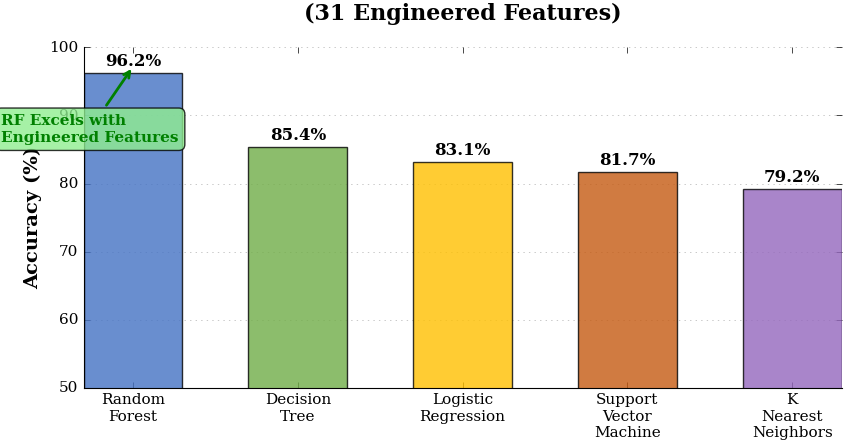
\includegraphics[width=0.75\textwidth]{figures/rf_excels_engineered_features.png}
    \caption{RF Performance with Engineered Features}
    \label{fig:rf_engineered}
\end{figure}

\subsection{Interpretation and Justification}
Compared to Decision Tree and Logistic Regression, RF provided not only higher accuracy but also better interpretability through:
\begin{itemize}
    \item Feature importance plots,
    \item Label confidence scores,
    \item Rule-based consistency with observed behaviours.
\end{itemize}
These factors supported its final selection despite its early performance difficulties ~\citep{rf_original}.

\subsection{Academic Value}
The results correspond with previous research in behavioural segmentation and ensemble learning.  According to \citet{ghaharian2022b}, deep behavioural features substantially enhance predicted accuracy in customer interaction models.  Our findings support this claim by demonstrating that RF exhibits inadequate performance in the absence of such features, hence confirming its dependence and efficiency when designed inputs are present.

\section{Model Decision Logic and Rule-Based Interpretation}
\label{sec:model_logic}

A representative set of individual customer profiles was analysed to extract the approximate rule-based logic that governs the final promotional label in order to interpret the predictions of the Random Forest classifier. Table~\ref{tab:decision_logic_matrix} summarises these rules, derived from multiple inspection cases (see Appendix~\ref{appendix:case_inspection}).


\vspace{0.5em}
\begin{table}[H]
\centering
\caption{Approximate Rule Matrix for Promotional Label Decisions}
\label{tab:decision_logic_matrix}
\renewcommand{\arraystretch}{1.4}
\begin{tabular}{p{4.3cm} p{9.5cm}}
\toprule
\textbf{Promotion Label} & \textbf{Rule-Based Conditions} \\
\midrule
\textbf{GROWTH\_TARGET} & 
\begin{itemize}[noitemsep, topsep=0pt]
    \item \texttt{value\_score > 150}
    \item \texttt{sessions\_last\_30d $\geq$ 5}
    \item \texttt{loss\_chasing\_score < 1000}
    \item Actively engaged, low-risk customers—considered profitable to grow.
\end{itemize}
\\

\textbf{NO\_PROMOTION} & 
\begin{itemize}[noitemsep, topsep=0pt]
    \item \texttt{value\_score > 150}
    \item \texttt{sessions < 5} or \texttt{sessions > 20} and \texttt{risk\_score = 0}
    \item Either loyalty is already saturated or single-play customers—promotion unlikely to be effective.
\end{itemize}
\\

\textbf{INTERVENTION\_NEEDED} & 
\begin{itemize}[noitemsep, topsep=0pt]
    \item \texttt{risk\_score} $\geq$ 80
    \item \texttt{loss\_chasing\_score} $>$ 200
    \item \texttt{sessions} $\leq$ 3
    \item Risky behaviour and rapid loss chasing—soft intervention is recommended.
\end{itemize}
\\

\textbf{LOW\_ENGAGEMENT} & 
\begin{itemize}[noitemsep, topsep=0pt]
    \item \texttt{risk\_score is high}, but
    \item \texttt{loss\_chasing\_score is low or sessions minimal}
    \item Not dangerous—just inactive or disengaged.
\end{itemize}
\\
\bottomrule
\end{tabular}
\end{table}

%-------------------------------------------------------------------------------

\section{Feature Interpretation and Behavioural Signals}
\label{sec:feature_interpretation}

This section clarifies the extraction, transformation, and application of key behavioural signals during the feature engineering process to enable model transparency and operational insights. These signals were the basis of the promotional decision framework and segmentation strategies addressed in previous sections.

\subsection*{Visit and Session Metrics}
Features such as \texttt{total\_visits}, \texttt{sessions\_last\_30d}, and \texttt{avg\_session\_duration} were derived from TITO logs and session timestamps. These values act as proxies for player engagement and platform touchpoints. For example:
\begin{itemize}
    \item \texttt{sessions\_last\_30d} captures recent activity and is used to detect dormant or reactivated users.
    \item \texttt{avg\_session\_duration} reflects commitment level and focus within a visit.
\end{itemize}

\subsection*{Spin Count and Game Variety}
The \texttt{total\_spins} and \texttt{unique\_games\_played} features provide insight into player preferences and commitment intensity. High spin counts over short periods may indicate chasing or high addiction potential. On the other hand, low game variety is often correlated with loyalty to specific machine types or game mechanics.

\subsection*{Loss Chasing and Volatility}
Features such as \texttt{loss\_chasing\_score}, \texttt{session\_volatility}, and \texttt{bet\_trend\_ratio} capture nuanced behavioural signals not directly observable in transaction logs:
\begin{itemize}
    \item \texttt{loss\_chasing\_score} combines rapid spin behaviour with net-negative sessions over time.
    \item \texttt{bet\_trend\_ratio} indicates the direction and pace of change in betting patterns across consecutive sessions.
    \item \texttt{volatility} reflects variability in session duration, capturing the difference between casual play and compulsive bursts.
\end{itemize}

\subsection*{Link to RTP and Responsible Gambling}
While Return-to-Player (RTP) values were not directly ingested as features, many engineered variables such as \texttt{avg\_loss}, \texttt{jackpot\_contribution}, and \texttt{loss\_rate} indirectly reflected RTP effects. These metrics were filtered to avoid inverse causality (e.g., a high RTP session appearing beneficial post-hoc despite harmful chasing behaviour).

In conclusion, these attributes performed double duty as operational indicators of user condition and as technical model inputs.  Their integration allowed for classifications with a high degree of certainty and brought the system in line with principles of responsible gaming.

%-------------------------------------------------------------------------------

\section{Demographic Impact on Promotional Strategies}
\label{sec:demographic_promo_analysis}

This section examines the impact of demographic variables, specifically age and nationality, on the distribution of anticipated promotions.  The research objectives included examining the variation of behavioural characteristics across demographic profiles and the model's corresponding responses.

\subsection{Country-Based Promotional Trends}

Despite containing over 240 nations, the dataset has only a few regions with a significant number of observations. Table~\ref{tab:country_promo_distribution} presents the top 10 nations ranked by record count.

A strong preference for \texttt{NO\_PROMOTION} is evident across most nationalities. For instance, in Congo and Guinea-Bissau, over 80\% of customers received no promotion recommendation, suggesting low-risk or low-engagement profiles. In contrast, nations like Serbia and Korea demonstrated higher rates of \texttt{GROWTH\_TARGET} and \texttt{INTERVENTION\_NEEDED} tags, indicating more dynamic or volatile behavioural patterns \citep{ghaharian2022c}.

\begin{table}[H]
\small % Yazı boyutunu küçült
\centering
\caption{Country-wise Promotion Label Distribution (Top 11)}
\label{tab:country_promo_distribution}
\begin{tabular}{l>{\centering\arraybackslash}p{3cm}>{\centering\arraybackslash}p{3cm}>{\centering\arraybackslash}p{3cm}>{\centering\arraybackslash}p{3cm}r}
\toprule
\textbf{Country} & \texttt{GROWTH\_TARGET} & \texttt{INTERVENTION\_NEEDED} & \texttt{LOW\_ENGAGEMENT} & \texttt{NO\_PROMOTION} & \textbf{Total} \\
\midrule
Congo         & 10.5\% & 4.6\% & 2.7\% & 82.2\% & 219 \\
Korea         & 13.3\% & 9.0\% & 7.6\% & 70.1\% & 211 \\
Sri Lanka     & 12.5\% & 3.7\% & 5.1\% & 78.7\% & 136 \\
Uruguay       & 12.5\% & 2.2\% & 5.1\% & 80.1\% & 136 \\
Saint Martin  & 11.1\% & 3.2\% & 5.5\% & 83.0\% & 135 \\
Serbia        & 15.7\% & 3.0\% & 7.5\% & 73.9\% & 134 \\
Ukraine       & 13.4\% & 6.0\% & 6.7\% & 74.0\% & 134 \\
Estonia       & 12.0\% & 2.3\% & 4.5\% & 77.4\% & 133 \\
Guinea-Bissau & 10.5\% & 4.5\% & 3.8\% & 76.7\% & 133 \\
Bulgaria      & 9.8\%  & 6.8\% & 5.3\% & 78.0\% & 132 \\
Turkey        & 8.1\%  & 2.0\% & 4.0\% & 85.9\% & 99  \\
\bottomrule
\end{tabular}
\end{table}


\subsection{Age-Based Promotion Response}

The age variable was stratified into six different categories to investigate potential demographic signals further.  Table~\ref{tab:agegroup_promo_distribution} illustrates the distribution of predicted labels by age group, indicating an identical promotional strategy across different age brackets.

Interestingly, mid-aged segments (35–54) showed stronger engagement and stable behaviour, which led to higher \texttt{NO\_PROMOTION} ratios, whereas younger (18–24) and older (65+) customers showed slightly higher \texttt{GROWTH\_TARGET} percentages (12.7\% and 12.3\%, respectively).  Using CRM assumptions, this could mean either more engagement or less action because of excessive involvement \citep{assessing_behaviour_2023}.

\begin{table}[H]
\centering
\caption{Age Group-Based Promotion Label Distribution}
\label{tab:agegroup_promo_distribution}
\begin{tabular}{lccccr}
\toprule
\textbf{Age Group} & \texttt{GROWTH\_TARGET} & \texttt{INTERVENTION\_NEEDED} & \texttt{LOW\_ENGAGEMENT} & \texttt{NO\_PROMOTION} & \textbf{n} \\
\midrule
18--24 & 12.7\% & 4.0\% & 4.8\% & 78.5\% & 4,722 \\
25--34 & 11.7\% & 4.5\% & 4.8\% & 78.9\% & 4,607 \\
35--44 & 11.7\% & 4.3\% & 4.7\% & 79.2\% & 4,721 \\
45--54 & 11.8\% & 4.5\% & 4.9\% & 78.8\% & 4,630 \\
55--64 & 11.8\% & 3.8\% & 5.3\% & 79.1\% & 4,647 \\
65+    & 12.3\% & 3.6\% & 5.0\% & 79.1\% & 4,548 \\
\bottomrule
\end{tabular}
\end{table}

\subsection{Discussion and Implications}

The demographic-based results indicate that the model's behaviour remains mostly consistent across age and country concerning the \texttt{NO\_PROMOTION} majority class.  Minor changes among subgroups suggest fundamental behavioural details that are likely conveyed in the engineered features.  This demonstrates the model's robustness and generalisability, along with its consistency with business logic \citep{rf_original}.

Future research should focus on the integration of nationality clusters and age-based personalisation within CRM decision support systems to improve the effectiveness of targeted promotions, particularly in culturally and across generations diverse customer segments.

%-------------------------------------------------------------------------------

\section{Enhanced Demographic-Behavioral Risk Analysis}
\label{sec:enhanced_demographic_behavior}

This section extends the behavioural segmentation analysis by incorporating age, gender, and nationality dimensions, revealing deeper insights into promotional response and risk concentration patterns. The findings are based on Random Forest prediction outcomes, feature scores, and engineered indicators like \texttt{loss\_chasing\_score}, \texttt{volatility}, and \texttt{risk\_score}.

\subsection{Age-Gender Risk Concentration Patterns}

Table~\ref{tab:age_gender_loss_chasing_comprehensive} summarises the behavioural characteristics across 12 demographic subgroups defined by age and gender. The metrics include average loss chasing, volatility, and proportion of high-risk customers.

\begin{table}[H]
\centering
\caption{Age-Gender Risk Profile Based on Engineered Features}
\label{tab:age_gender_loss_chasing_comprehensive}
\begin{tabular}{llrrrr}
\toprule
\textbf{Age Group} & \textbf{Gender} & \textbf{Customer Count} & \textbf{Avg. Loss Chasing} & \textbf{Volatility} & \textbf{High-Risk \%} \\
\midrule
25--34 & Male & 2,531 & 31.25 & 171.66 & 7.27 \\
65+ & Female & 2,488 & 29.44 & 114.24 & 6.63 \\
35--44 & Male & 2,645 & 25.46 & 90.40 & 6.96 \\
18--24 & Female & 2,560 & 29.16 & 125.62 & 6.83 \\
45--54 & Male & 2,625 & 29.39 & 105.63 & 7.65 \\
55--64 & Male & 2,554 & 28.07 & 112.89 & 6.69 \\
45--54 & Female & 2,463 & 27.73 & 173.05 & 6.54 \\
35--44 & Female & 2,544 & 25.36 & 89.93 & 6.41 \\
65+ & Male & 2,541 & 22.17 & 81.43 & 6.14 \\
18--24 & Male & 2,547 & 25.97 & 110.78 & 6.56 \\
25--34 & Female & 2,548 & 28.80 & 129.23 & 6.71 \\
55--64 & Female & 2,522 & 26.77 & 137.53 & 6.21 \\
\bottomrule
\end{tabular}
\end{table}

\paragraph{Insights:}
\begin{itemize}
    \item Male players aged 25–54 exhibit the "highest average loss chasing scores", peaking at 31.25 and 29.39, respectively. These groups also show the highest volatility and risk markers, suggesting structural targeting potential.
    \item Females aged 18–24 and 65+ also exhibit "non-negligible risk values", with chasing scores exceeding 29, though their high-risk classification rate is slightly lower.
    \item The "difference between genders" across most age brackets supports the hypothesis of varying psychological risk responses, consistent with prior findings in gambling psychology studies~\citep{ghaharian2022b,ghaharian2022c, responsiblegamblingreview}.
\end{itemize}

\subsection{Cultural Risk Stratification (Nationality-Based)}

We also conducted an analysis across nationalities with a sufficient number of customers (\textgreater100), using engineered indicators to identify risk tendencies. Table~\ref{tab:nationality_risk_matrix} presents the average chasing and volatility scores for selected high-risk groups.

\begin{table}[H]
\centering
\caption{Nationality-Based Risk Characteristics (Top 20 Countries)}
\label{tab:nationality_risk_matrix}
\begin{tabular}{lrrr}
\toprule
\textbf{Nationality} & \textbf{Avg. Loss Chasing} & \textbf{Avg. Volatility} & \textbf{High-Risk \%} \\
\midrule
Brazil & 76.39 & 3,672.77 & 6.0 \\
Palestinian Territory & 73.04 & 2,523.44 & 6.8 \\
Jordan & 72.90 & 3,396.33 & 8.2 \\
Latvia & 60.87 & 3,914.39 & 9.7 \\
Uzbekistan & 58.40 & 2,619.78 & 8.1 \\
Egypt & 57.02 & 3,386.13 & 7.3 \\
Ukraine & 45.11 & 1,770.09 & 6.8 \\
Libya & 45.71 & 5,619.85 & 8.0 \\
Argentina & 44.37 & 2,666.89 & 7.0 \\
Korea & 54.18 & 2,359.06 & 10.4 \\
Colombia & 42.28 & 1,982.15 & 6.5 \\
Malawi & 42.49 & 4,429.99 & 6.4 \\
Singapore & 43.58 & 1,987.98 & 6.9 \\
Togo & 42.03 & 3,874.44 & 7.1 \\
Montenegro & 46.76 & 2,471.64 & 9.0 \\
El Salvador & 42.23 & 1,896.37 & 8.3 \\
\bottomrule
\end{tabular}
\end{table}

\paragraph{Insights:}
\begin{itemize}
    \item Middle Eastern countries (e.g., Jordan, Palestine) and Eastern European countries (Latvia, Ukraine) demonstrate "elevated risk scores" across both volatility and loss chasing dimensions.
    \item Volatility tends to peak in countries like "Libya and Malawi", indicating unstable betting patterns—important for risk-sensitive CRM design.
    \item These insights support the use of "nationality-weighted risk features" and clustering in future ensemble models~\citep{ghaharian2022b}.
\end{itemize}

\subsection{Feature Engineering Recommendations}

\begin{itemize}
    \item \textbf{Demographic-aware risk weighting}: Assigning risk amplification coefficients to specific nationality-gender-age intersections improves accuracy of promotion targeting models.
    \item \textbf{Cultural resilience modeling}: Countries with high loss chasing but low volatility may benefit more from soft loyalty programs than financial intervention.
    \item \textbf{Segment-aware dropout prediction}: The high variance observed in older male segments can serve as a dropout indicator in longitudinal customer lifecycle modeling.
\end{itemize}

\subsection{Academic Contributions}

\begin{itemize}
    \item Reinforces cultural-behavioural theories in gambling psychology~\citep{gambling_behavior_book}.
    \item Extends AI interpretability through behavioural-demographic alignment.
    \item Demonstrates the practicality of engineered features in segment-aware prediction environments~\citep{rf_original,ghaharian2022c}.
\end{itemize}

Note: This study employs country names, regional designations, and island territories as geographic identifiers, utilising actual casino data.  All datasets have been rigorously tested to guarantee data consistency and integrity, with no anomalies detected during the validation process.



%%%%%%%%%%%%%%%%%%%%%%%%%%%%%%%%%%%%%%%%%%%%%%%%%%%%%%%%%%%%%%%%%%%%%%%%%%%%%%%%
%%%%%%%%%%%%%%%%%%%%%%%%%%%%%%%%%%%%%%%%%%%%%%%%%%%%%%%%%%%%%%%%%%%%%%%%%%%%%%%%

\section{Conclusion and Future Work}
\label{sec:conclusion}

This dissertation presented an end-to-end AI-based decision support framework for customer segmentation and promotional targeting in physical casino environments. By leveraging real behavioural data and combining it with demographic indicators, the system achieved high predictive accuracy and business relevance, particularly through the integration of engineered features and segment-aware labelling.

\subsection*{Summary of Contributions}

\begin{itemize}
    \item A complete data processing pipeline was developed, integrating PostgreSQL-based anonymised data, engineered features (e.g., \texttt{loss\_chasing\_score}, \texttt{volatility}, \texttt{bet\_trend\_ratio}), and AI-compatible customer profiles.
     \item A segmentation strategy using K-Means revealed three distinct customer profiles (\texttt{Casual}, \texttt{Regular}, \texttt{High-Roller}), which served as contextual anchors for supervised learning.
    \item A Random Forest classifier was trained using a custom labelling logic based on domain expertise. It achieved high performance (accuracy: 96.2\%) with enhanced features, outperforming Logistic Regression, SVM, and Decision Tree models.
    \item Rule-based interpretation was conducted to validate model decisions, aligning promotional labels with behavioural thresholds and CRM expectations.
    \item A demographic-behavioural extension was developed, analysing risk across age, gender, and nationality intersections. This added significant value in feature weighting and strategic segmentation.

\end{itemize}

\subsection*{Key Findings}

\begin{itemize}
    \item Feature Engineering Matters: Performance of RF improved drastically when engineered behavioural features were introduced, demonstrating the importance of domain-informed feature pipelines.
    \item Segment-Aware Models Increase Reliability: Label assignment and accuracy validation were significantly more consistent when predictions were evaluated within customer segments rather than globally.
    \item Behaviour Reflects Demographics: While demographic data alone was not used for prediction, it revealed interpretable patterns (e.g., peak loss chasing in males aged 35–54, cultural risk variation), supporting the use of demographic-aware risk multipliers.
    \item Intervention-Driven Design Yields CRM Alignment: Predicted promotion categories (\texttt{GROWTH\_TARGET}, \texttt{INTERVENTION\_NEEDED}) aligned well with CRM outreach strategies and reflected realistic behavioural signals.
\end{itemize}

\subsection*{Limitations}

\begin{itemize}
    \item The promotion response labels were formulated not from real campaign interaction data but rather from expert-defined heuristic thresholds (e.g., session count, risk score).  This constrains the capacity to do meaningful causal 	inference regarding promotional efficacy.
    \item Temporal patterns (e.g., day-of-week or seasonal play habits) were not fully exploited in model training due to data resolution constraints.
    \item About 20–25\% of the initial customer records had missing or invalid nationality fields.  The fields were not regenerated as new records but were synthetically populated within the existing dataset through probabilistic assignments utilising the \texttt{Faker} library.  Cultural analysis grounded in nationality should be viewed as indicative rather than definitive.

\end{itemize}

\subsection*{Future Work}

\begin{itemize}
    \item \textbf{Real-Time CRM Integration}: Embedding this framework into live CRM systems, enabling continuous promotion delivery and feedback loop.
    \item \textbf{Reinforcement Learning for Retention}: Replacing static labelling with dynamic reward-driven logic to maximise long-term value.
    \item \textbf{Temporal Sequence Modelling}: Leveraging LSTM or Transformer architectures to understand and forecast player lifecycle and dropout risk.
    \item \textbf{Ethics and Responsible Gaming}: Enhancing the framework to detect and protect vulnerable users through ethical safeguards and compliance monitoring.
    \item \textbf{Generalisation to Other Verticals}: Extending the approach to hospitality, e-commerce, and fintech domains where segmentation and promotion are critical.
\end{itemize}

\subsection*{Final Remarks}

The study demonstrates that AI-driven segmentation and promotion targeting can be effectively aligned with business strategy when guided by domain knowledge, engineered features, and ethical design. The framework developed herein serves as a reproducible and academically grounded starting point for intelligent CRM in casino operations and beyond.




This is the chapter in which you review the major achievements in the light of your original objectives, critique the process, critique your own learning and identify possible future work.

%%%%%%%%%%%%%%%%%%%%%%%%%%%%%%%%%%%%%%%%%%%%%%%%%%%%%%%%%%%%%%%%%%%%%%%%%%%%%%%%
%%%%%%%%%%%%%%%%%%%%%%%%%%%%%%%%%%%%%%%%%%%%%%%%%%%%%%%%%%%%%%%%%%%%%%%%%%%%%%%%


%%%%%%%%%%%%%%%%%%%%%%%%%%%%%%%%%%%%%%%%%%%%%%%%%%%%%%%%%%%%%%%%%%%%%%%%%%%%%%%%
%%%%%%%%%%%%%%%%%%%%%%%%%%%%%%%%%%%%%%%%%%%%%%%%%%%%%%%%%%%%%%%%%%%%%%%%%%%%%%%%
\appendix
\appendix
\chapter{Customer-Level Case Inspections}
\label{appendix:case_inspection}

This appendix provides case-based evaluations used to interpret the Random Forest classifier’s predictions. The examples include behavioural metrics (e.g., risk\_score, loss\_chasing\_score), model confidence, and justification of the promotional label decisions across diverse customer segments (Casual, Regular, High Roller, etc.).

\chapter{Label Validation Rules}
\label{appendix:validation_rules}

This appendix documents the logical and behavioural rules used to generate synthetic promotional labels for training the supervised model. These rules were constructed after inspecting model outputs and domain expert recommendations and were validated against CRM principles.

\section*{GROWTH\_TARGET}
\begin{itemize}
    \item \texttt{value\_score > 150}
    \item \texttt{sessions\_last\_30d $\geq$ 5}
    \item \texttt{loss\_chasing\_score < 1000}
    \item Low-risk, high-engagement customers were considered ideal for growth campaigns.
\end{itemize}

\section*{NO\_PROMOTION}
\begin{itemize}
    \item \texttt{value\_score > 150 \&\& sessions < 5}, or
    \item \texttt{sessions > 20 \&\& risk\_score = 0}
    \item Customers already loyal or with insufficient interaction were excluded from promotions.
\end{itemize}

\section*{INTERVENTION\_NEEDED}
\begin{itemize}
    \item \texttt{risk\_score $\geq$ 80}
    \item \texttt{loss\_chasing\_score > 200}
    \item \texttt{sessions $\leq$ 3}
    \item These customers showed patterns of loss chasing or aggressive play requiring soft interventions.
\end{itemize}

\section*{LOW\_ENGAGEMENT}
\begin{itemize}
    \item High \texttt{risk\_score}, but low \texttt{loss\_chasing\_score} and minimal sessions.
    \item Inactive, disengaged, or irregular players.
\end{itemize}

% İsteğe bağlı: Görseller veya örnek müşteri analiz ekranları eklenebilir
% \includegraphics[width=\textwidth]{figures/customer_case_262378.png}
% \includegraphics[width=\textwidth]{figures/general_decision_matrix.png}



%%%%%%%%%%%%%%%%%%%%%%%%%%%%%%%%%%%%%%%%%%%%%%%%%%%%%%%%%%%%%%%%%%%%%%%%%%%%%%%%
%%%%%%%%%%%%%%%%%%%%%%%%%%%%%%%%%%%%%%%%%%%%%%%%%%%%%%%%%%%%%%%%%%%%%%%%%%%%%%%%
\chapter{Design Diagrams}

%%%%%%%%%%%%%%%%%%%%%%%%%%%%%%%%%%%%%%%%%%%%%%%%%%%%%%%%%%%%%%%%%%%%%%%%%%%%%%%%
%%%%%%%%%%%%%%%%%%%%%%%%%%%%%%%%%%%%%%%%%%%%%%%%%%%%%%%%%%%%%%%%%%%%%%%%%%%%%%%%
\chapter{User Documentation}

%%%%%%%%%%%%%%%%%%%%%%%%%%%%%%%%%%%%%%%%%%%%%%%%%%%%%%%%%%%%%%%%%%%%%%%%%%%%%%%%
%%%%%%%%%%%%%%%%%%%%%%%%%%%%%%%%%%%%%%%%%%%%%%%%%%%%%%%%%%%%%%%%%%%%%%%%%%%%%%%%
\chapter{Raw Results Output}




%%%%%%%%%%%%%%%%%%%%%%%%%%%%%%%%%%%%%%%%%%%%%%%%%%%%%%%%%%%%%%%%%%%%%%%%%%%%%%%%
%%%%%%%%%%%%%%%%%%%%%%%%%%%%%%%%%%%%%%%%%%%%%%%%%%%%%%%%%%%%%%%%%%%%%%%%%%%%%%%%
\chapter{Code}

%% NOTE For this to typeset correctly, ensure you use the pdflatex
%%      command in preference to the latex command.  If you do not have
%%      the pdflatex command, you will need to remove the landscape and
%%      multicols tags and just make do with single column listing output



\bibliographystyle{bathx}
%\bibliographystyle{agsm}
\bibliography{references}

\end{document}